

\section{Measurement of \texorpdfstring{$j \to \tau_h$}{Lg} Scale Factor}


In both our signal region and control region, $\mu \tau$ and $e \tau$
final states have sizable contributions from electron or muon plus a jet
misidentified as a hadronic tau.  For correction to tau identification
efficiency, tau POG has provided $SF (\tau_h \to \tau_h)$ measured with
tag-prob technique at different identification working points.  However,
regarding $SF (j \to \tau_h)$, because the jet environment varies from
analysis to analysis, tau POG suggests us to measure it ourselves in a
side-band region to correct $j \to \tau_h$ contributions and access
corresponding uncertainties.

Our measurement of $SF (j\to \tau_h)$ is based on two regions,
$t\bar{t}$ region which is enriched with b-jets identified as hadronic
taus, $Z+jets$ region which is enriched with light jets identified as
hadronic taus.

\begin{itemize}
    \item $t\bar{t}$ region: $e\mu+\tau_h$ final state is selected. The selection requires
    exactly one muon and one electron with tight identification and
    isolation, plus one hadronic tau passing VTight working point.
    Corrections to reconstruction and selection of electron and muon are
    applied.
    The events has to fire either single muon trigger or single electron
    trigger.  The pT threshold for triggering muon (electron) is 25 (30)
    GeV, while for non-triggering muon (electron) is 10 (20) GeV.  This
    selects a sample enriched with $t\bar{t}$ where a b jet is
    misidentified as $\tau_h$. The kinematics of $e\mu+tau$ final
    state events are shown in Figure~\ref{fig:appendix:fakeTauId:emutau}.
    
    
    \item $Z+jets$ region: $\mu\mu+\tau_h$ and $ee+\tau_h$ final state are selected.  The
    selection requires exactly two muons or two electrons with tight
    identification and isolation, plus one hadronic tau passing VTight
    working point.  Corrections to reconstruction and selection of
    electron and muon are applied.
    The trigger and pT thresholds of leptons are the same as
    $e\mu+\tau_h$ final state.  This selects a sample enriched with $Z +
    jet$ where a light jet is misidentified as $\tau_h$. The kinematics of $\mu\mu+tau$ and
    $ee+\tau$ final states are shown in Figure~\ref{fig:appendix:fakeTauId:mumutau} and \ref{fig:appendix:fakeTauId:eetau}.
\end{itemize}


\begin{figure}
    \centering
    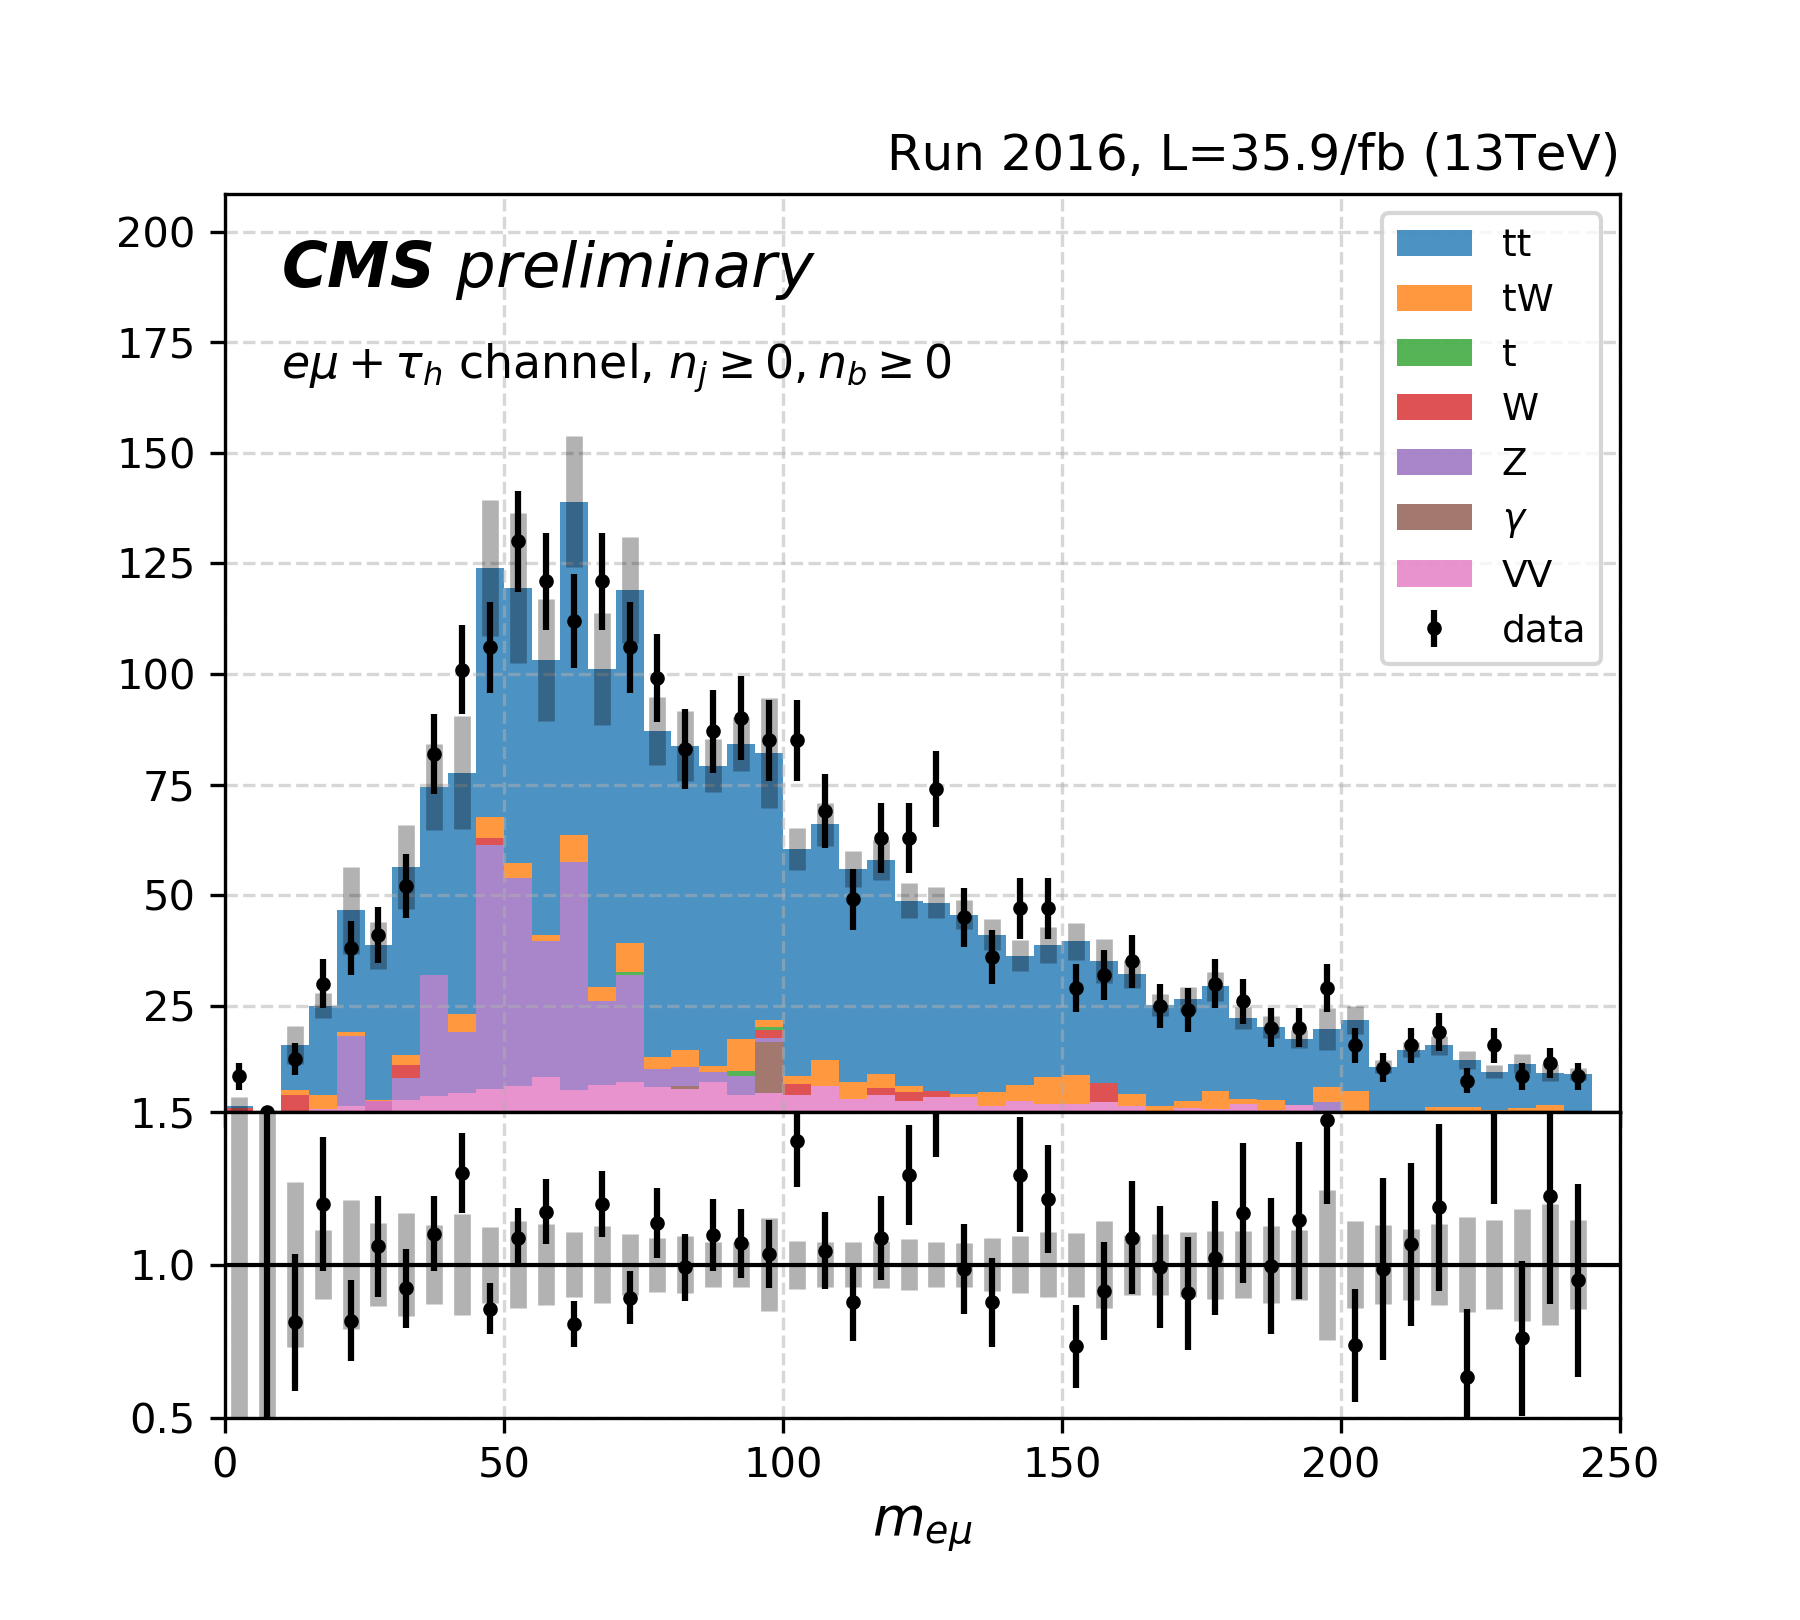
\includegraphics[width=0.4\textwidth]{chapters/Appendix/sectionJetToTauh/figures/emutau_dilepton_mass_pickles_lltauTight.png}
    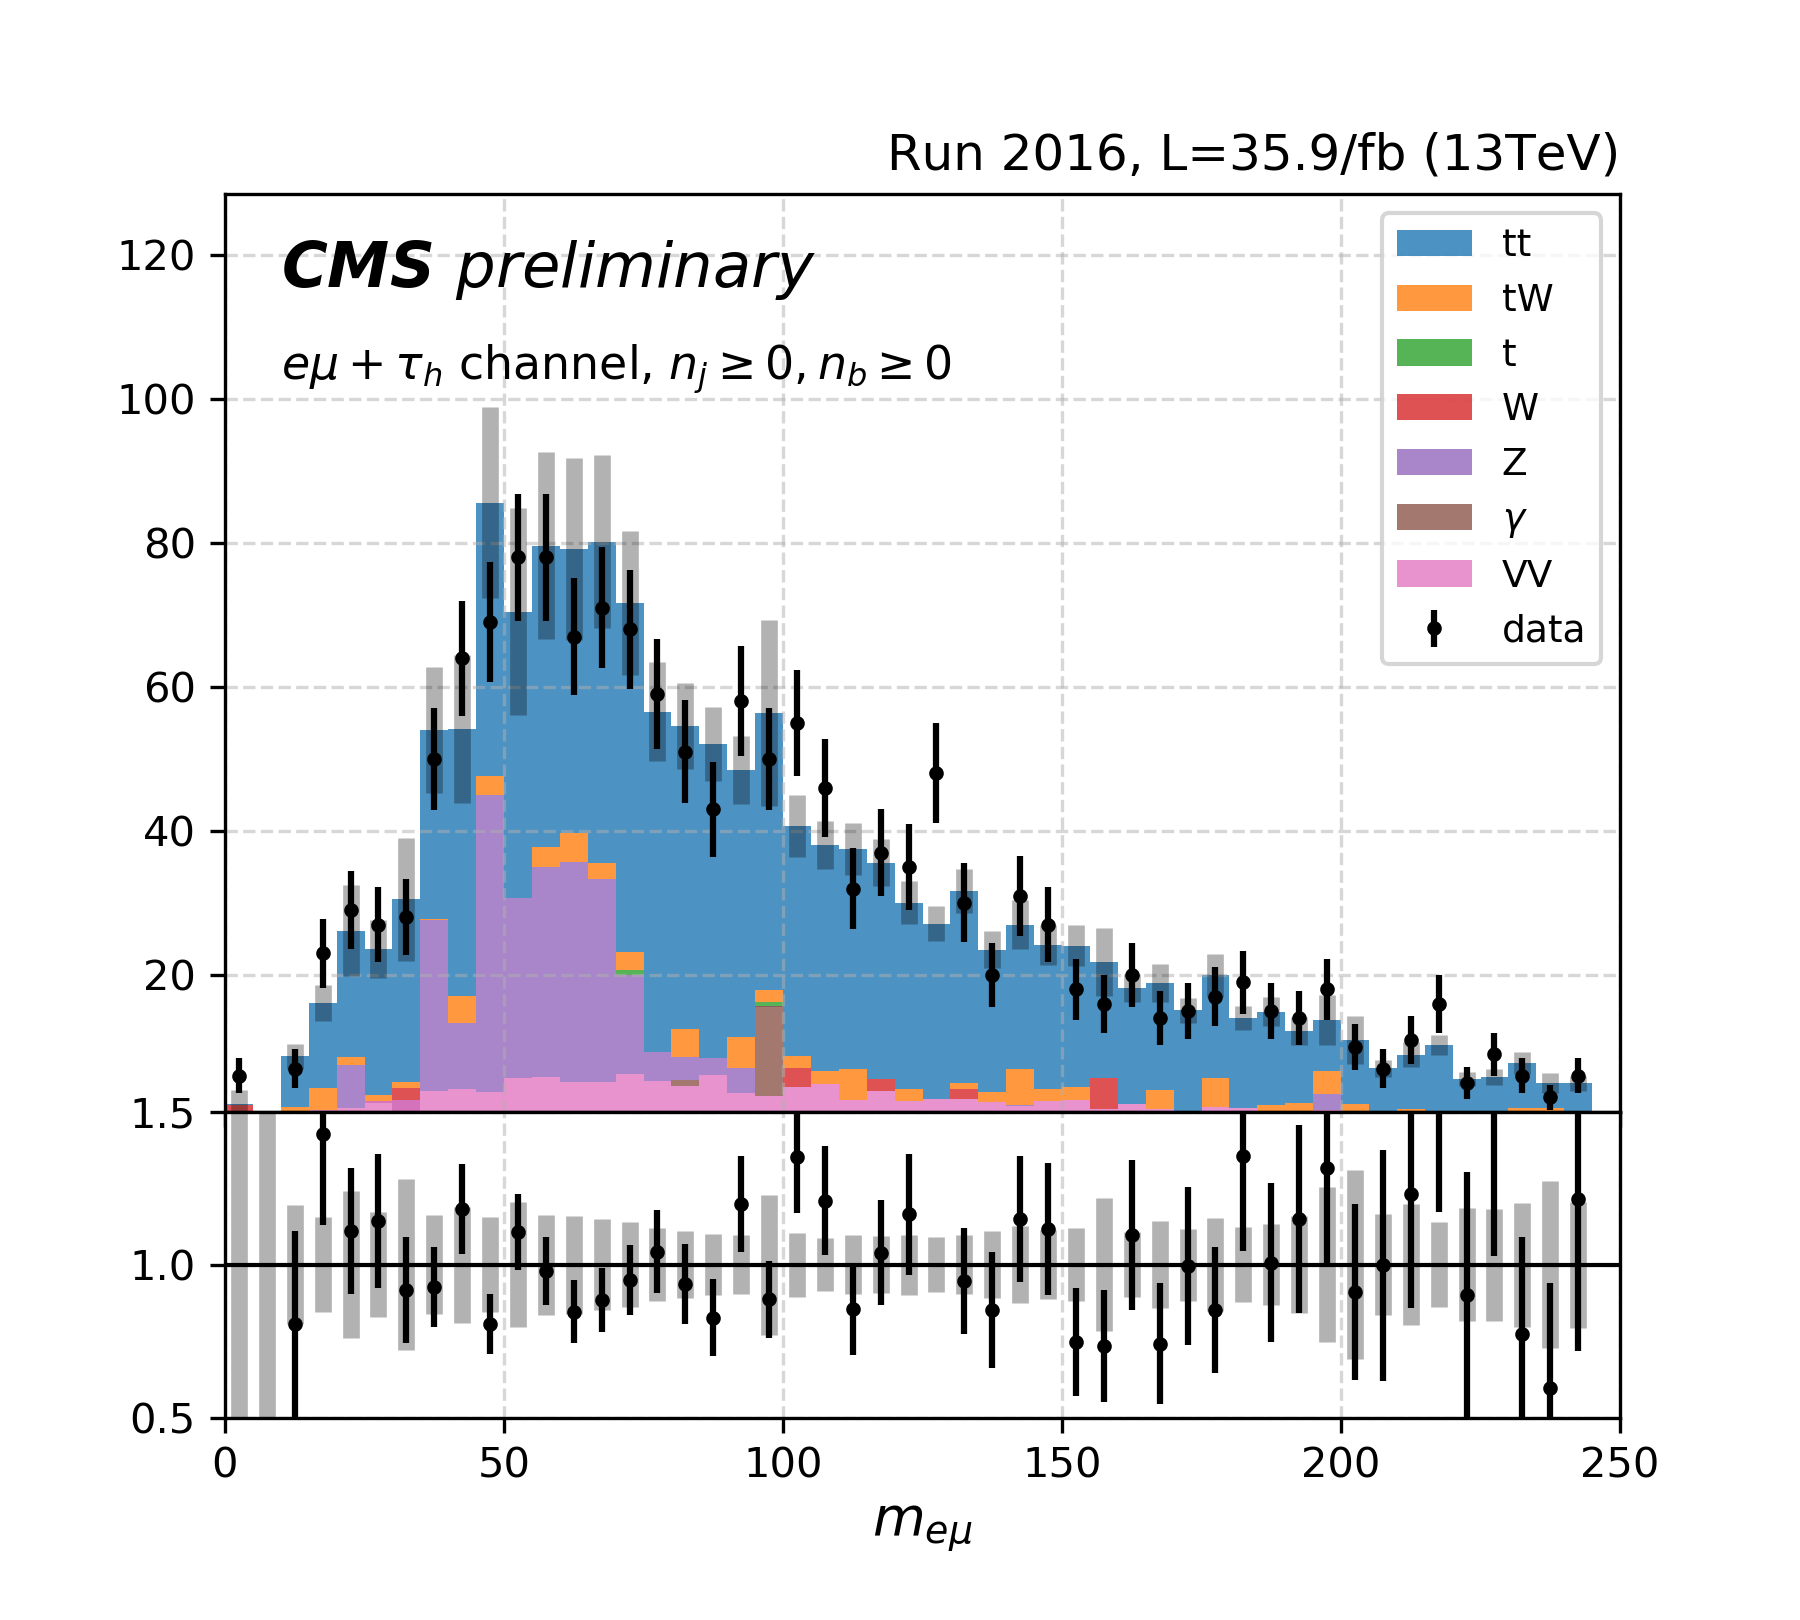
\includegraphics[width=0.4\textwidth]{chapters/Appendix/sectionJetToTauh/figures/emutau_dilepton_mass_pickles_lltauVTight.png}
    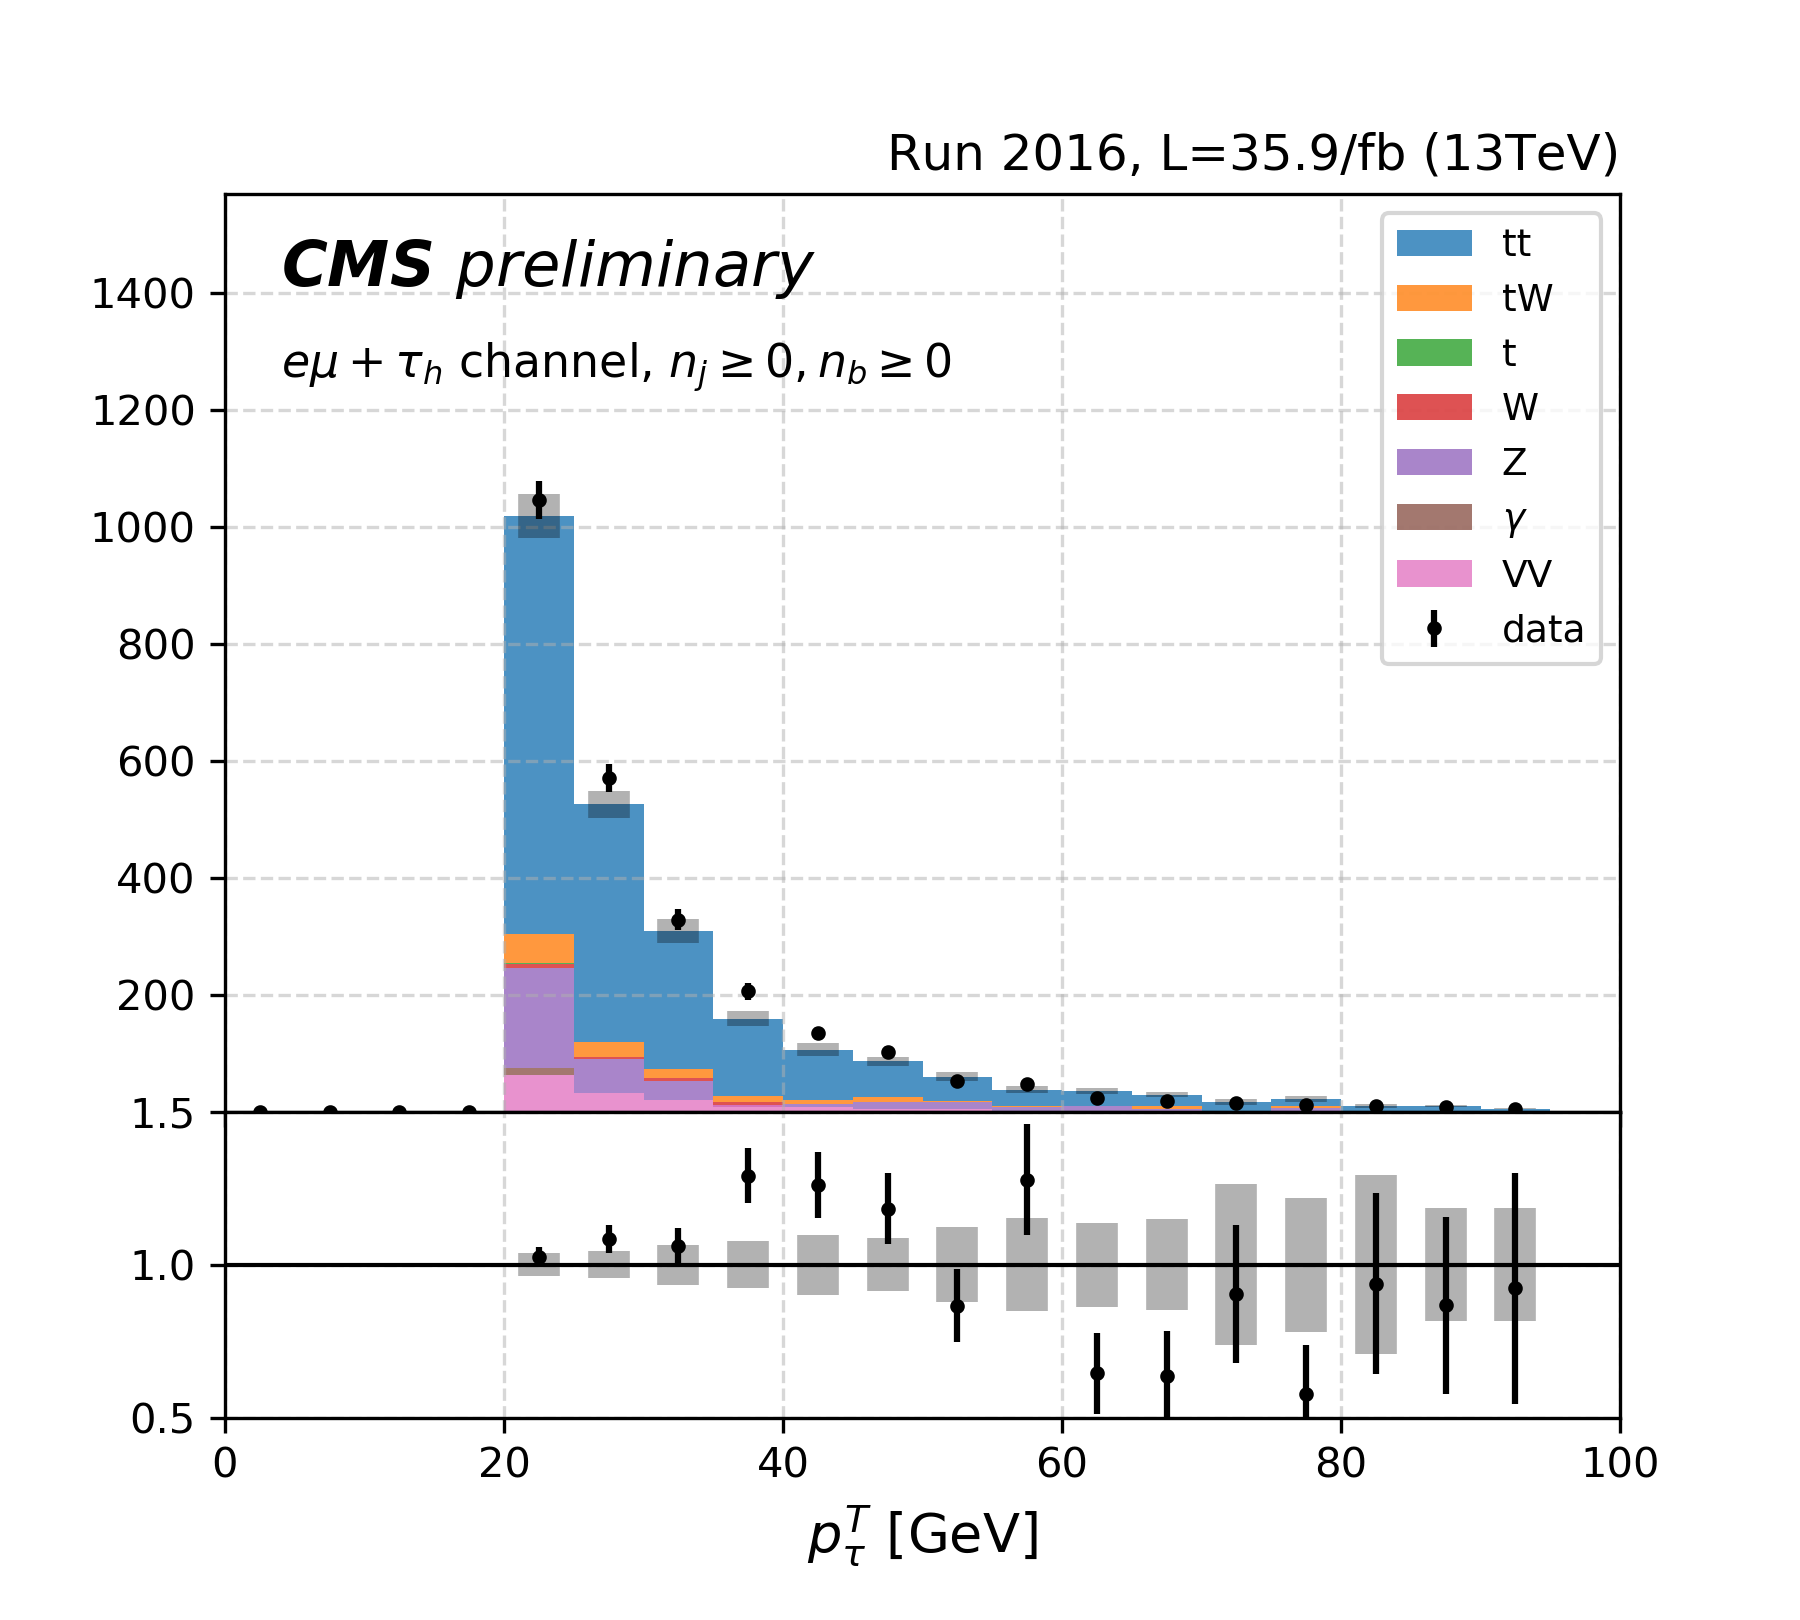
\includegraphics[width=0.4\textwidth]{chapters/Appendix/sectionJetToTauh/figures/emutau_tauPt_pickles_lltauTight.png}
    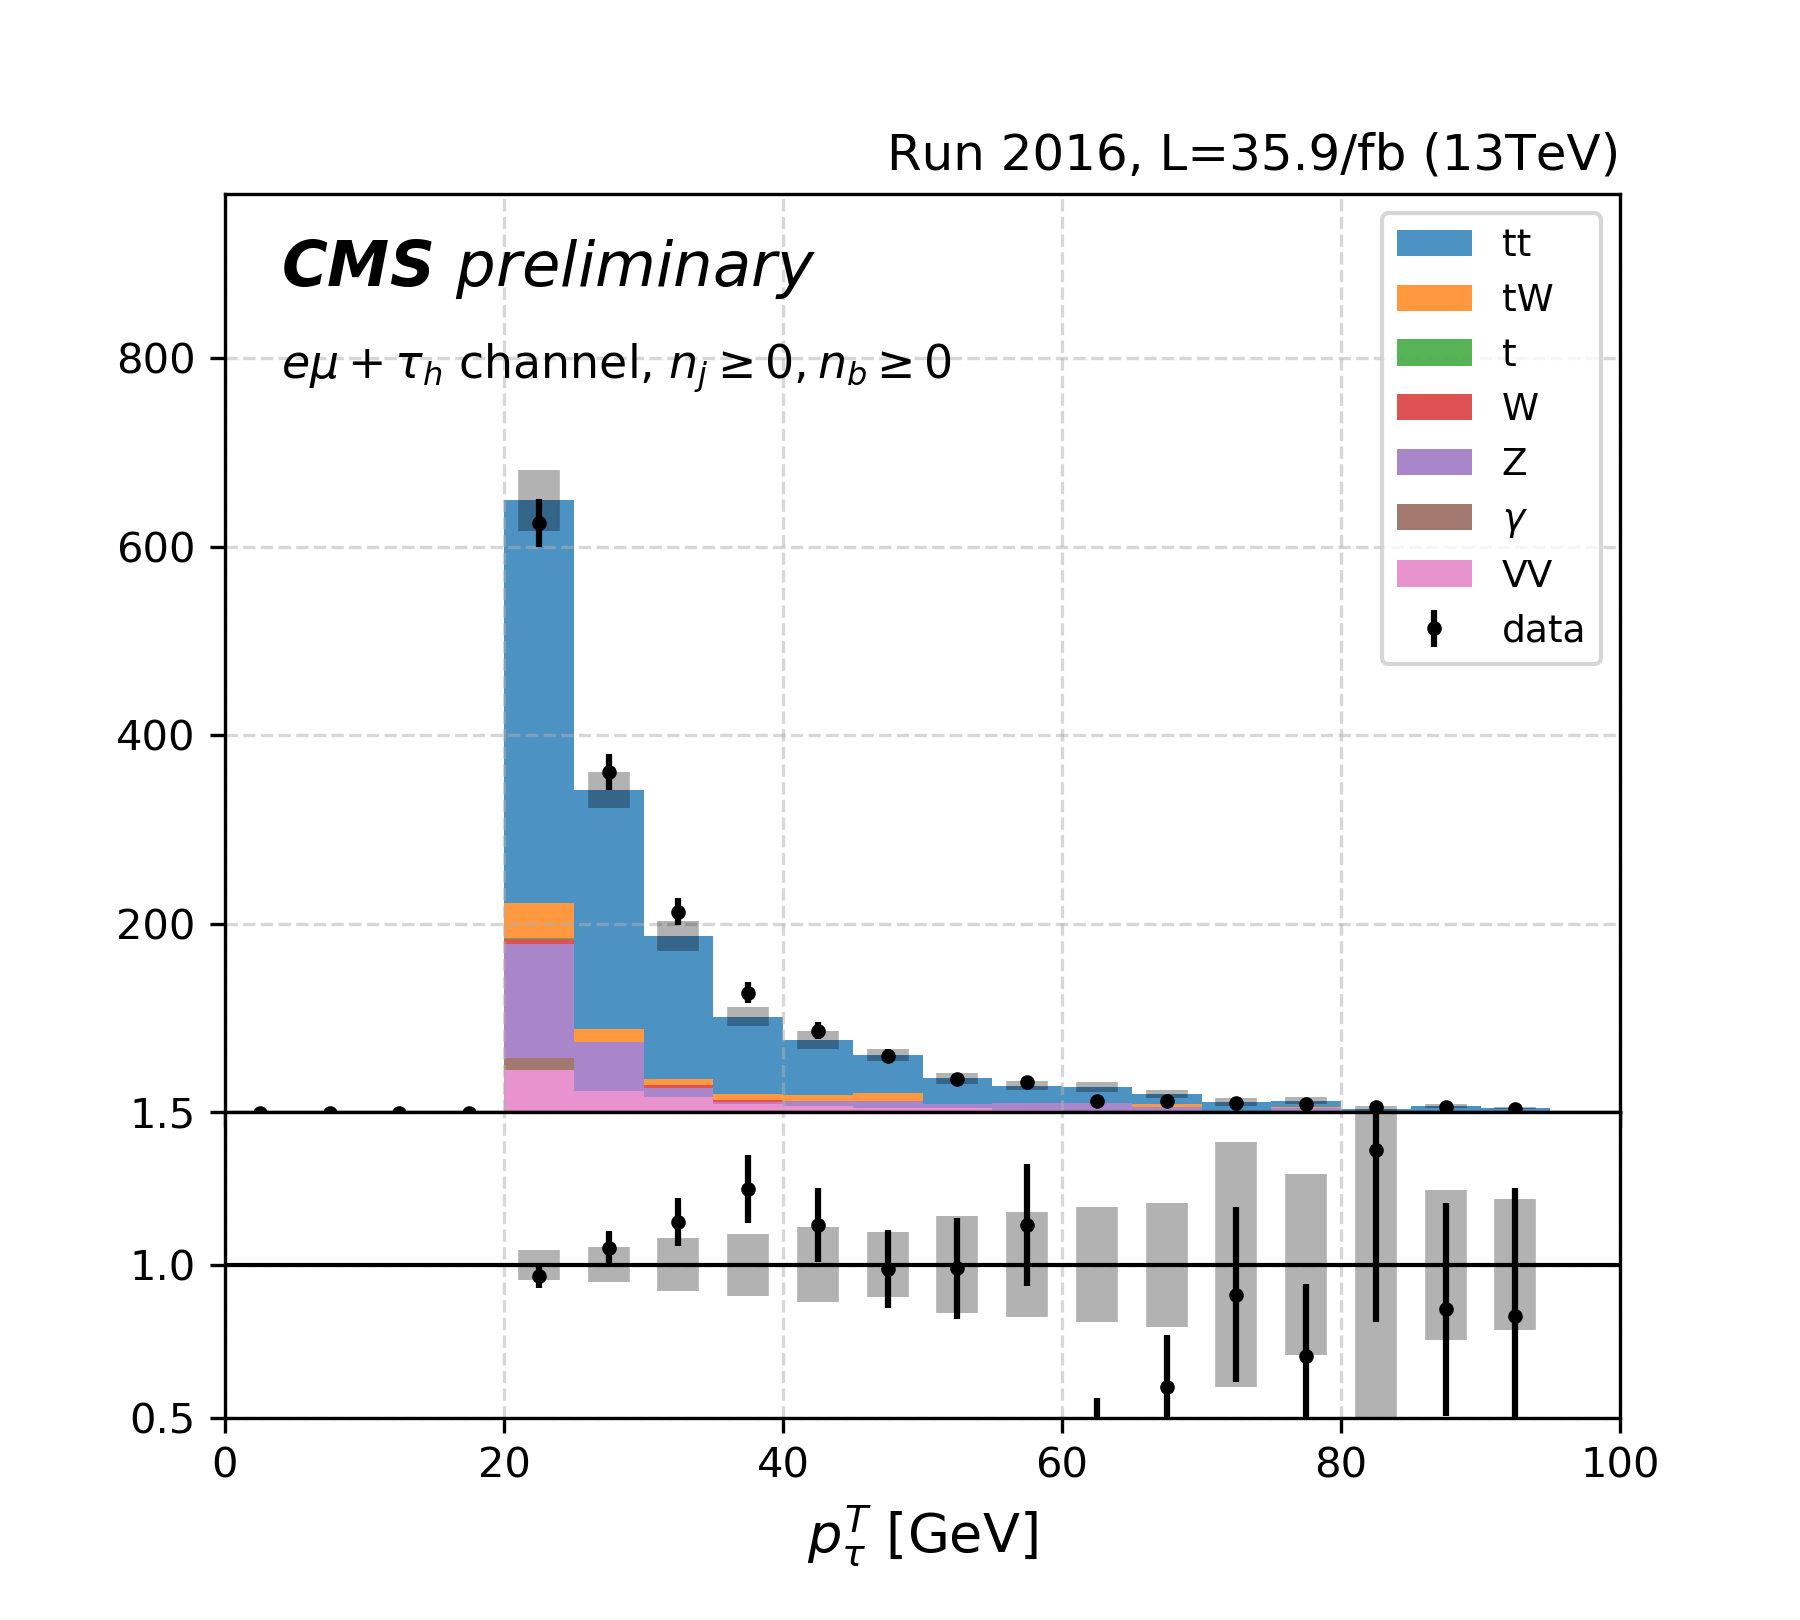
\includegraphics[width=0.4\textwidth]{chapters/Appendix/sectionJetToTauh/figures/emutau_tauPt_pickles_lltauVTight.png}
    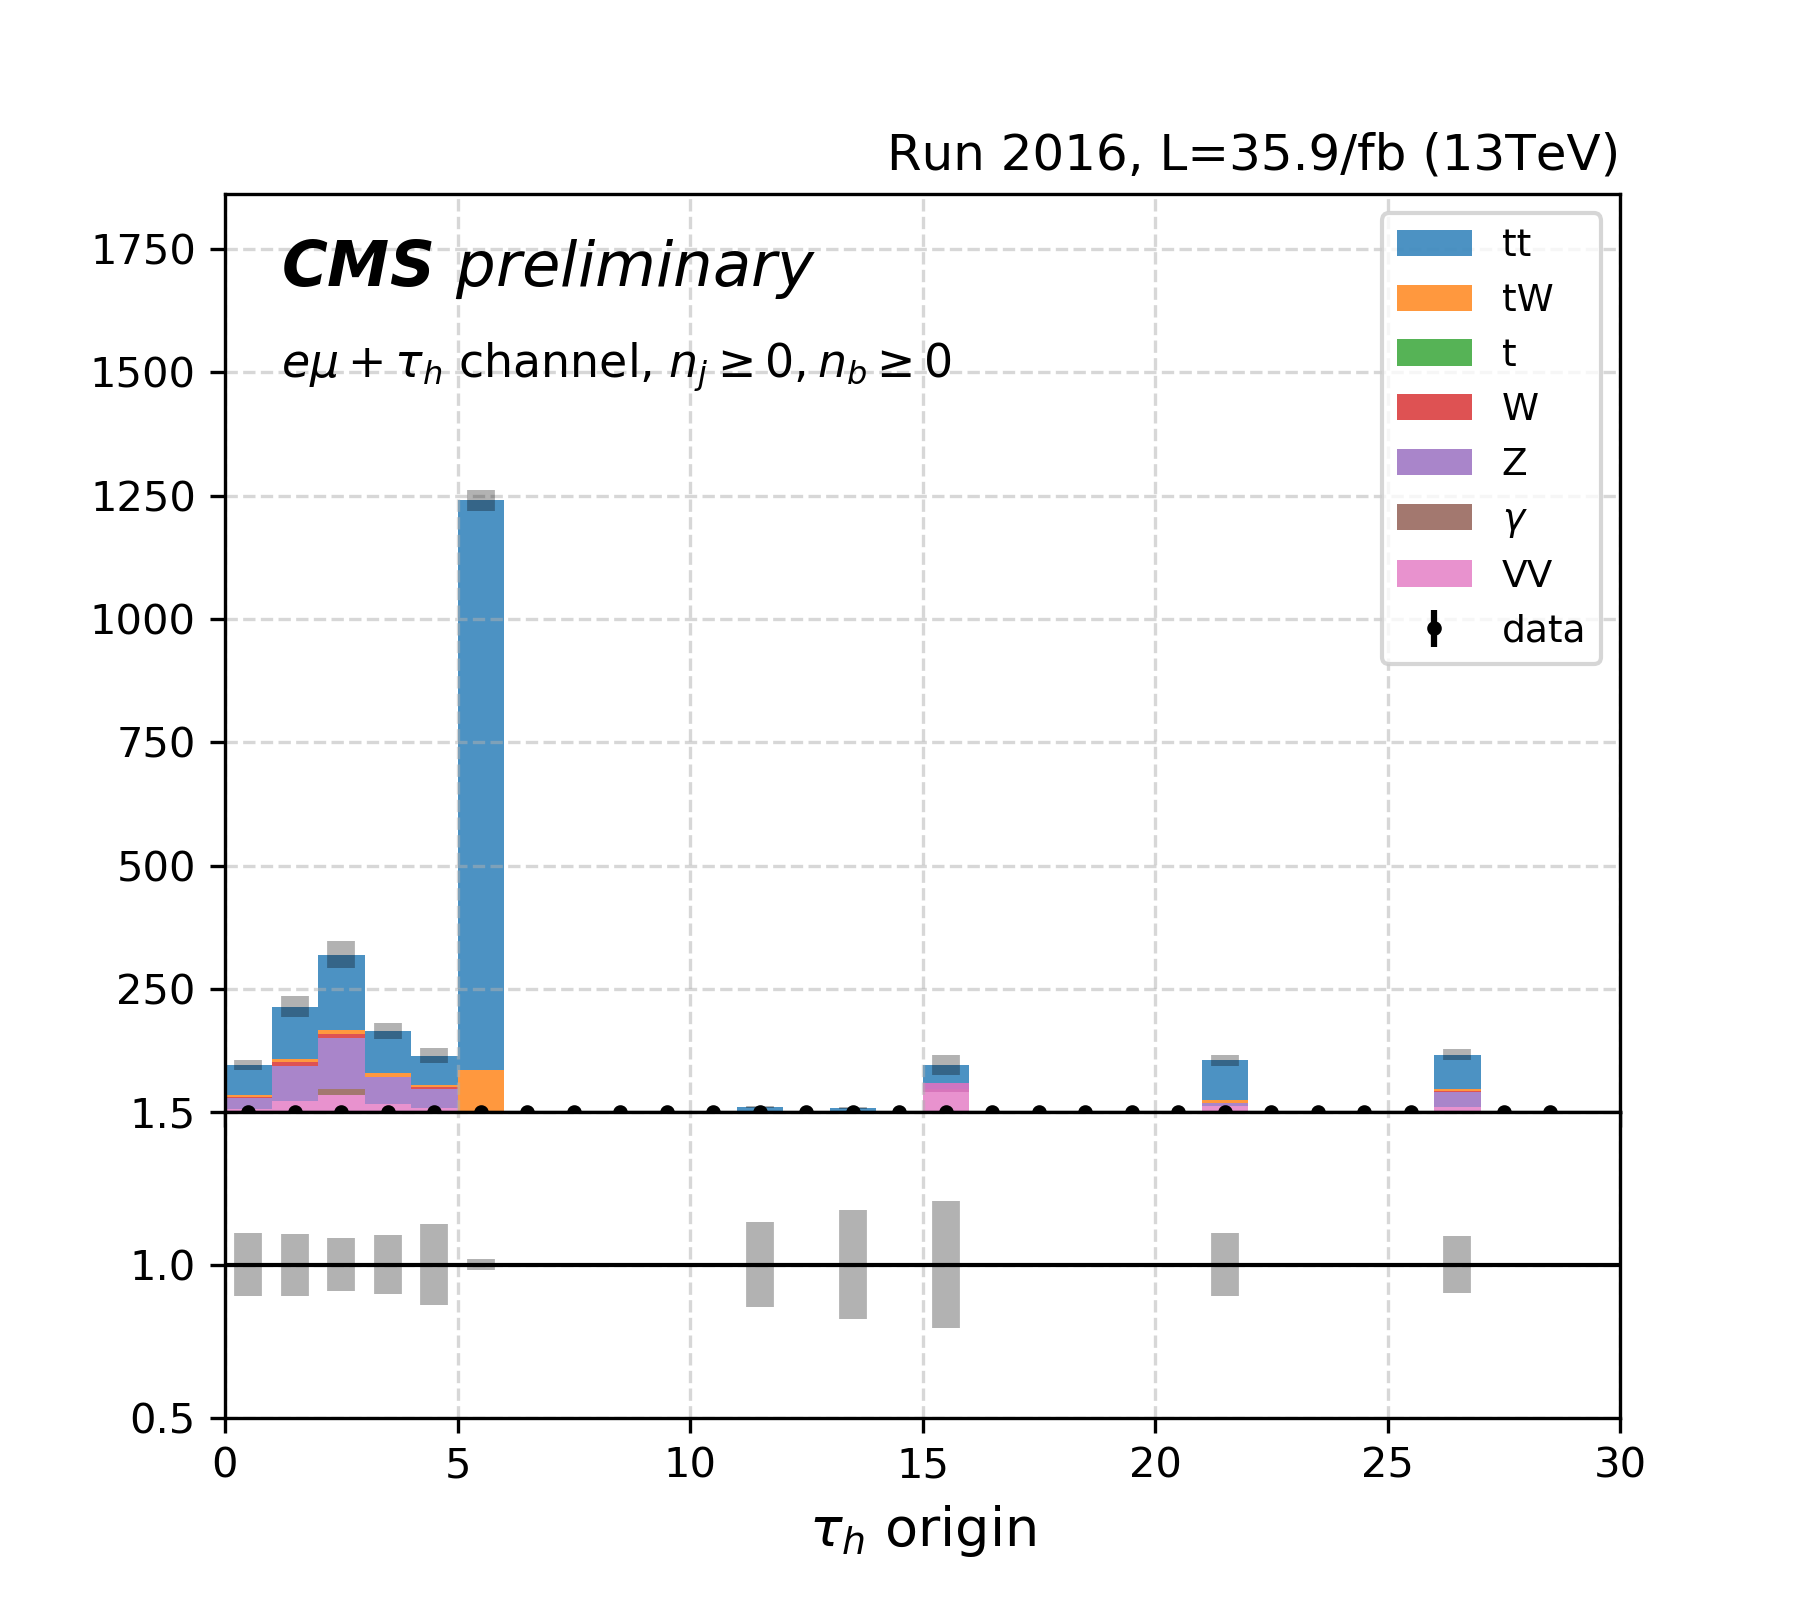
\includegraphics[width=0.4\textwidth]{chapters/Appendix/sectionJetToTauh/figures/emutau_tauGenFlavor_pickles_lltauTight.png}
    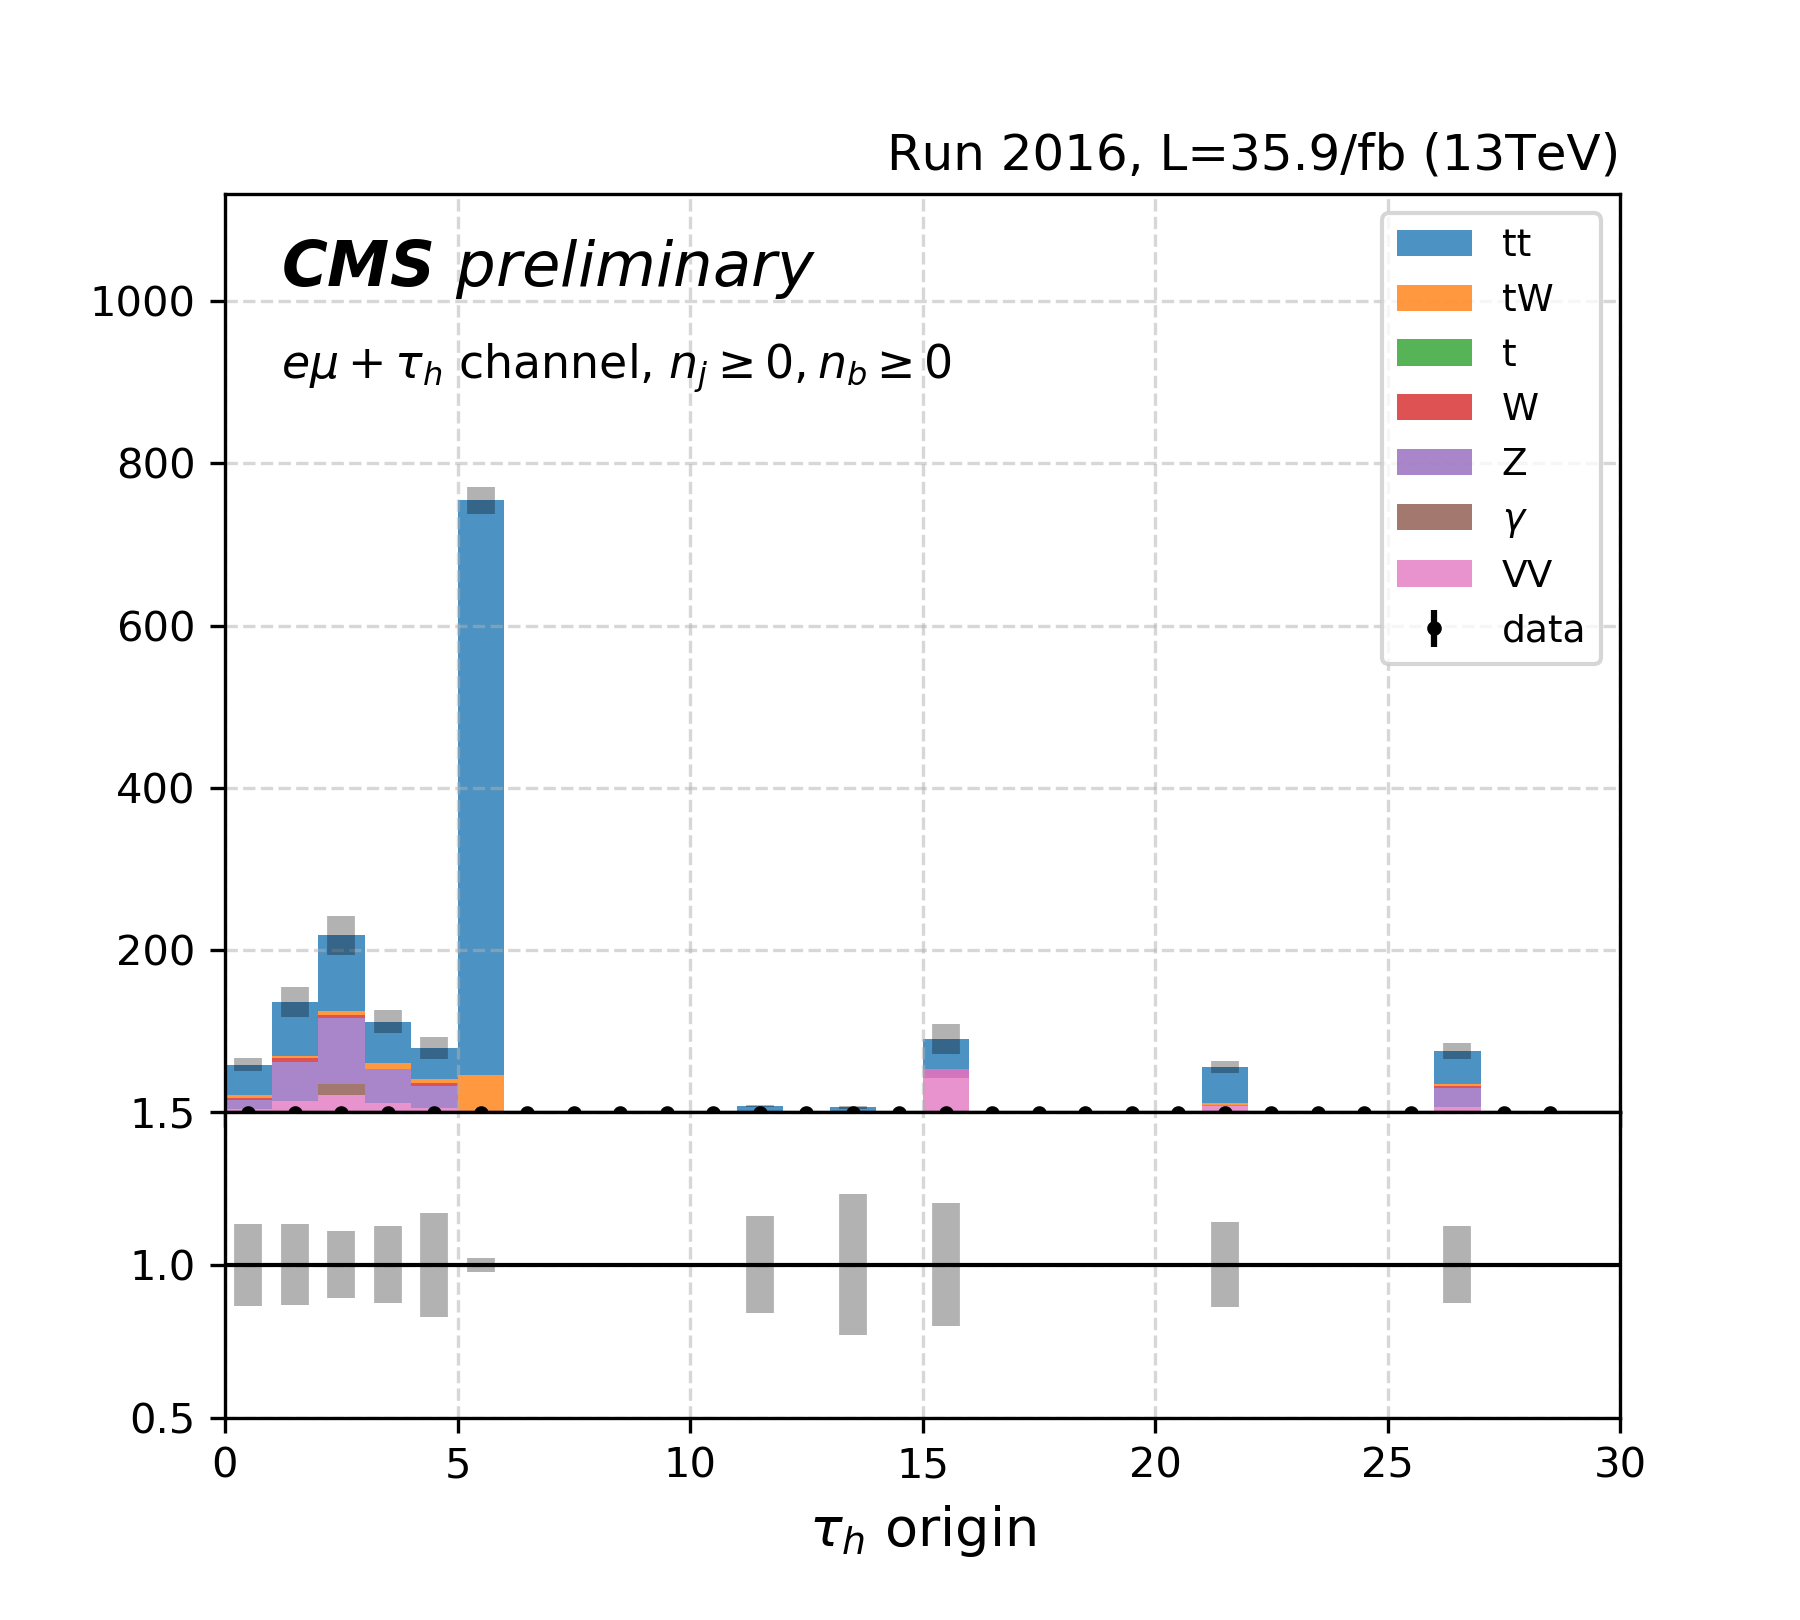
\includegraphics[width=0.4\textwidth]{chapters/Appendix/sectionJetToTauh/figures/emutau_tauGenFlavor_pickles_lltauVTight.png}
    \caption{Distributions of $m_{e\mu}$, $\tau pT$ and gen-level $\tau_h$ origin in the $e\mu+\tau$ channel. The left and right column shows the Tight and VTight $\tau_h$ WP respectively.}
    \label{fig:appendix:fakeTauId:emutau}
\end{figure}

\begin{figure}
    \centering
    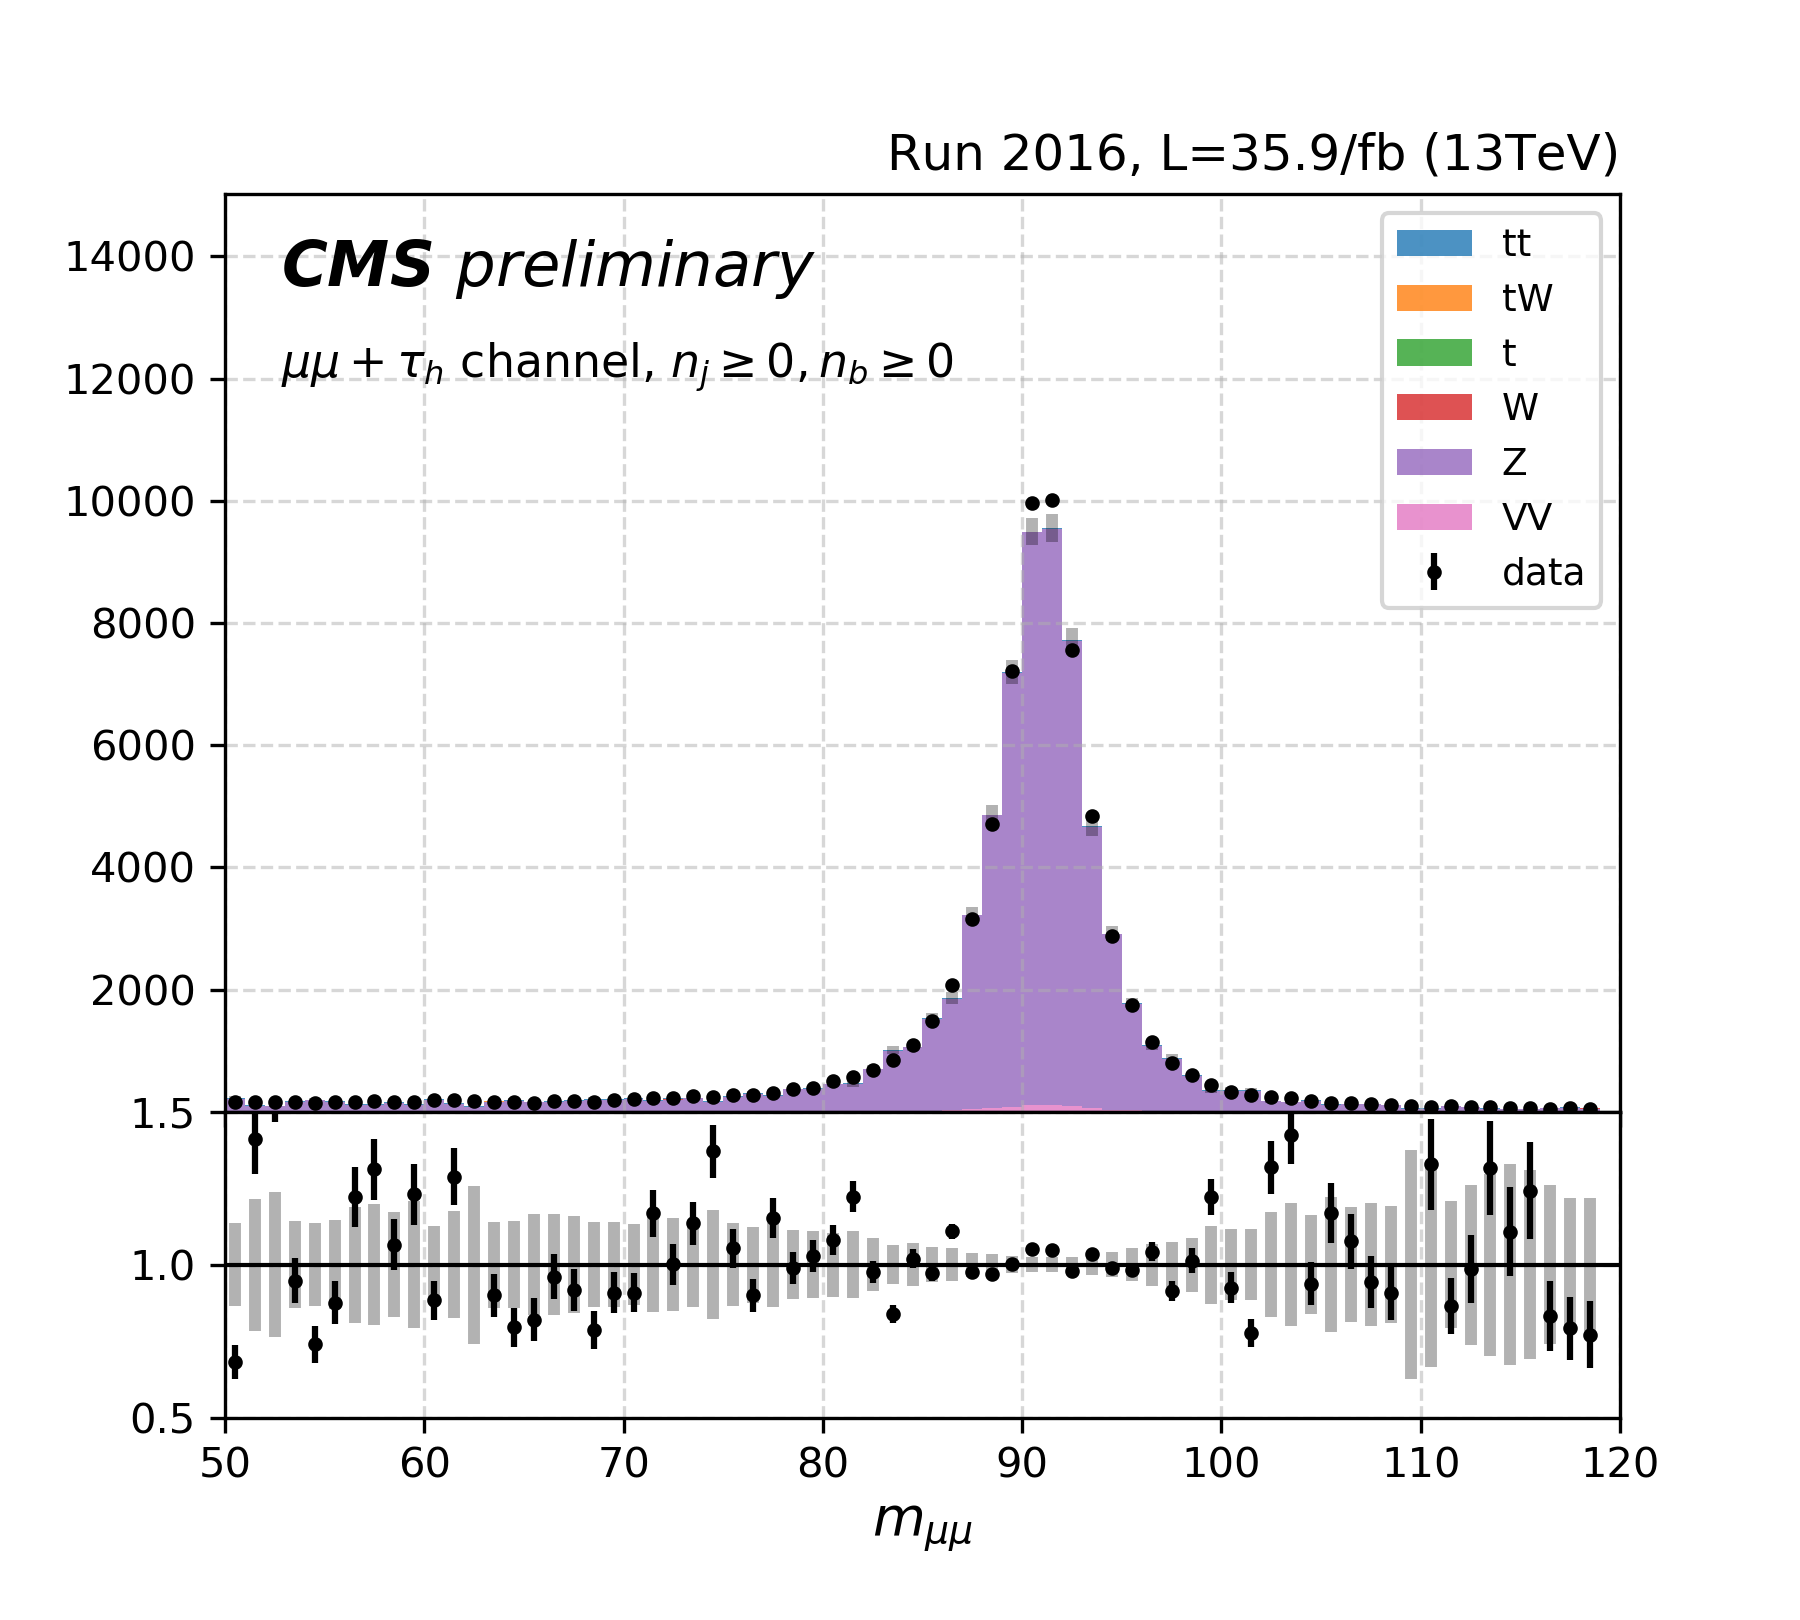
\includegraphics[width=0.4\textwidth]{chapters/Appendix/sectionJetToTauh/figures/mumutau_dilepton_mass_pickles_lltauTight.png}
    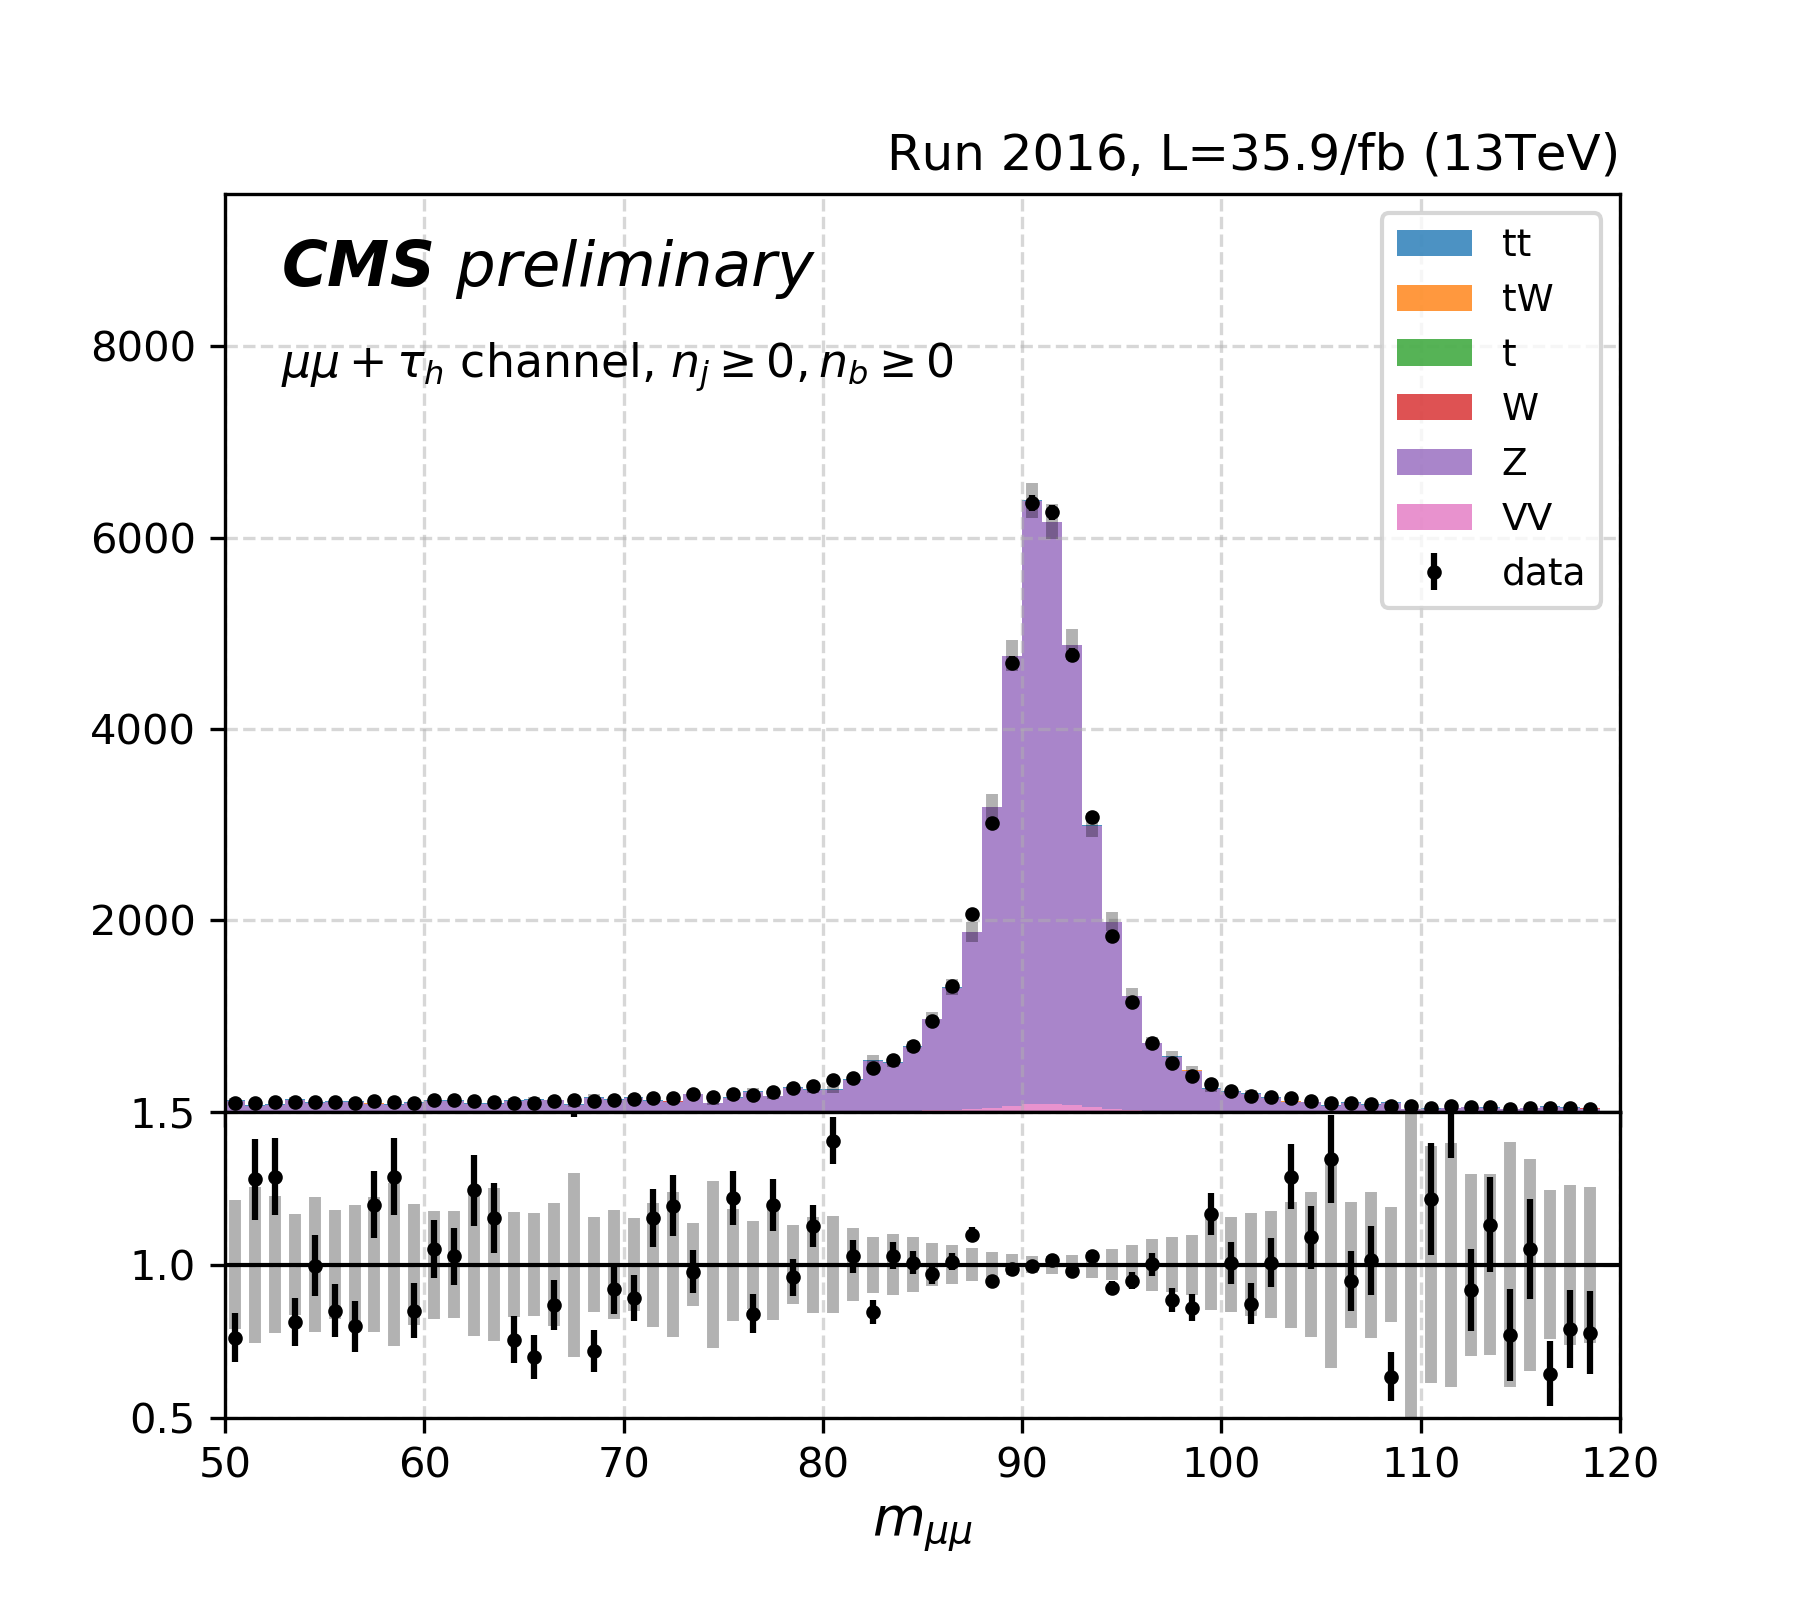
\includegraphics[width=0.4\textwidth]{chapters/Appendix/sectionJetToTauh/figures/mumutau_dilepton_mass_pickles_lltauVTight.png}
    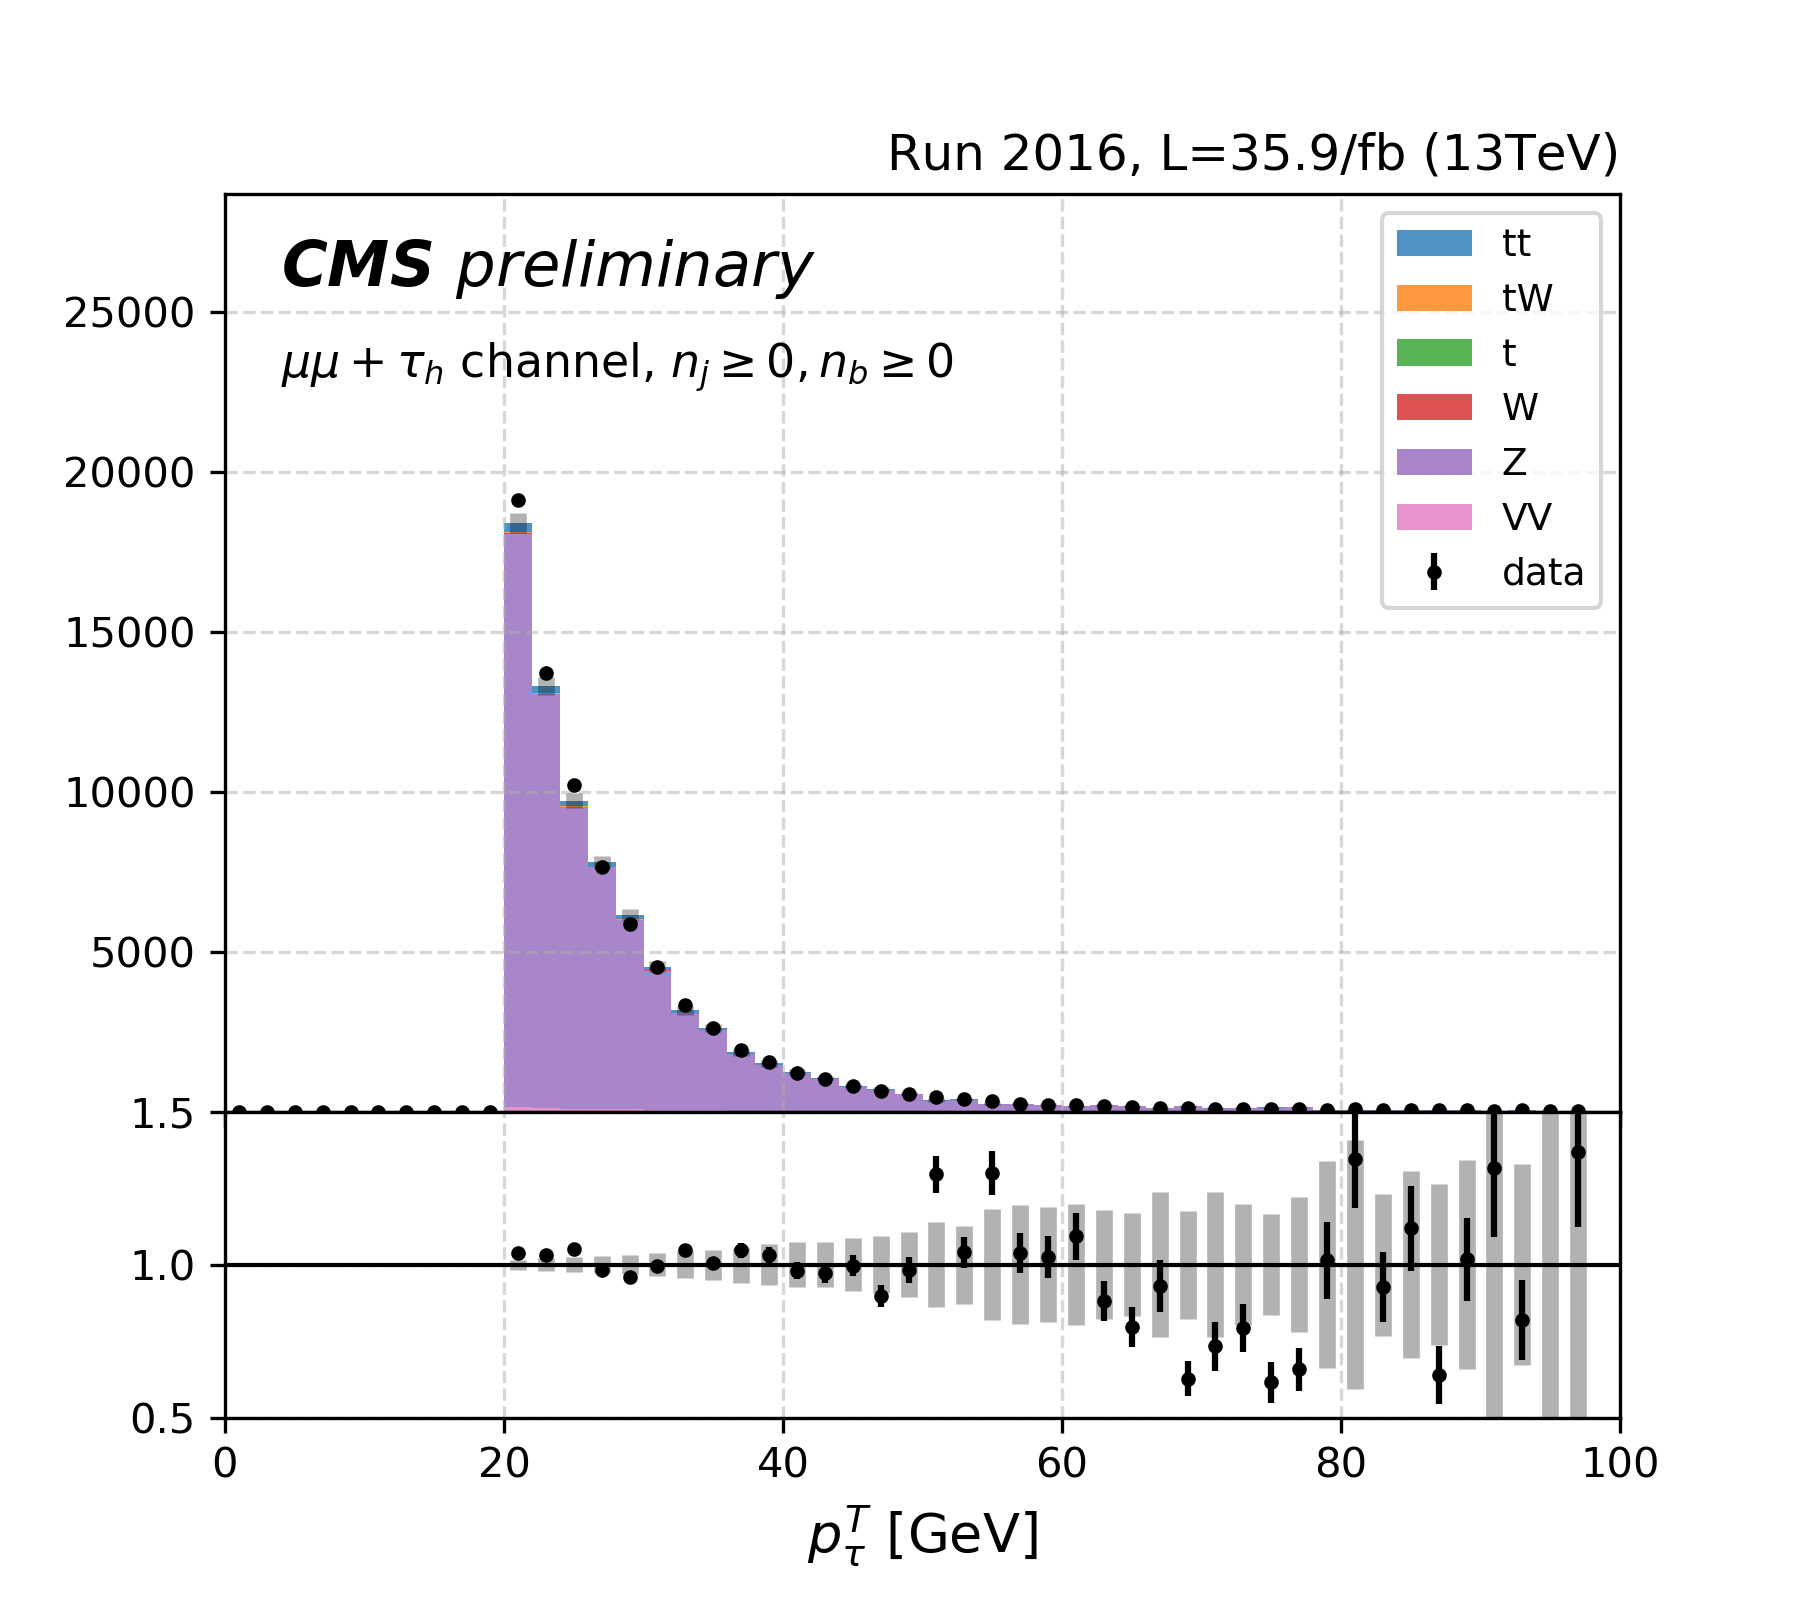
\includegraphics[width=0.4\textwidth]{chapters/Appendix/sectionJetToTauh/figures/mumutau_tauPt_pickles_lltauTight.png}
    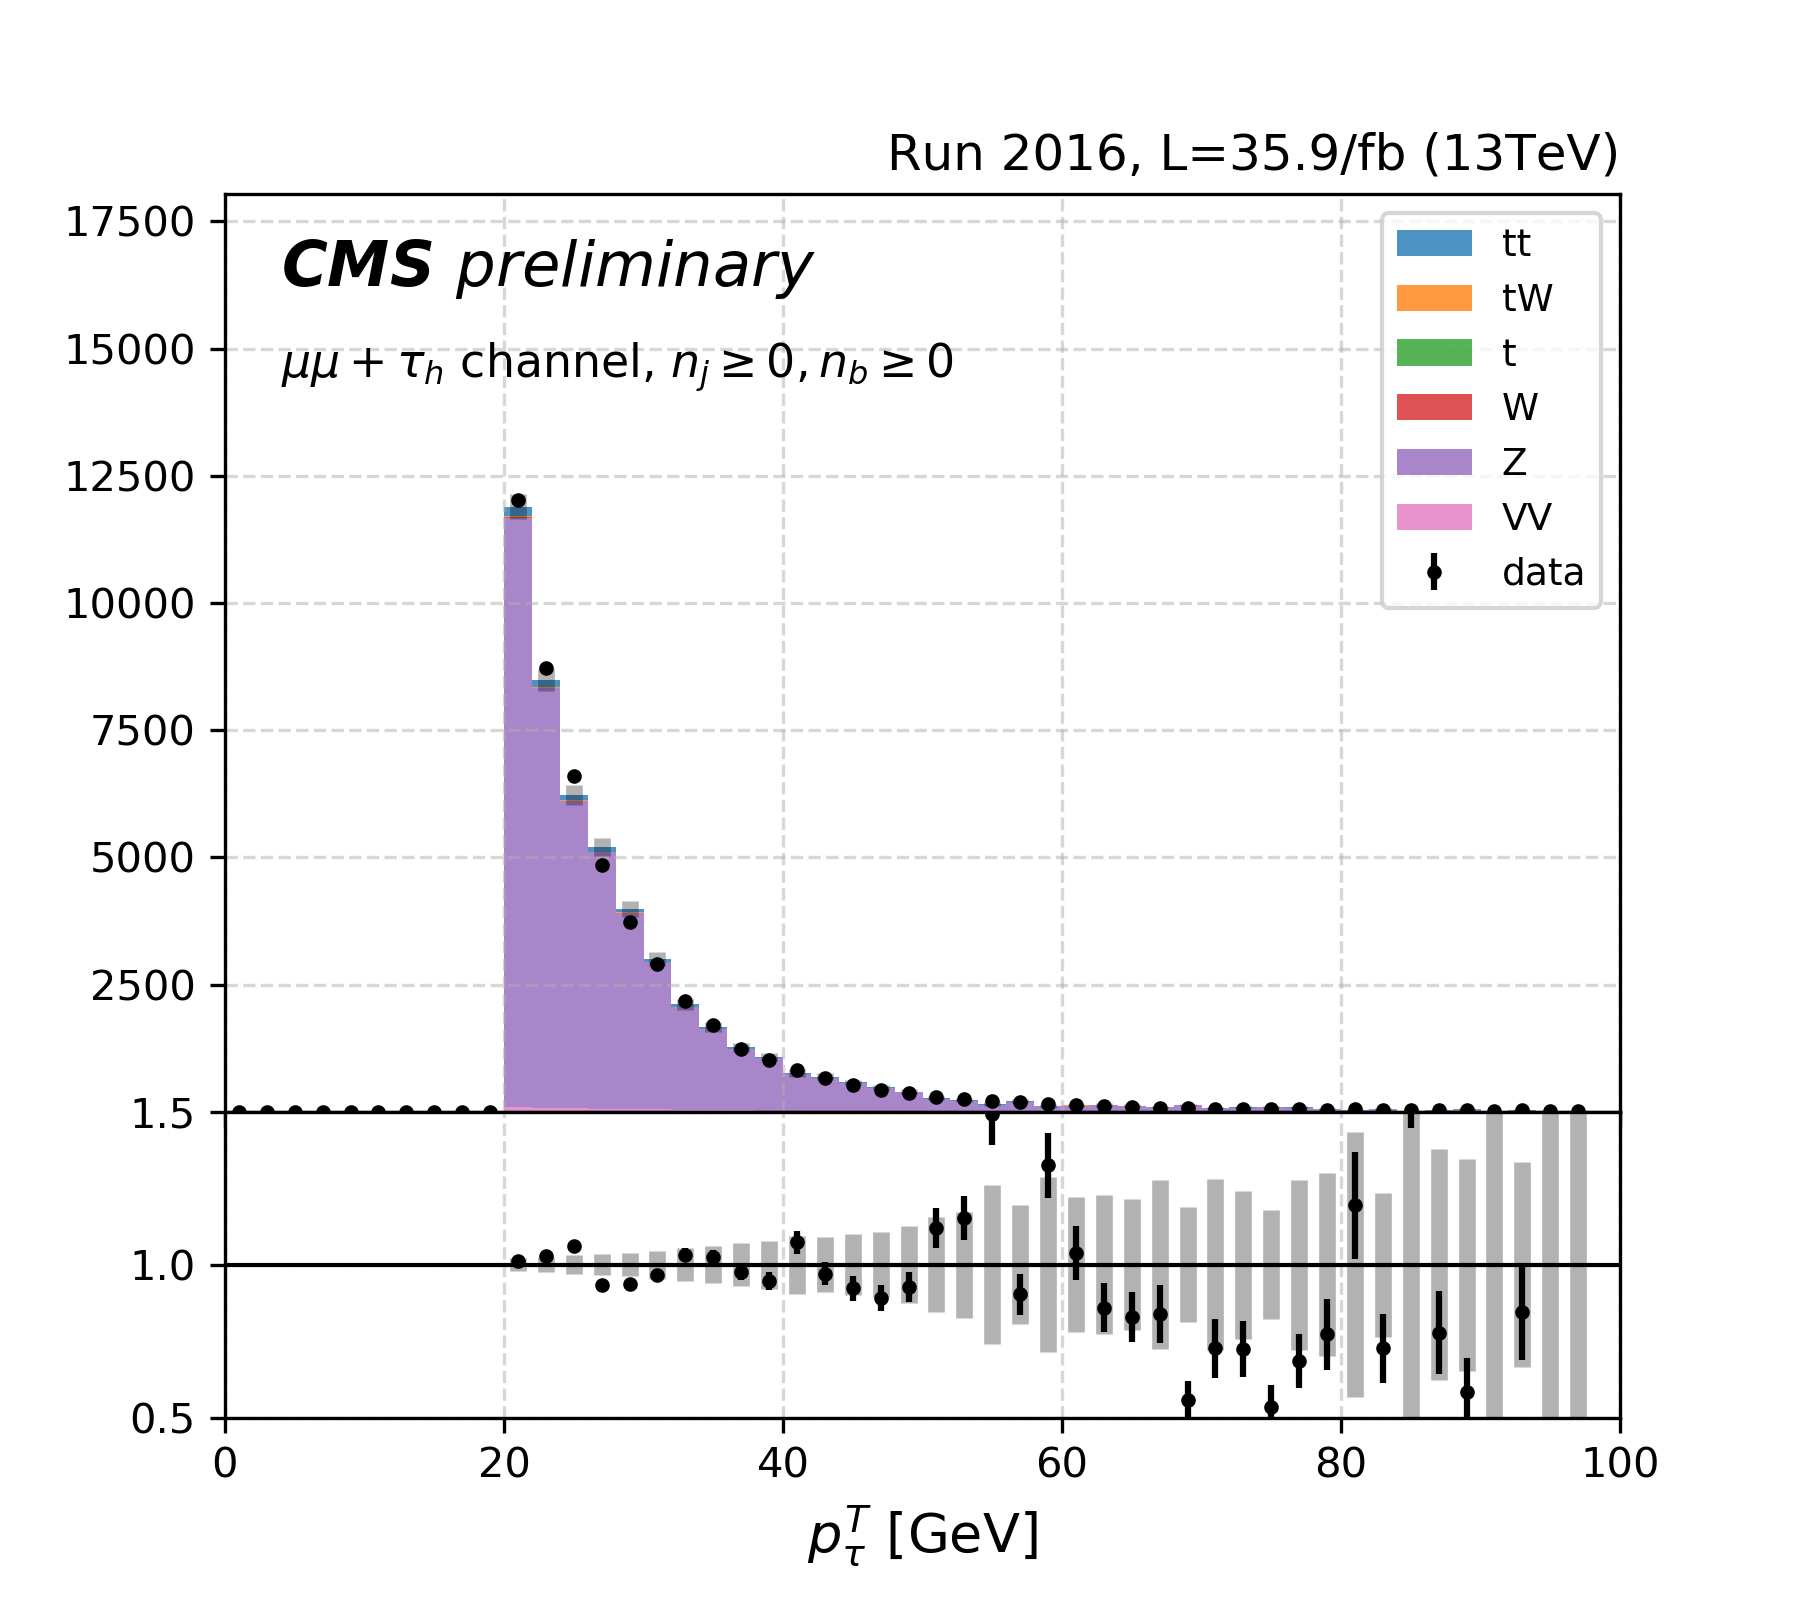
\includegraphics[width=0.4\textwidth]{chapters/Appendix/sectionJetToTauh/figures/mumutau_tauPt_pickles_lltauVTight.png}
    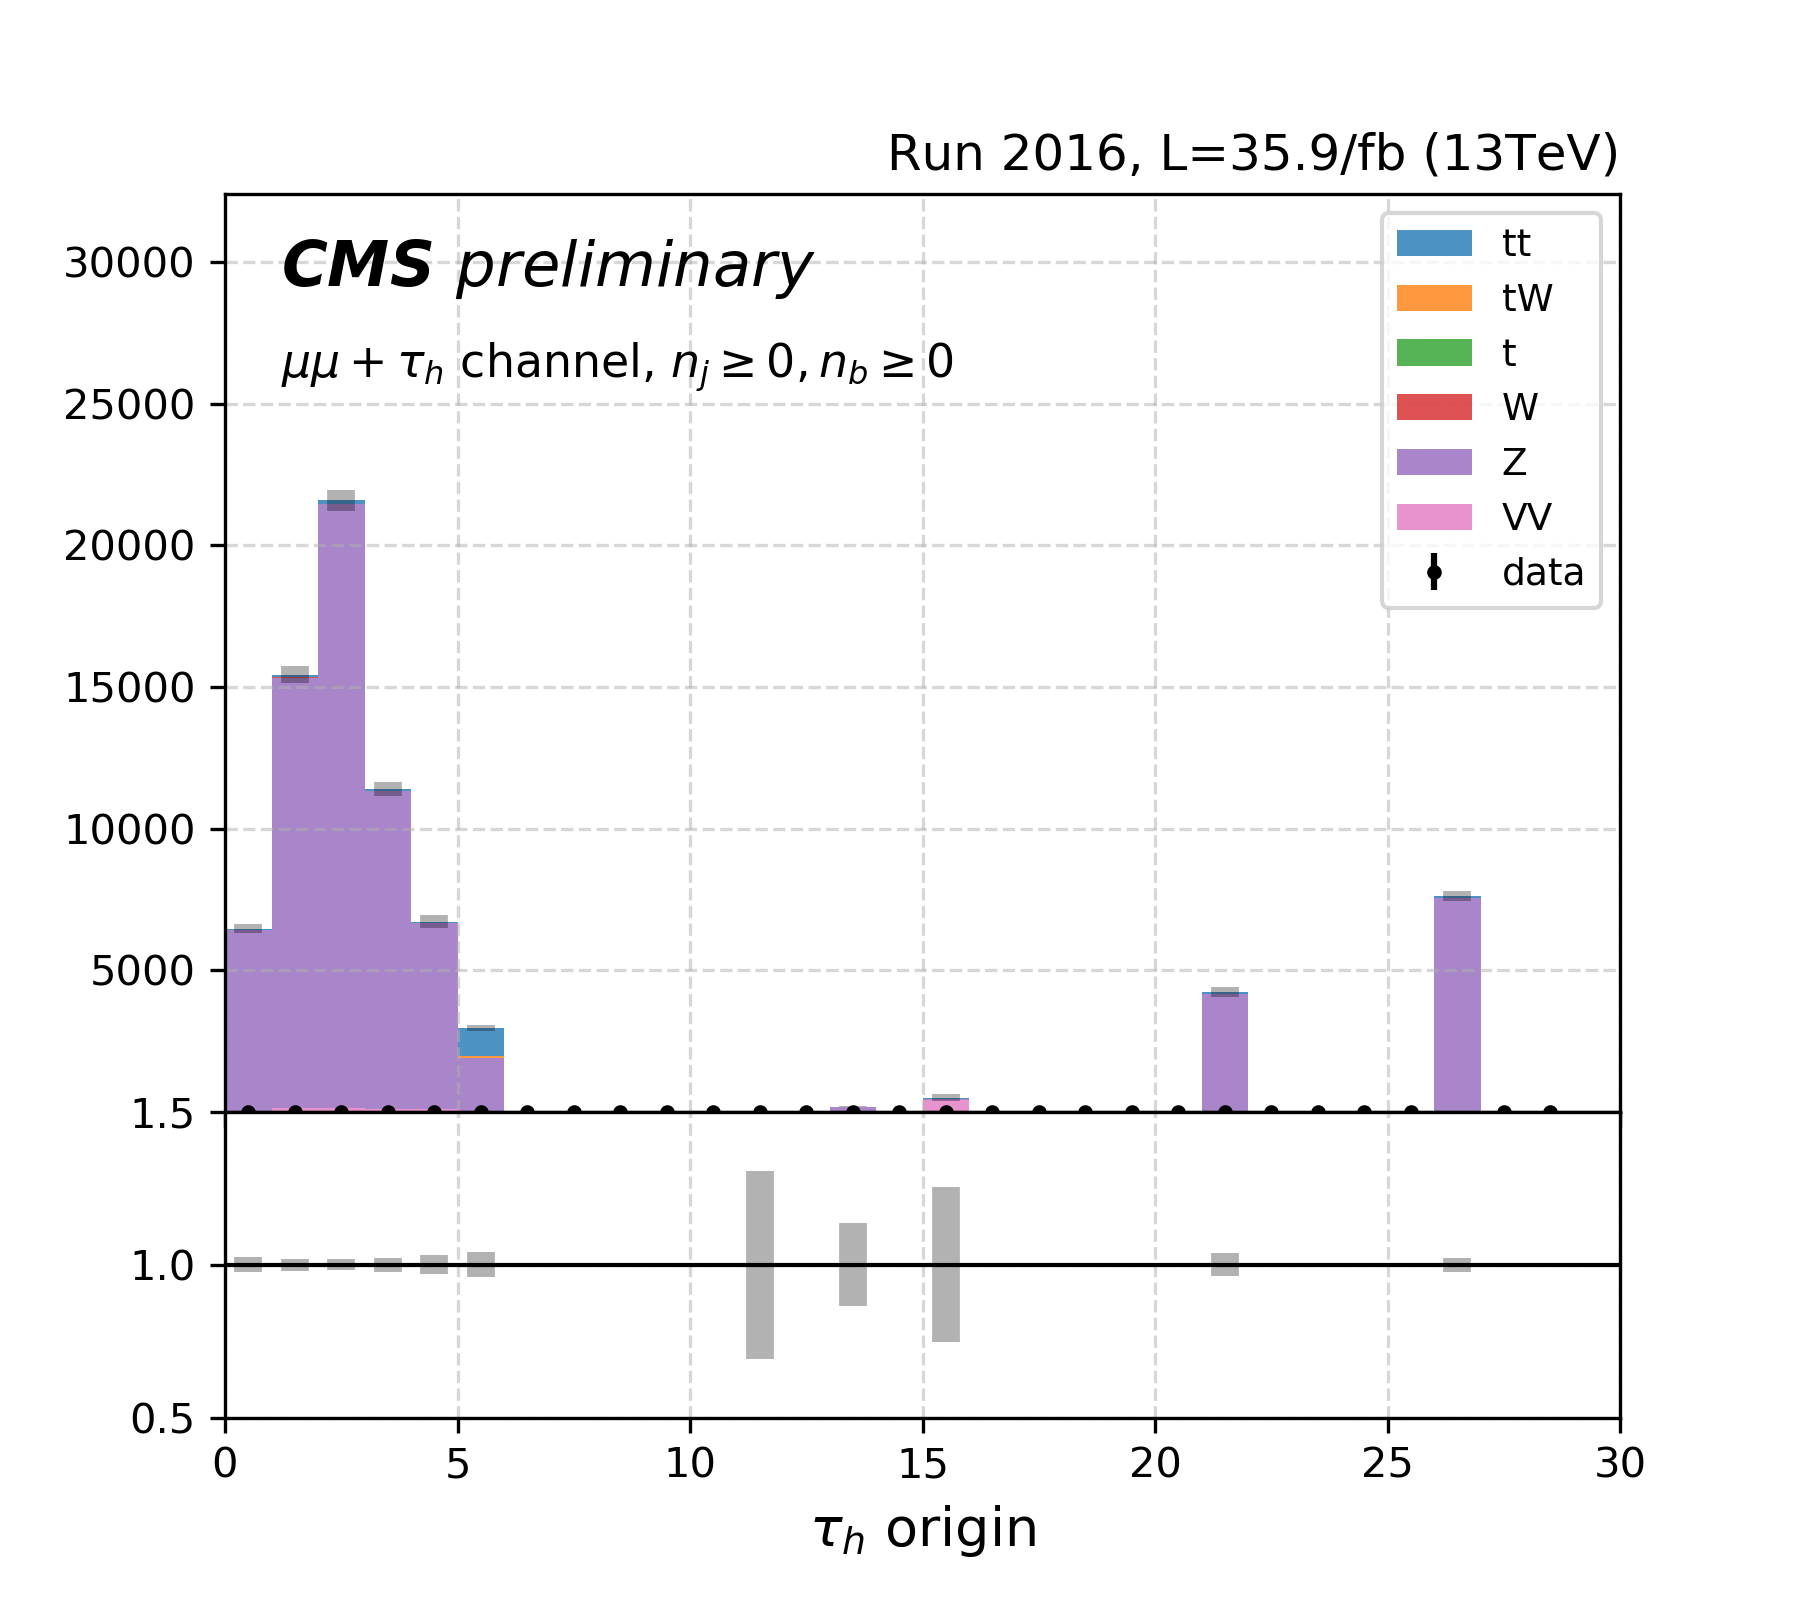
\includegraphics[width=0.4\textwidth]{chapters/Appendix/sectionJetToTauh/figures/mumutau_tauGenFlavor_pickles_lltauTight.png}
    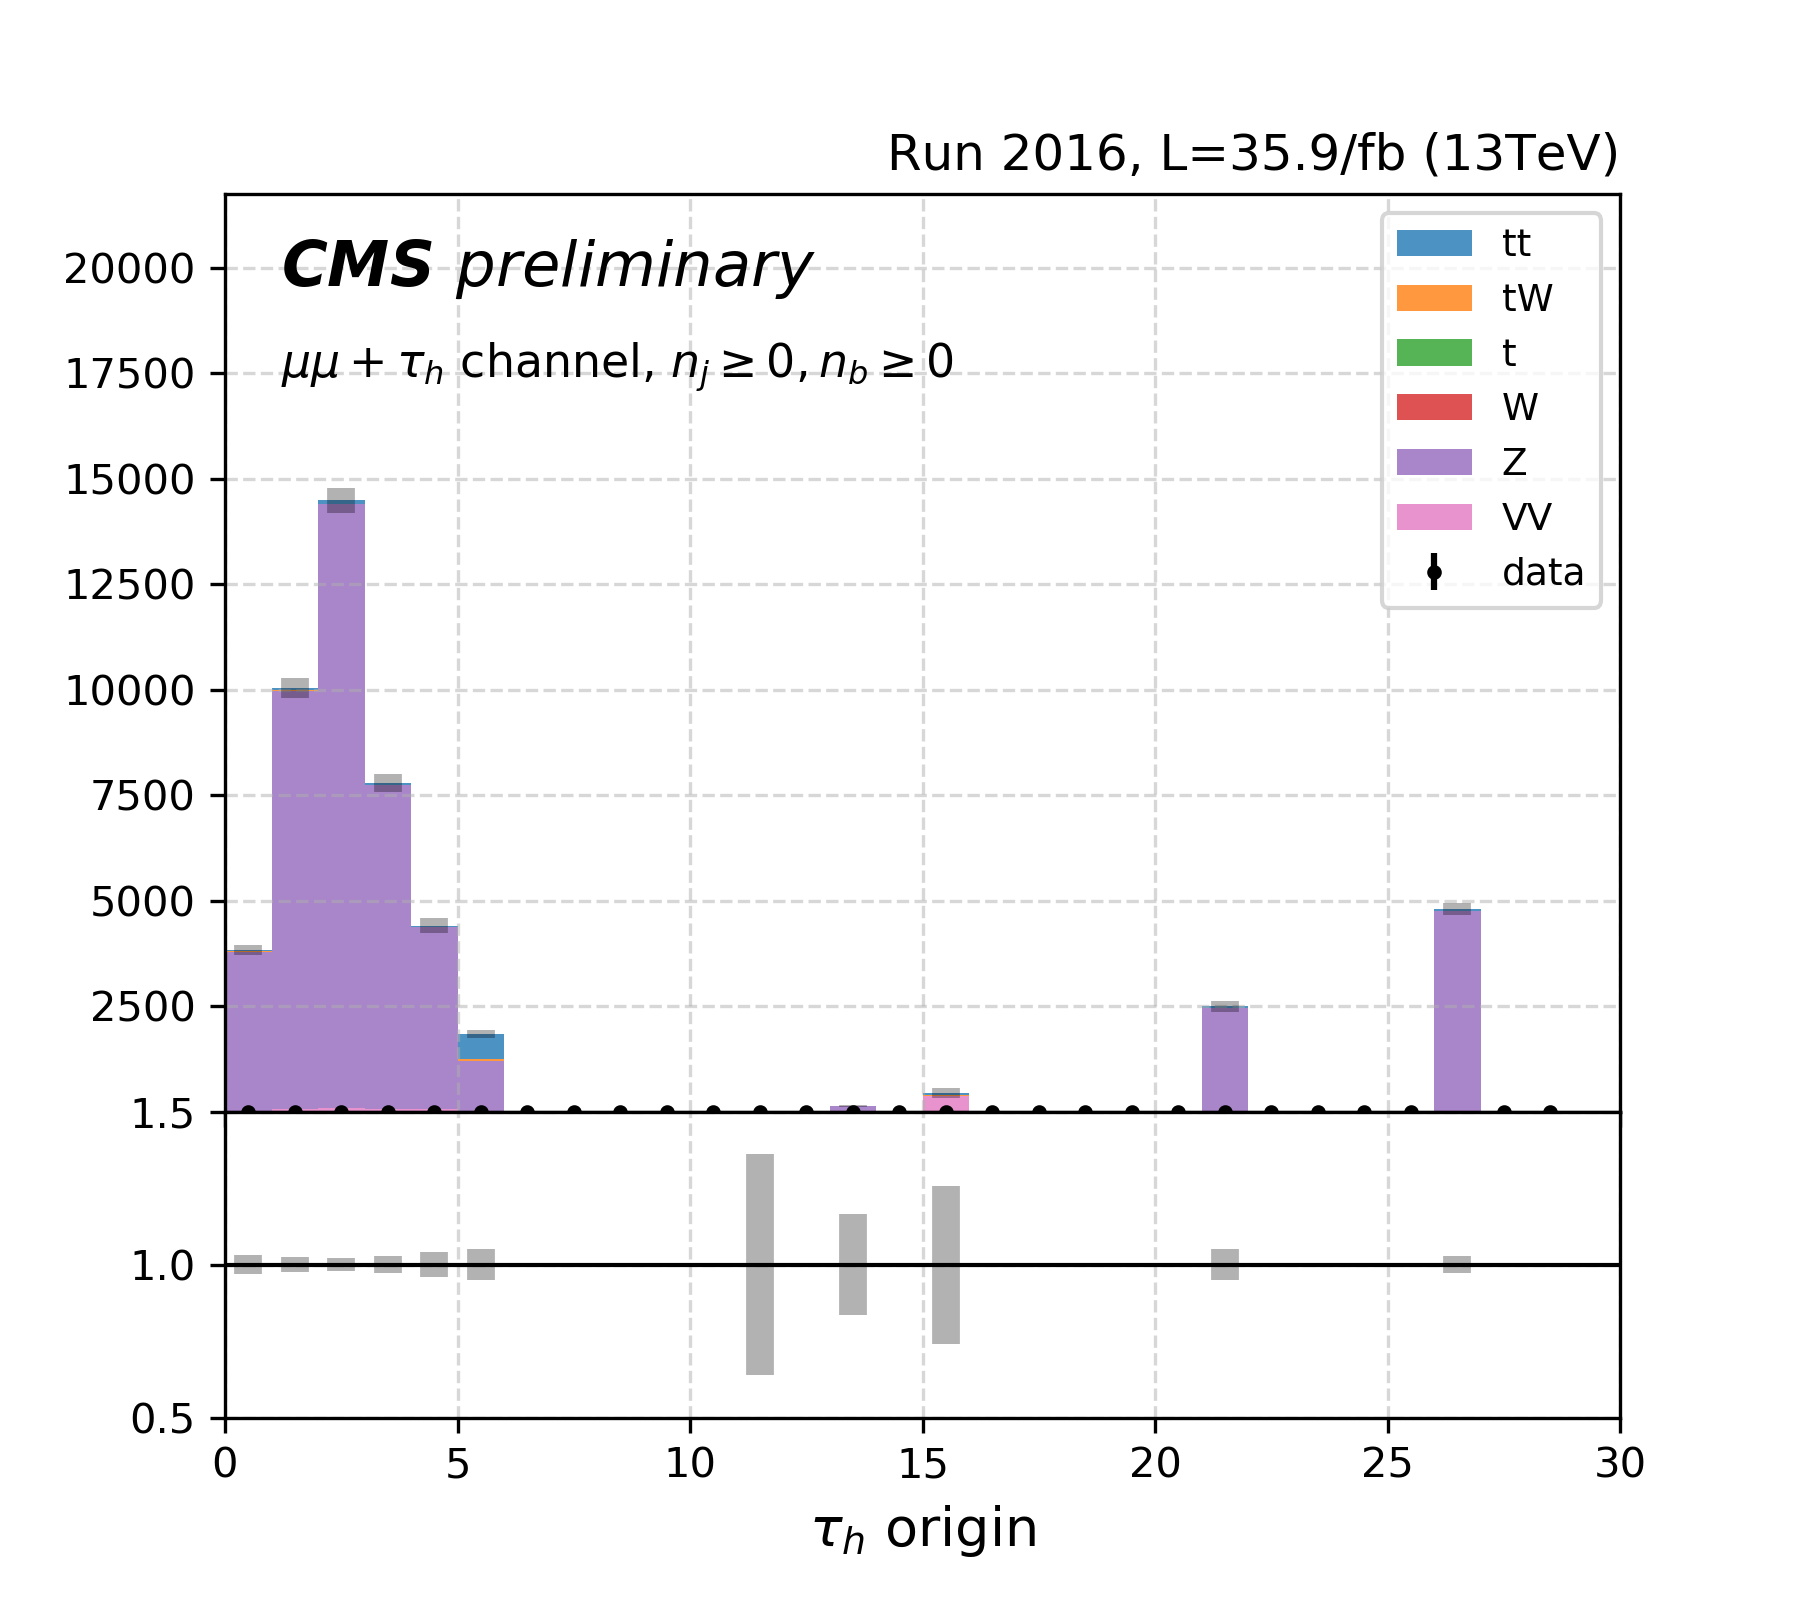
\includegraphics[width=0.4\textwidth]{chapters/Appendix/sectionJetToTauh/figures/mumutau_tauGenFlavor_pickles_lltauVTight.png}
    \caption{Distributions of $m_{\mu\mu}$, $\tau pT$ and gen-level $\tau_h$ origin in the $\mu\mu+\tau$ channel. The left and right column shows the Tight and VTight $\tau_h$ WP respectively.}
    \label{fig:appendix:fakeTauId:mumutau}
\end{figure}


\begin{figure}
    \centering
    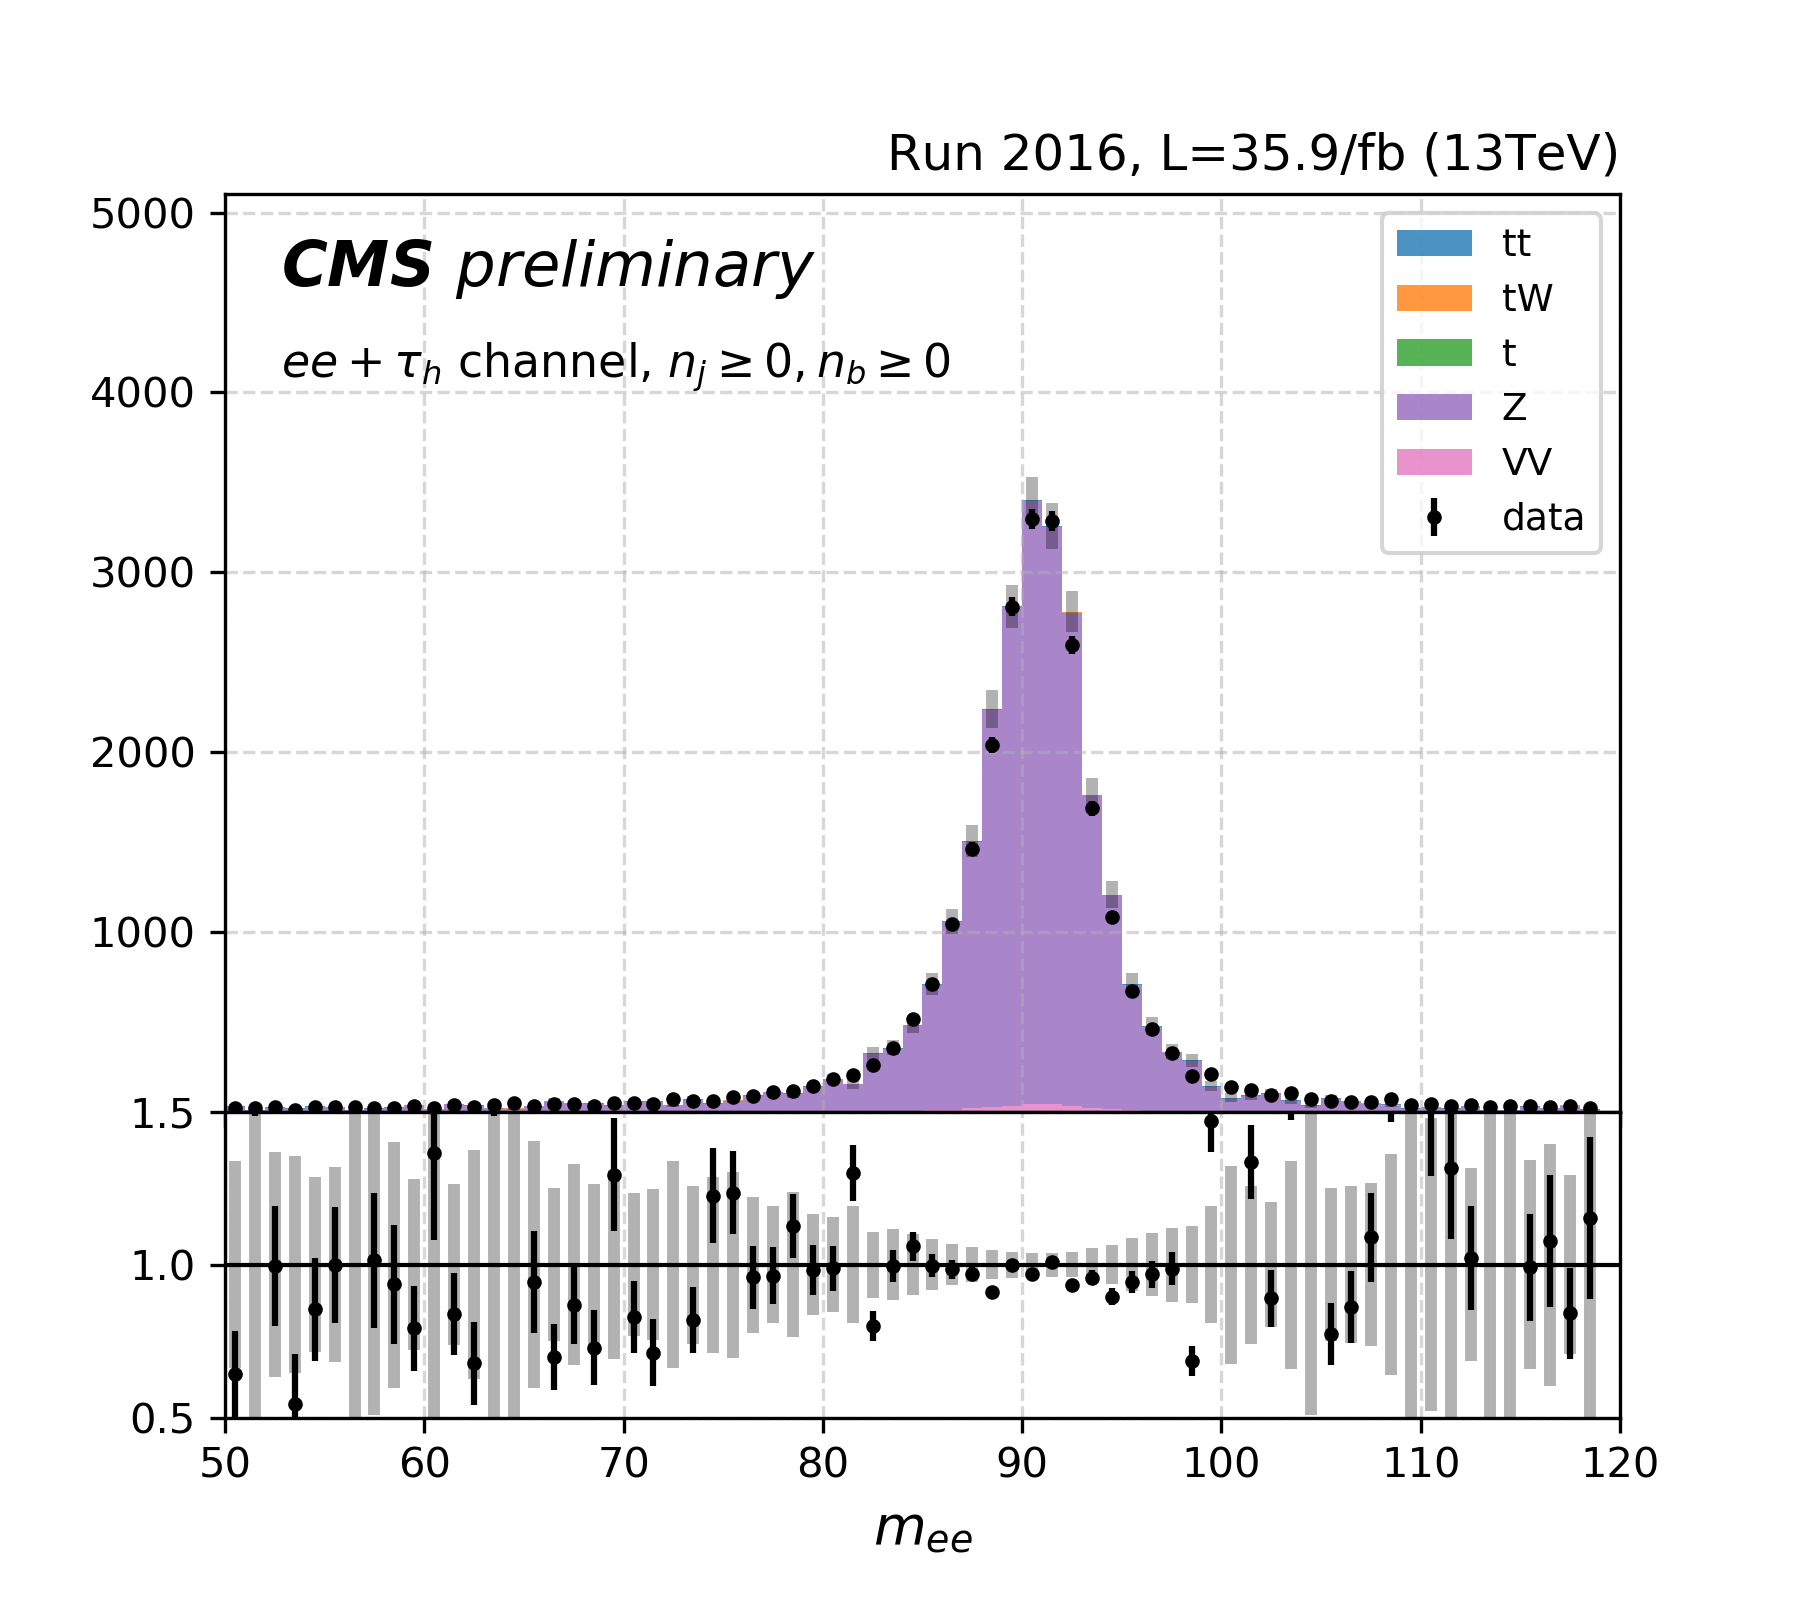
\includegraphics[width=0.4\textwidth]{chapters/Appendix/sectionJetToTauh/figures/eetau_dilepton_mass_pickles_lltauTight.png}
    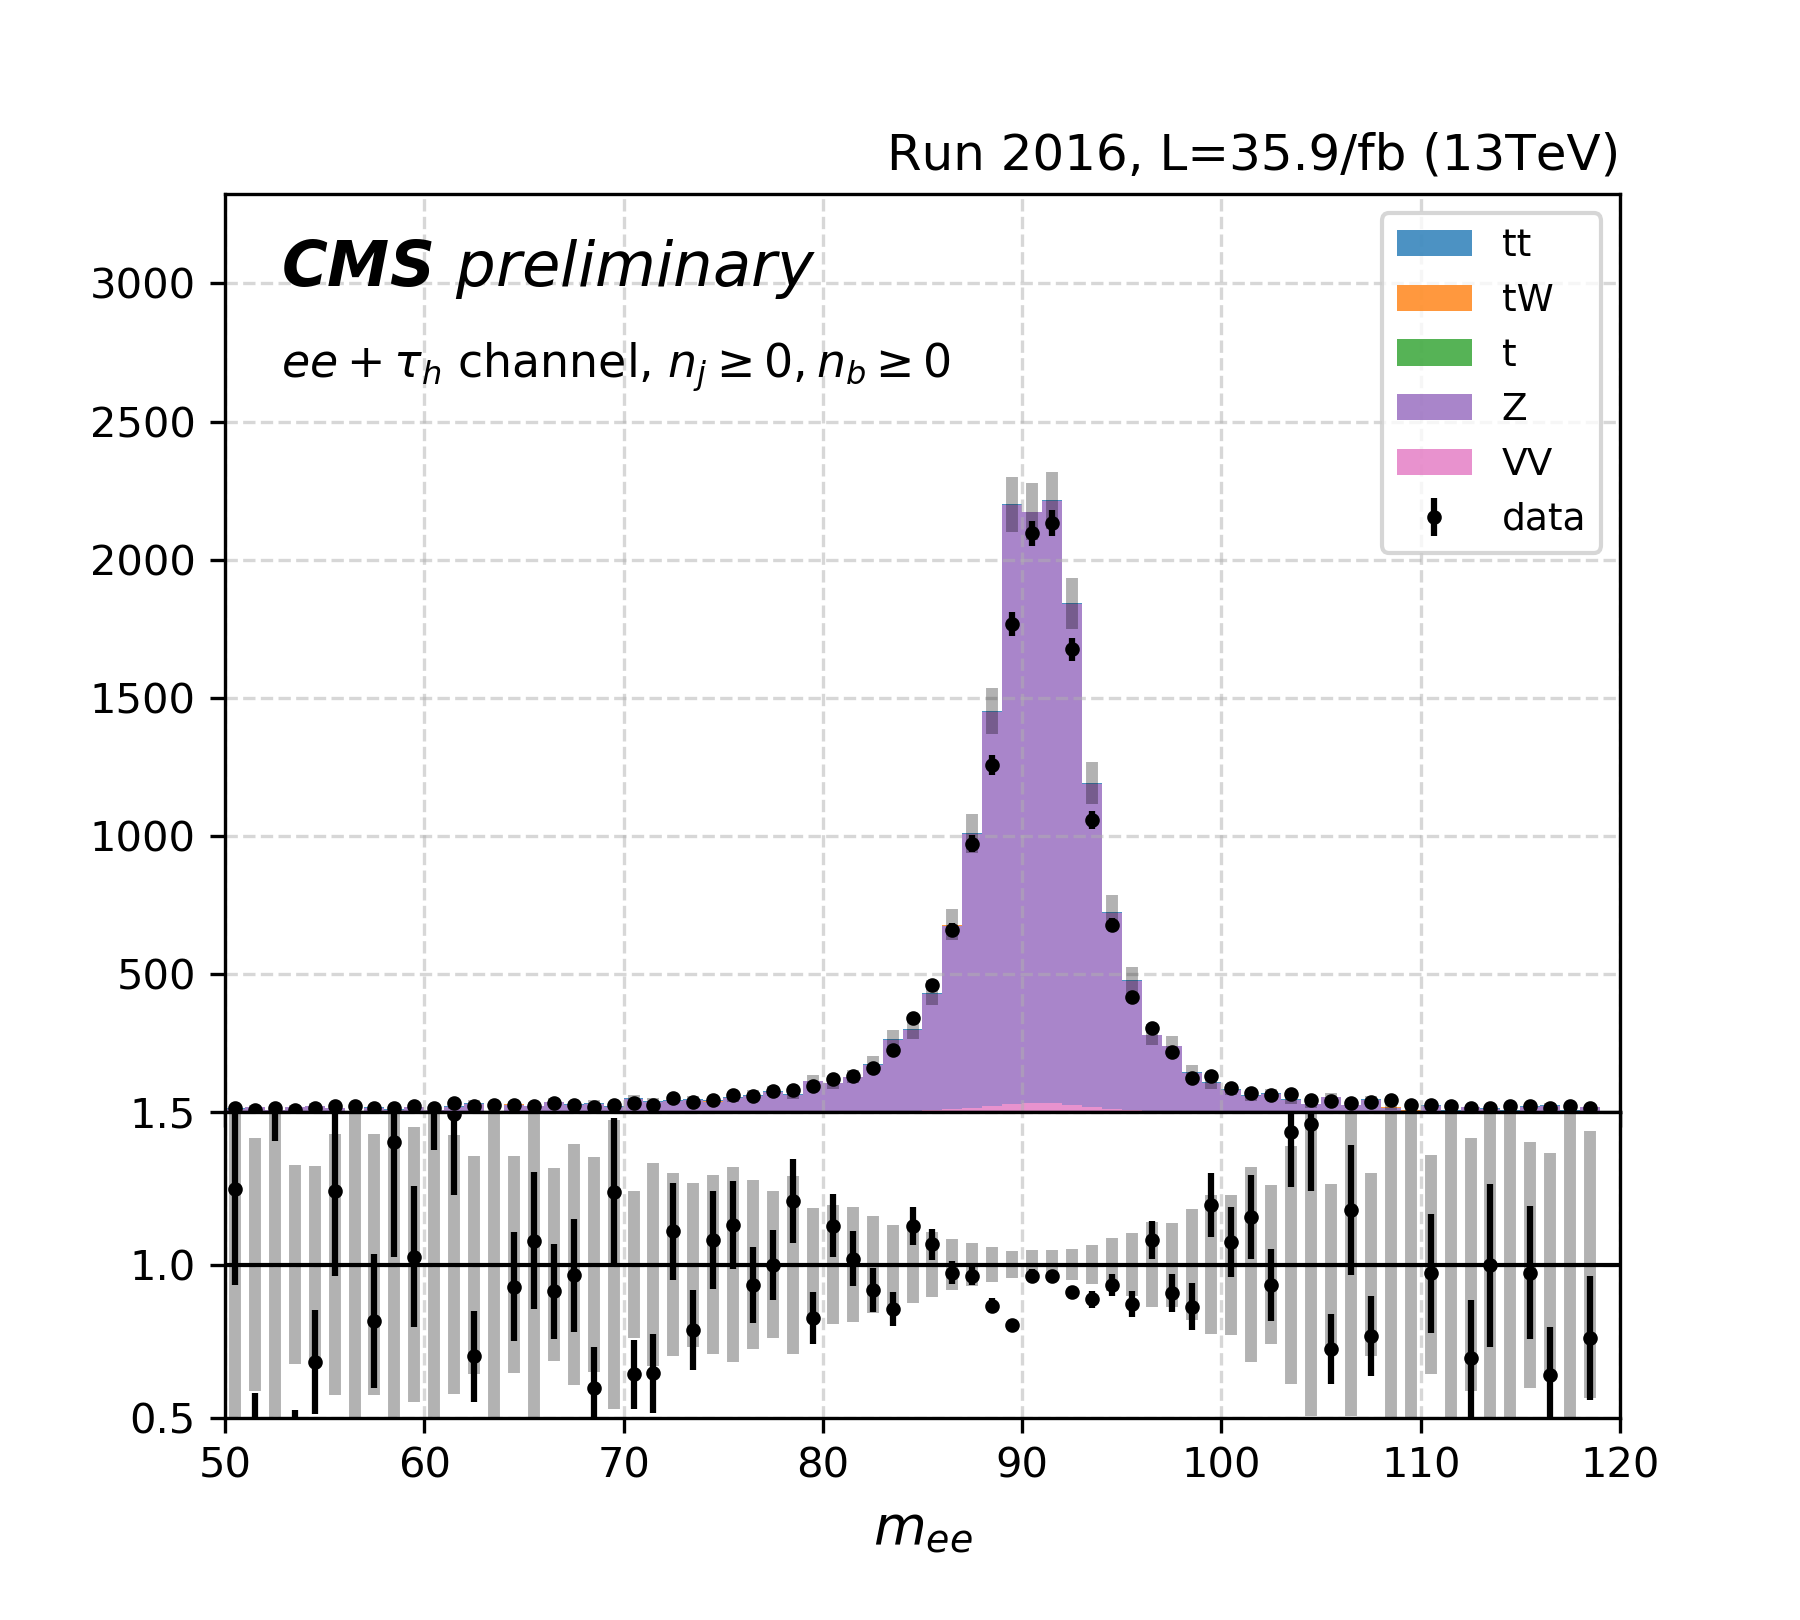
\includegraphics[width=0.4\textwidth]{chapters/Appendix/sectionJetToTauh/figures/eetau_dilepton_mass_pickles_lltauVTight.png}
    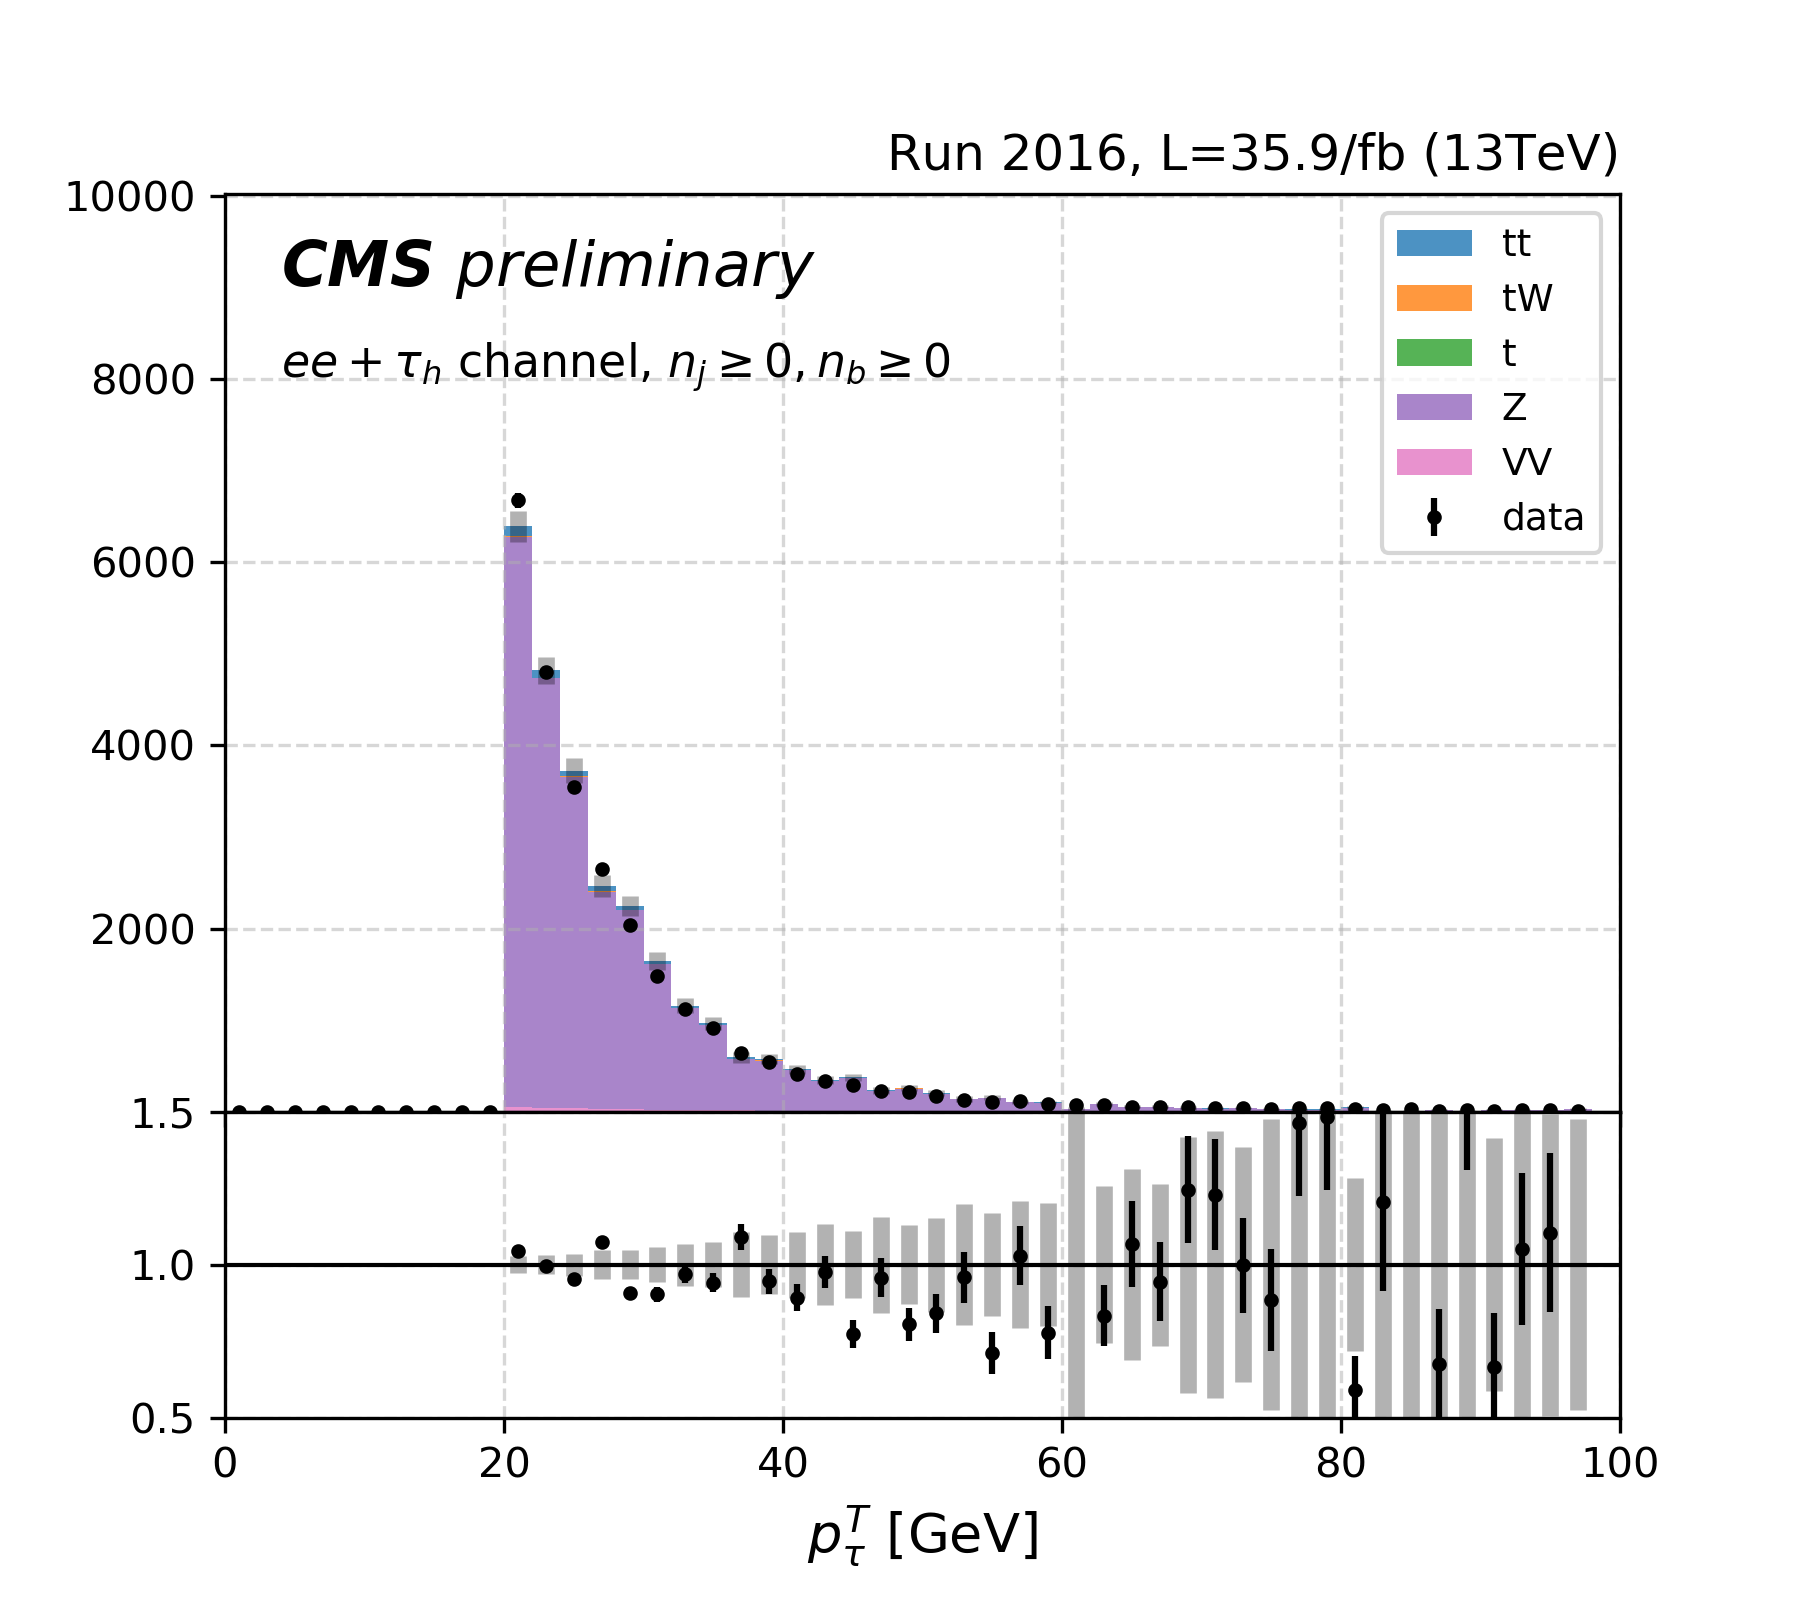
\includegraphics[width=0.4\textwidth]{chapters/Appendix/sectionJetToTauh/figures/eetau_tauPt_pickles_lltauTight.png}
    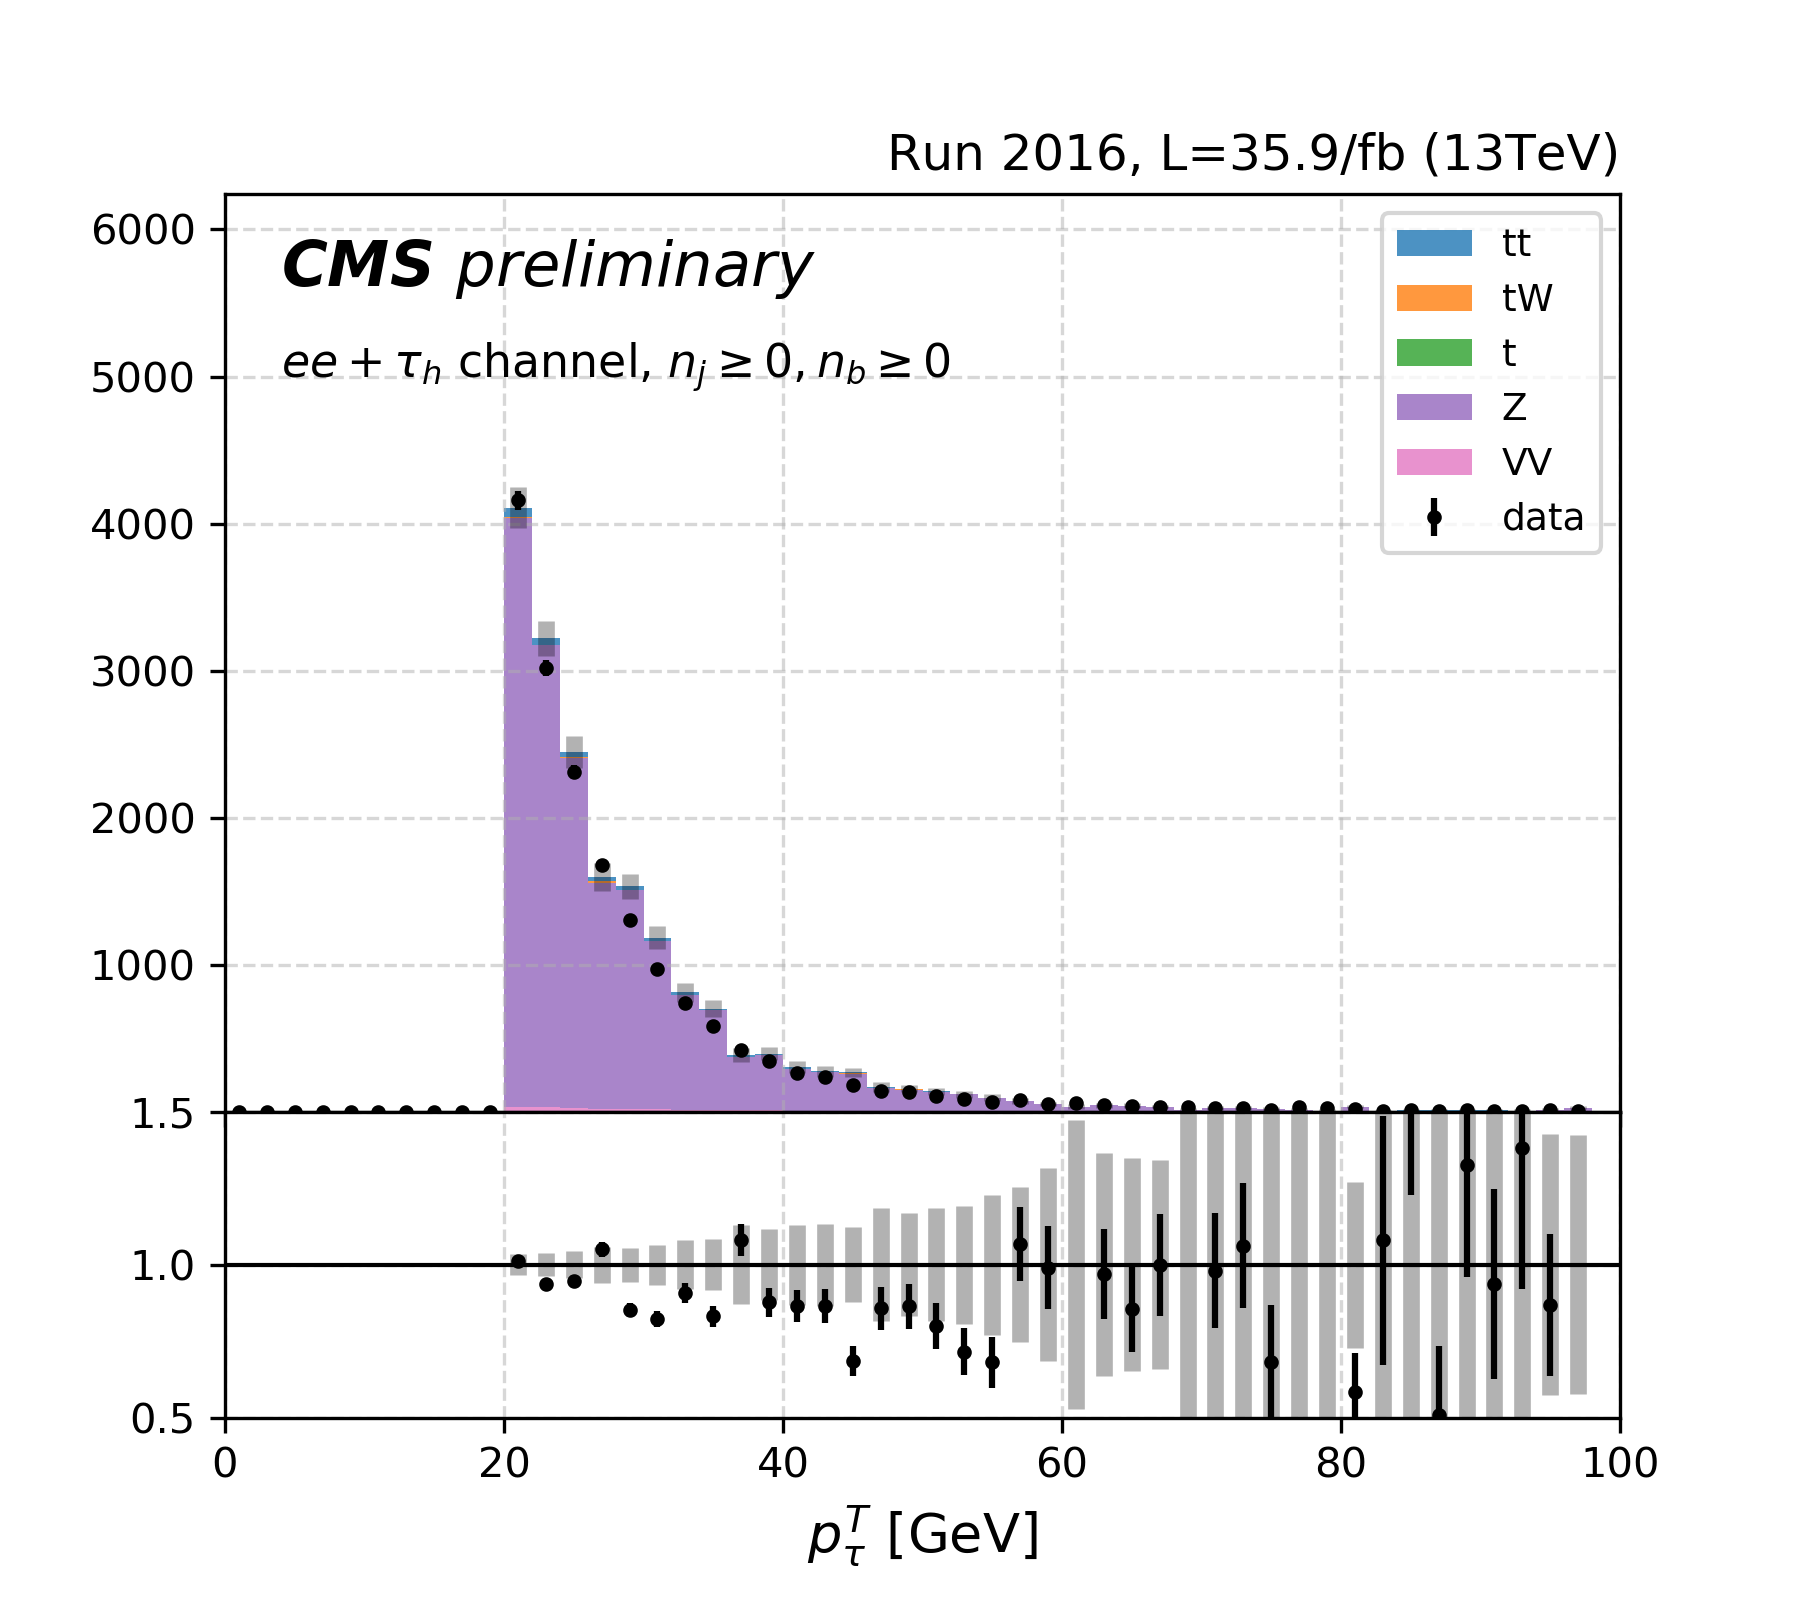
\includegraphics[width=0.4\textwidth]{chapters/Appendix/sectionJetToTauh/figures/eetau_tauPt_pickles_lltauVTight.png}
    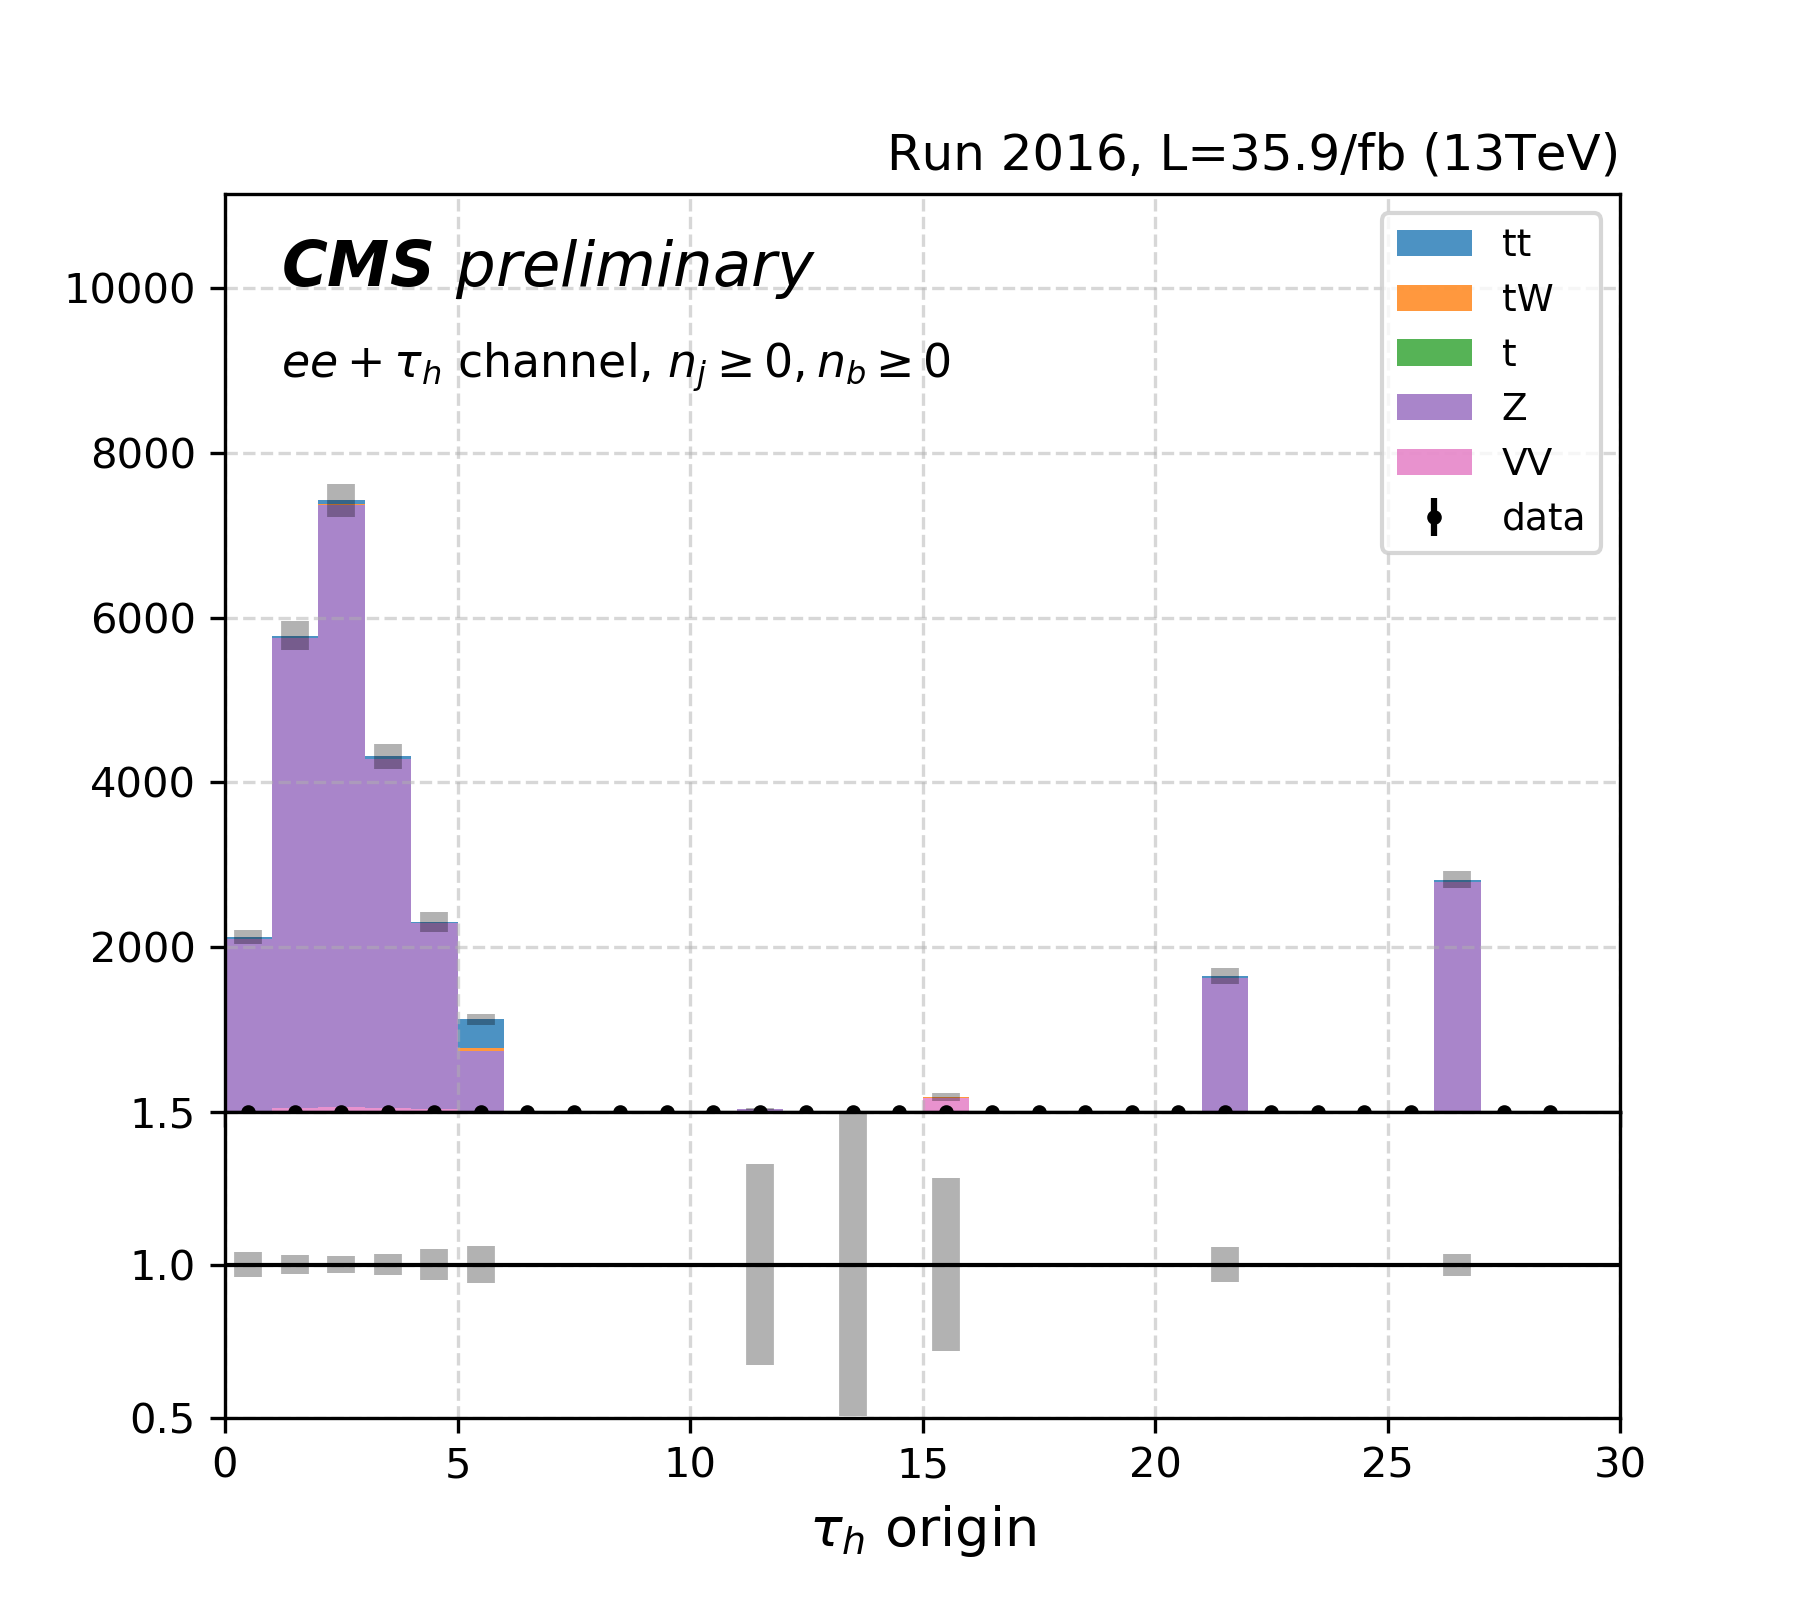
\includegraphics[width=0.4\textwidth]{chapters/Appendix/sectionJetToTauh/figures/eetau_tauGenFlavor_pickles_lltauTight.png}
    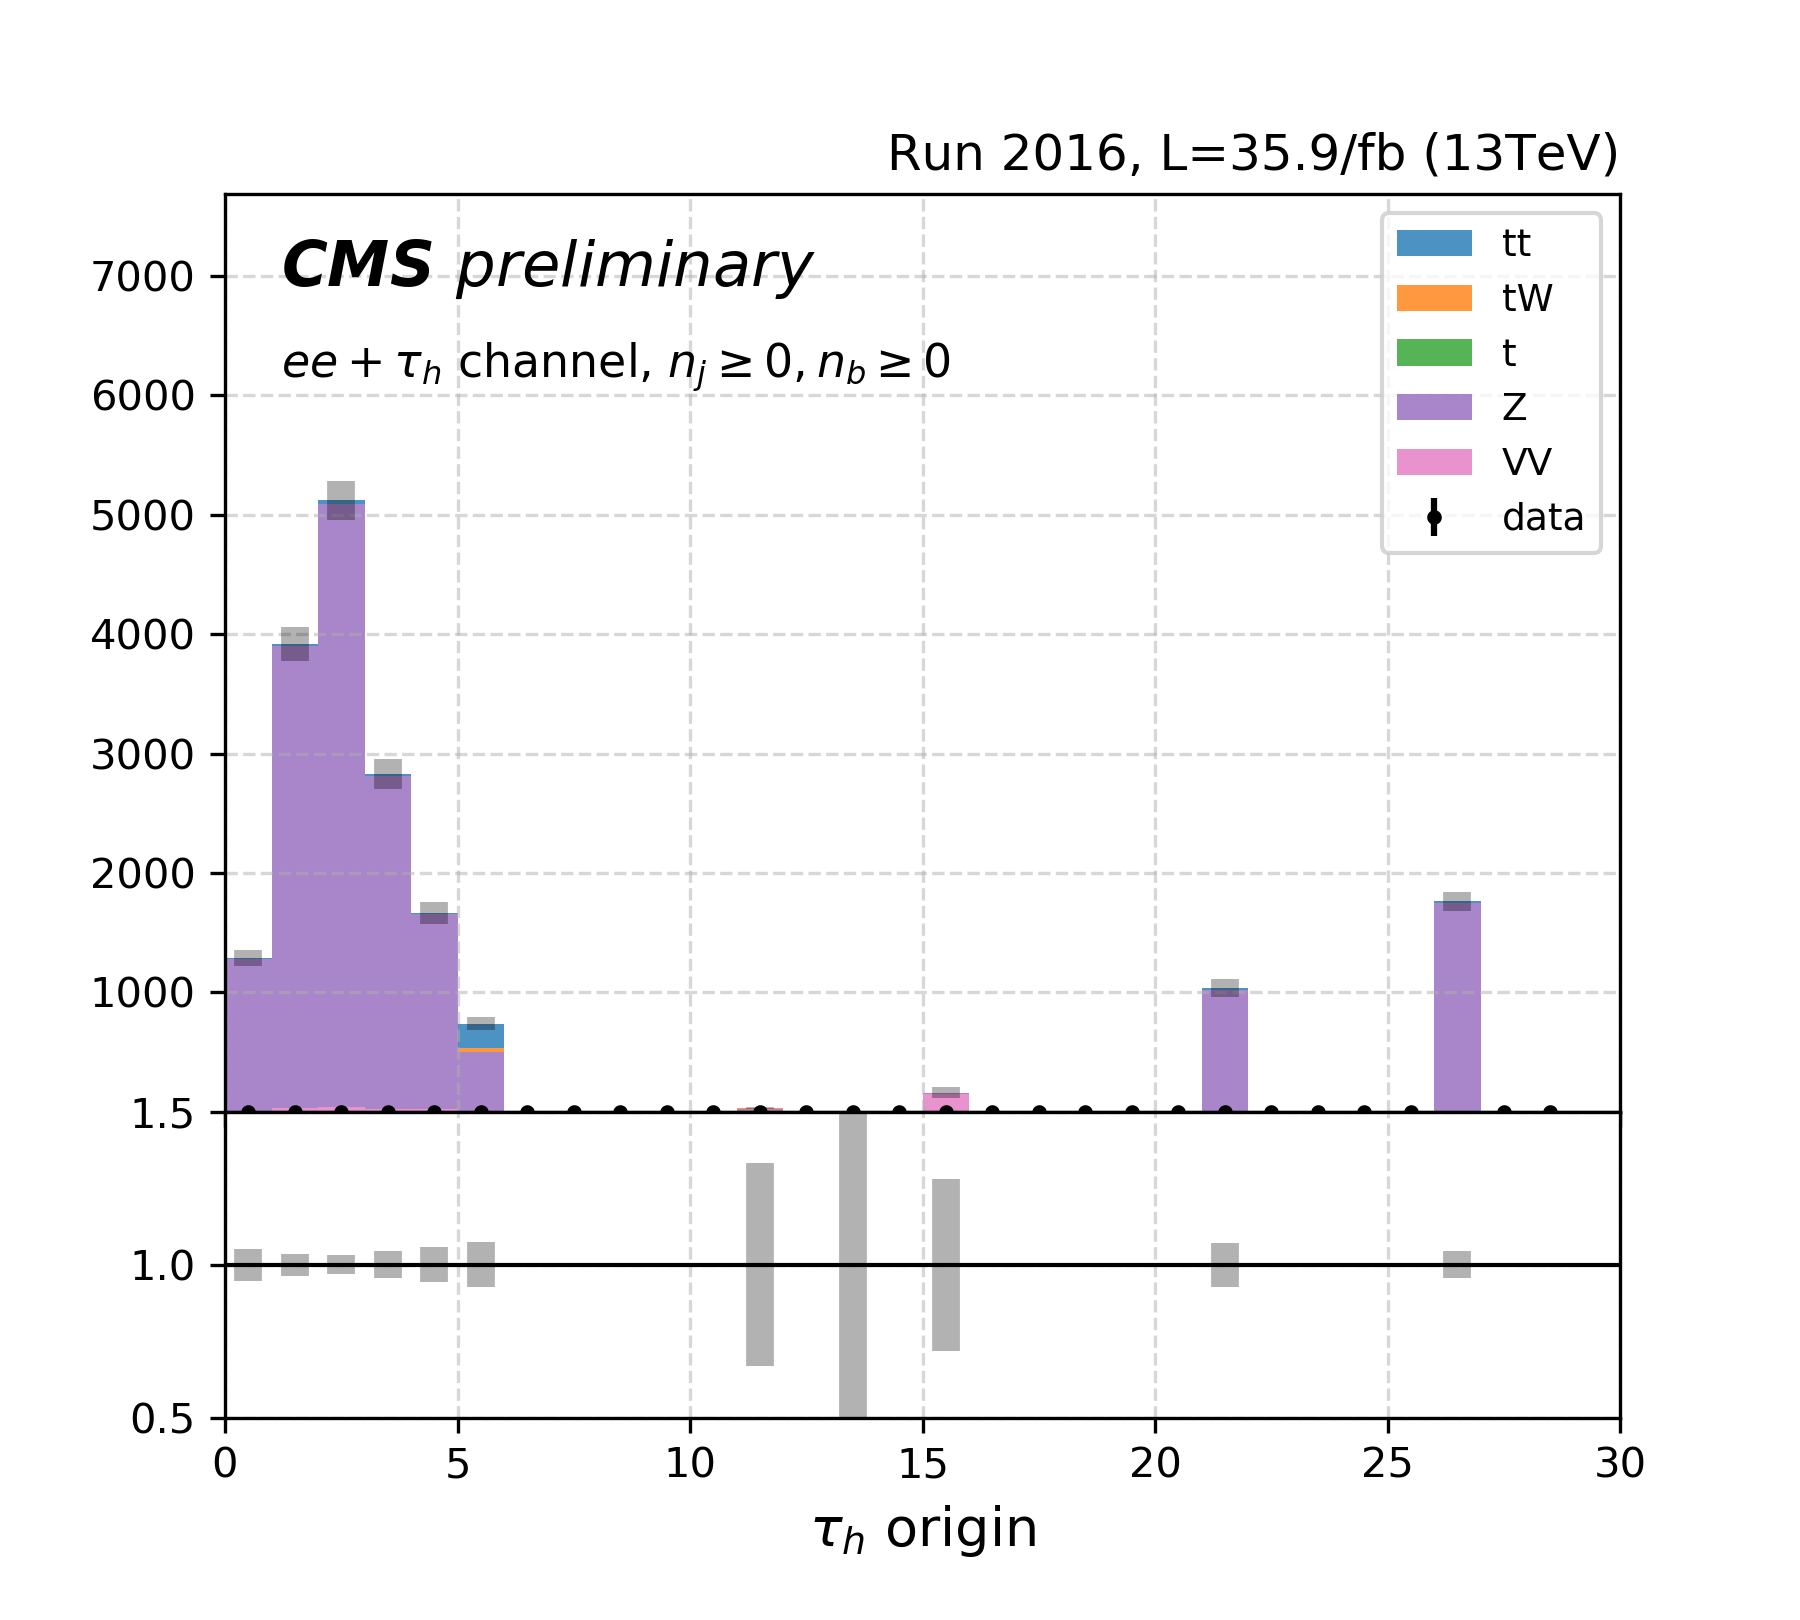
\includegraphics[width=0.4\textwidth]{chapters/Appendix/sectionJetToTauh/figures/eetau_tauGenFlavor_pickles_lltauVTight.png}
    \caption{Distributions of $m_{ee}$, $\tau pT$ and gen-level $\tau_h$ origin in the $ee+\tau$ channel. The left and right column shows the Tight and VTight $\tau_h$ WP respectively.}
    \label{fig:appendix:fakeTauId:eetau}
\end{figure}


The \pt spectrum of $\tau_h$ in $\mu\mu+\tau_h$, $ee+\tau_h$ and
$e\mu+\tau_h$ final states are shown in figure~\ref{fig:misidprefit}.
Because jet modeling of Z+jet is off in $n_j=0$ but good $n_j \geq 1$,
the events are split into $n_j=0$ and $n_j \geq 1$ to deal with jet
modeling in the Z+jet simulation. Both Tight and VTight working
points for $\tau_h$ isolation are included.

\begin{figure}
    \centering
    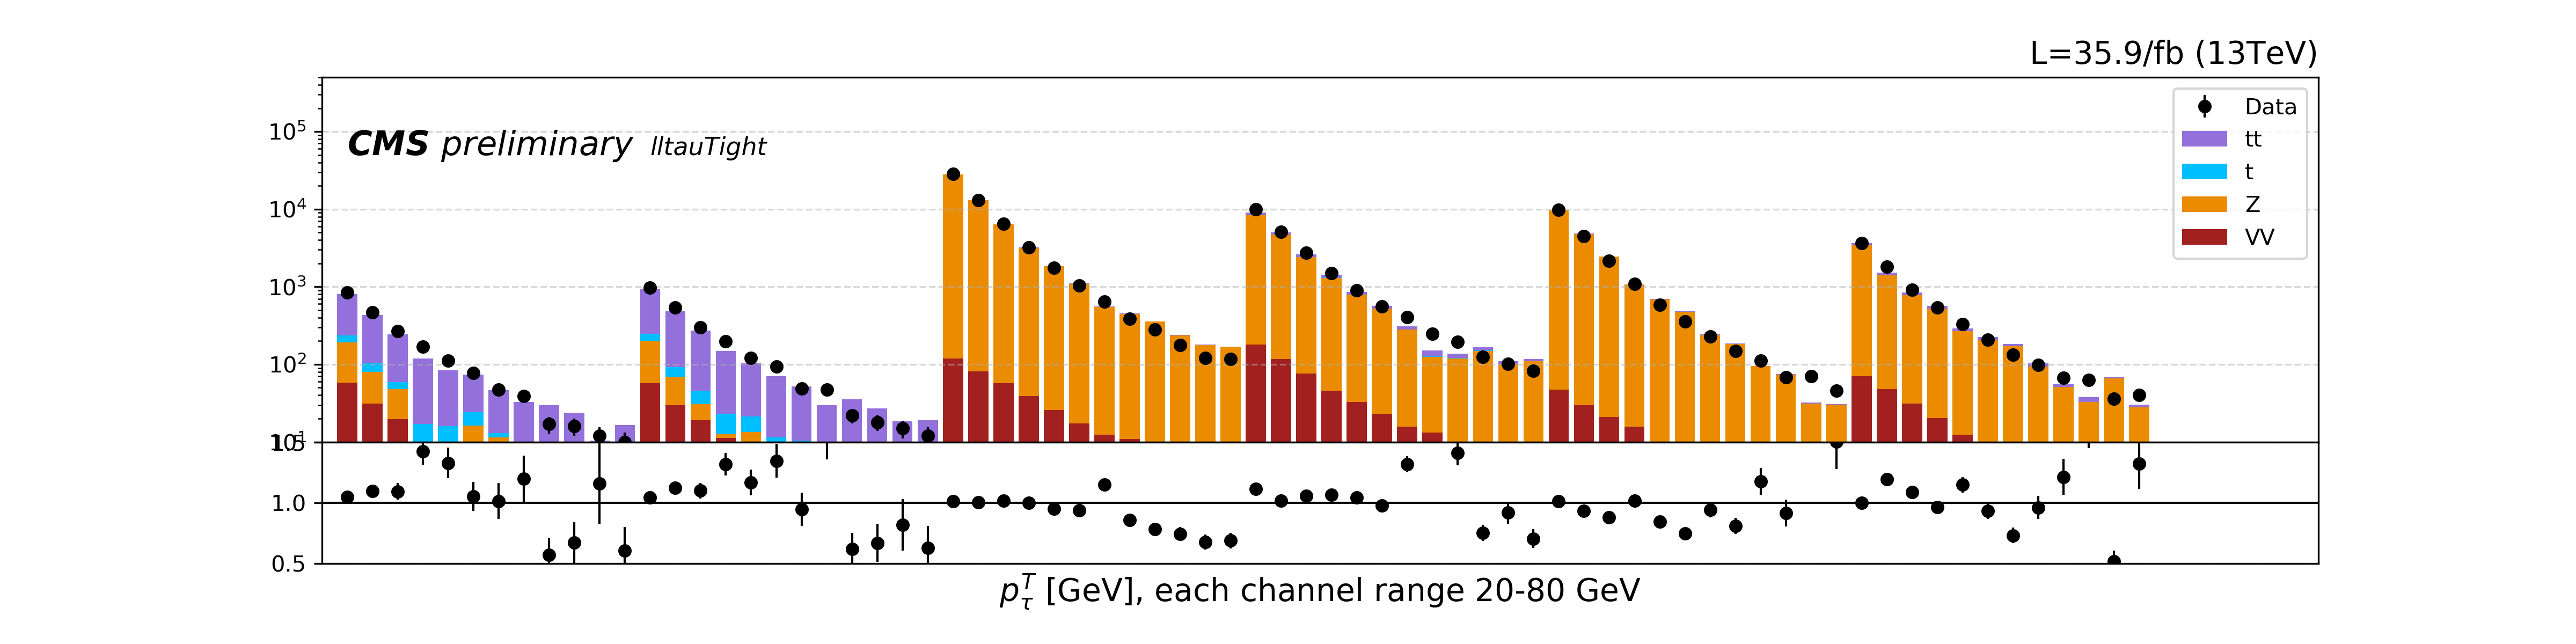
\includegraphics[width=0.99\textwidth]{chapters/Appendix/sectionJetToTauh/figures/2020_tauID_prefit_lltauTight.png}
    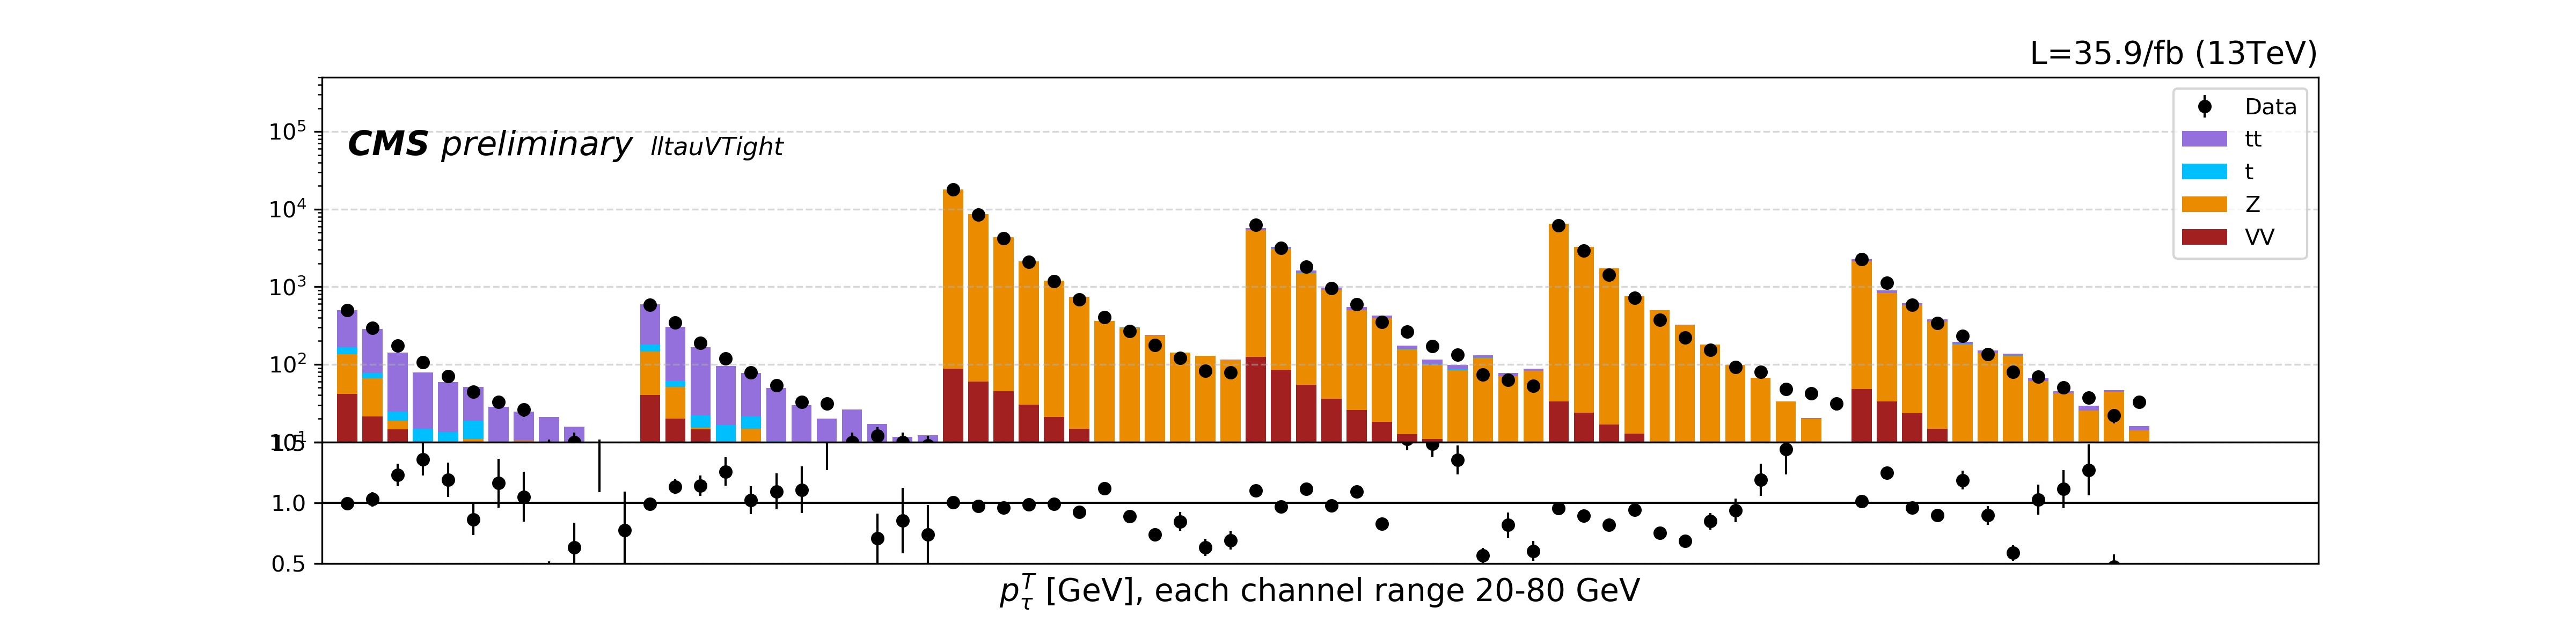
\includegraphics[width=0.99\textwidth]{chapters/Appendix/sectionJetToTauh/figures/2020_tauID_prefit_lltauVTight.png}
    \caption{Prefit distributions}
    \label{fig:appendix:fakeTauId:prefit}
\end{figure}

\begin{figure}
    \centering
    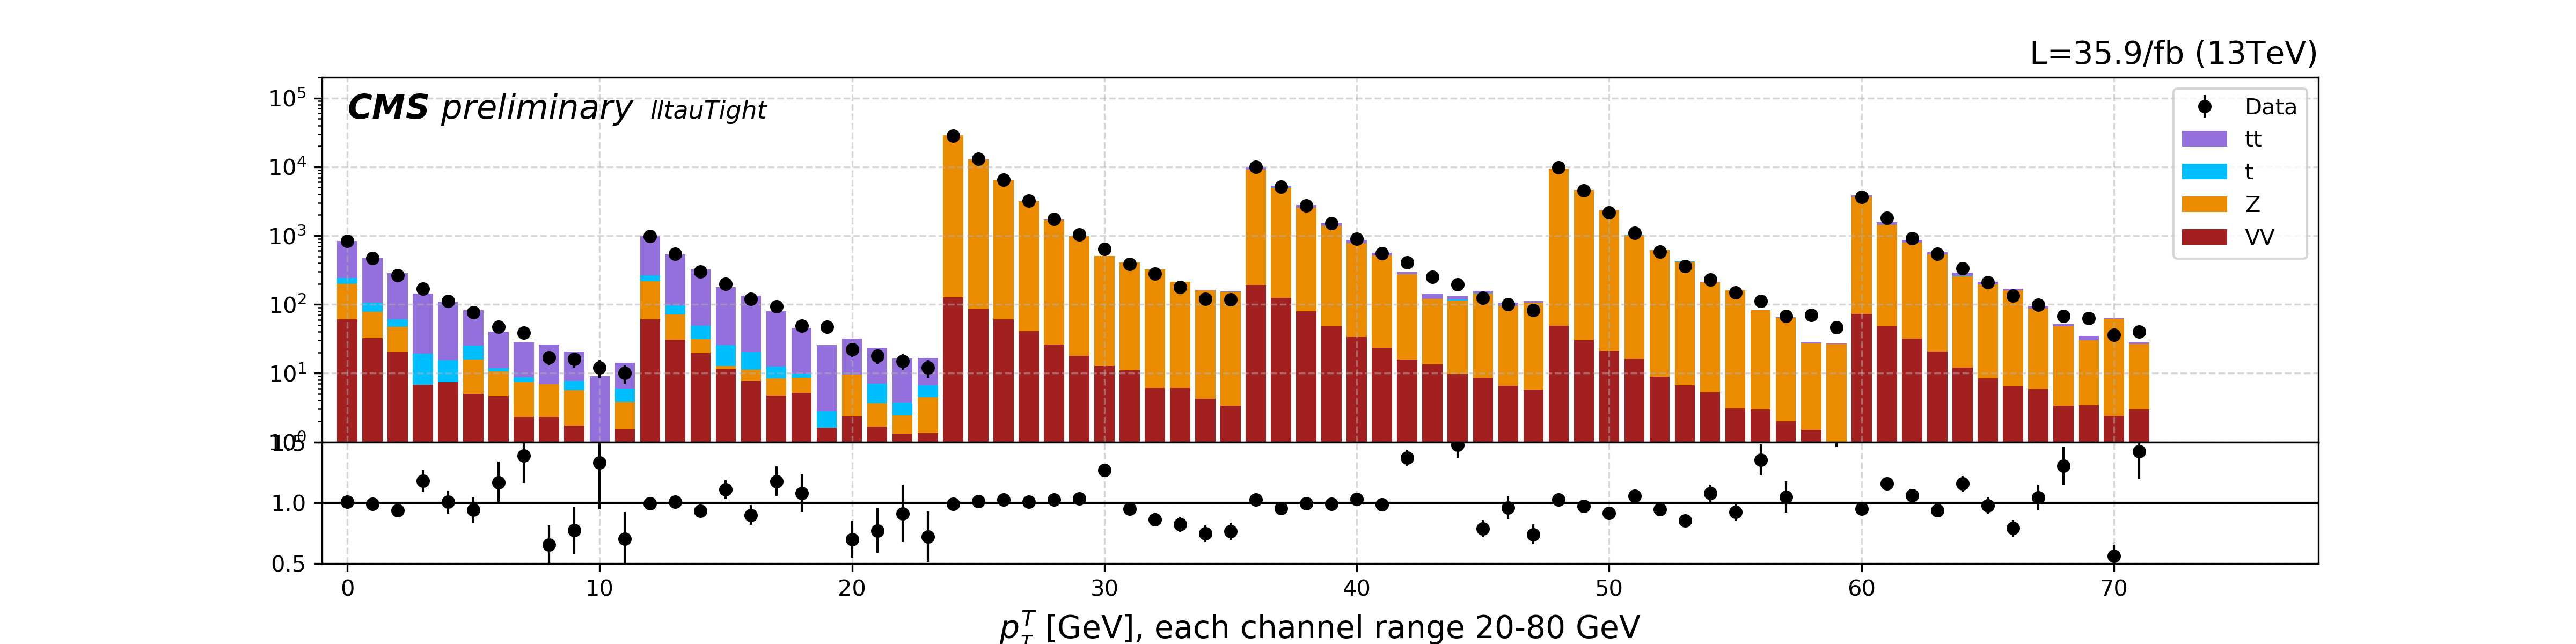
\includegraphics[width=0.99\textwidth]{chapters/Appendix/sectionJetToTauh/figures/2020_tauID_postfit_lltauTight.png}
    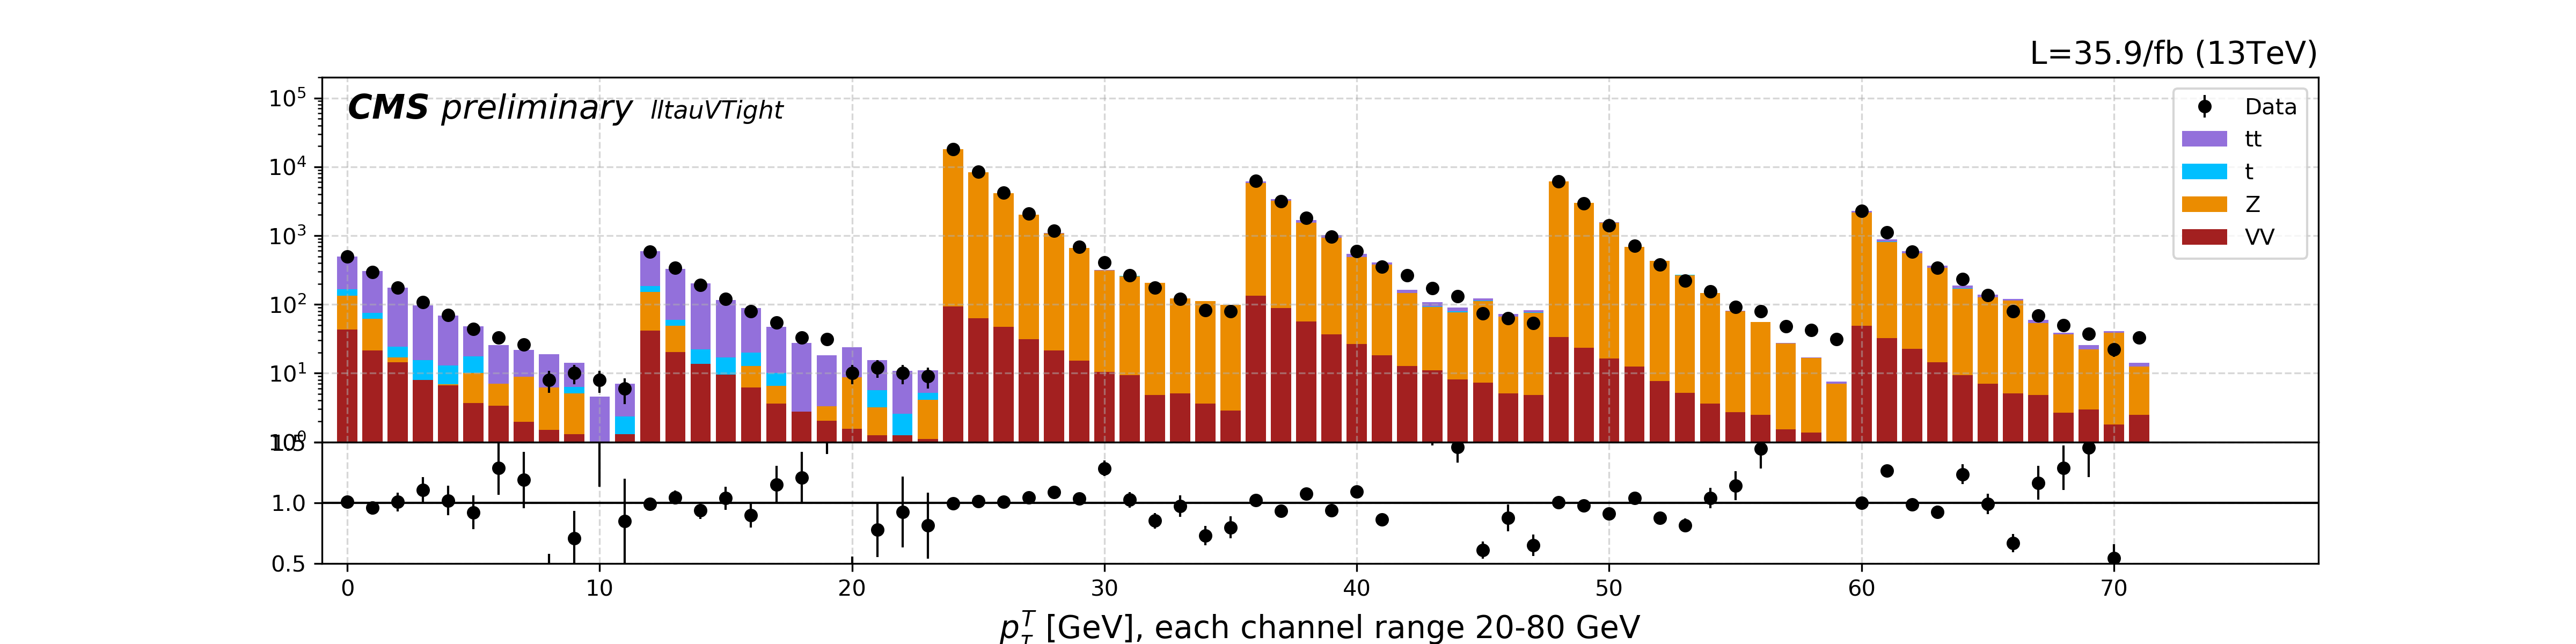
\includegraphics[width=0.99\textwidth]{chapters/Appendix/sectionJetToTauh/figures/2020_tauID_postfit_lltauVTight.png}
    \caption{Post distributions}
    \label{fig:appendix:fakeTauId:postfit}
\end{figure}

Then origin of selected $\tau_h$ are tagged based on MC truth.  For each
selected $\tau_h$, if there is a gen-level $\tau_h$ found within $\delta
R = 0.3$, the $\tau_h$ is tagged as true identification.  If not a true
identification, we try to match it with jet in the vetoed-jet collection
and tag it as $j \to \tau_h$, flavor of which equals to the MC flavor of
its jet correspondence.  In the rare case where multiple jet
correspondences are found, the one with highest pT is considered.  If
neither gen-level $\tau_h$ match nor jet correspondence are found, the
$\tau_h$ is untagged, which mainly due to $e \to \tau_h$. The gen-level 
origin of $\tau_h$ are included in Figure~\label{fig:appendix:fakeTauId:emutau},
\label{fig:appendix:fakeTauId:mumutau},\label{fig:appendix:fakeTauId:eetau}.


To measure $SF (j \to \tau_h)$, we breakdown simulated events by 5
processes and 6 $\tau_h$ flavors and performed a template fit.  The free
parameters are $SF (j \to \tau_h)$ in 6 pT bins from 20-80 GeV. To
understand the dependency of SF on jet flavor, we also looked at the fit
scenario where $SF (j \to \tau_h)$ are split into $SF (b \to \tau_h)$
and $SF (q \to \tau_h)$ as free parameters.  The systematical
uncertainty, including cross sections, luminosity, electron/muon
efficiency, are taken into account as nuisance parameters in the fit.
The result of $SF (j\to \tau_h)$ is shown in figure~\ref{fig:appendix:fakeTauId:fit}. 



In shape analysis, the
uncertainty of $SF (j \to \tau_h)$ will be used as prefit uncertainty of
the corresponding nuisance parameters.  In counting analysis, $SF (j \to
\tau_h)$ will be variate according to its uncertainty, leading to the
change of efficiency matrix and final results.




\begin{figure}
    \centering
    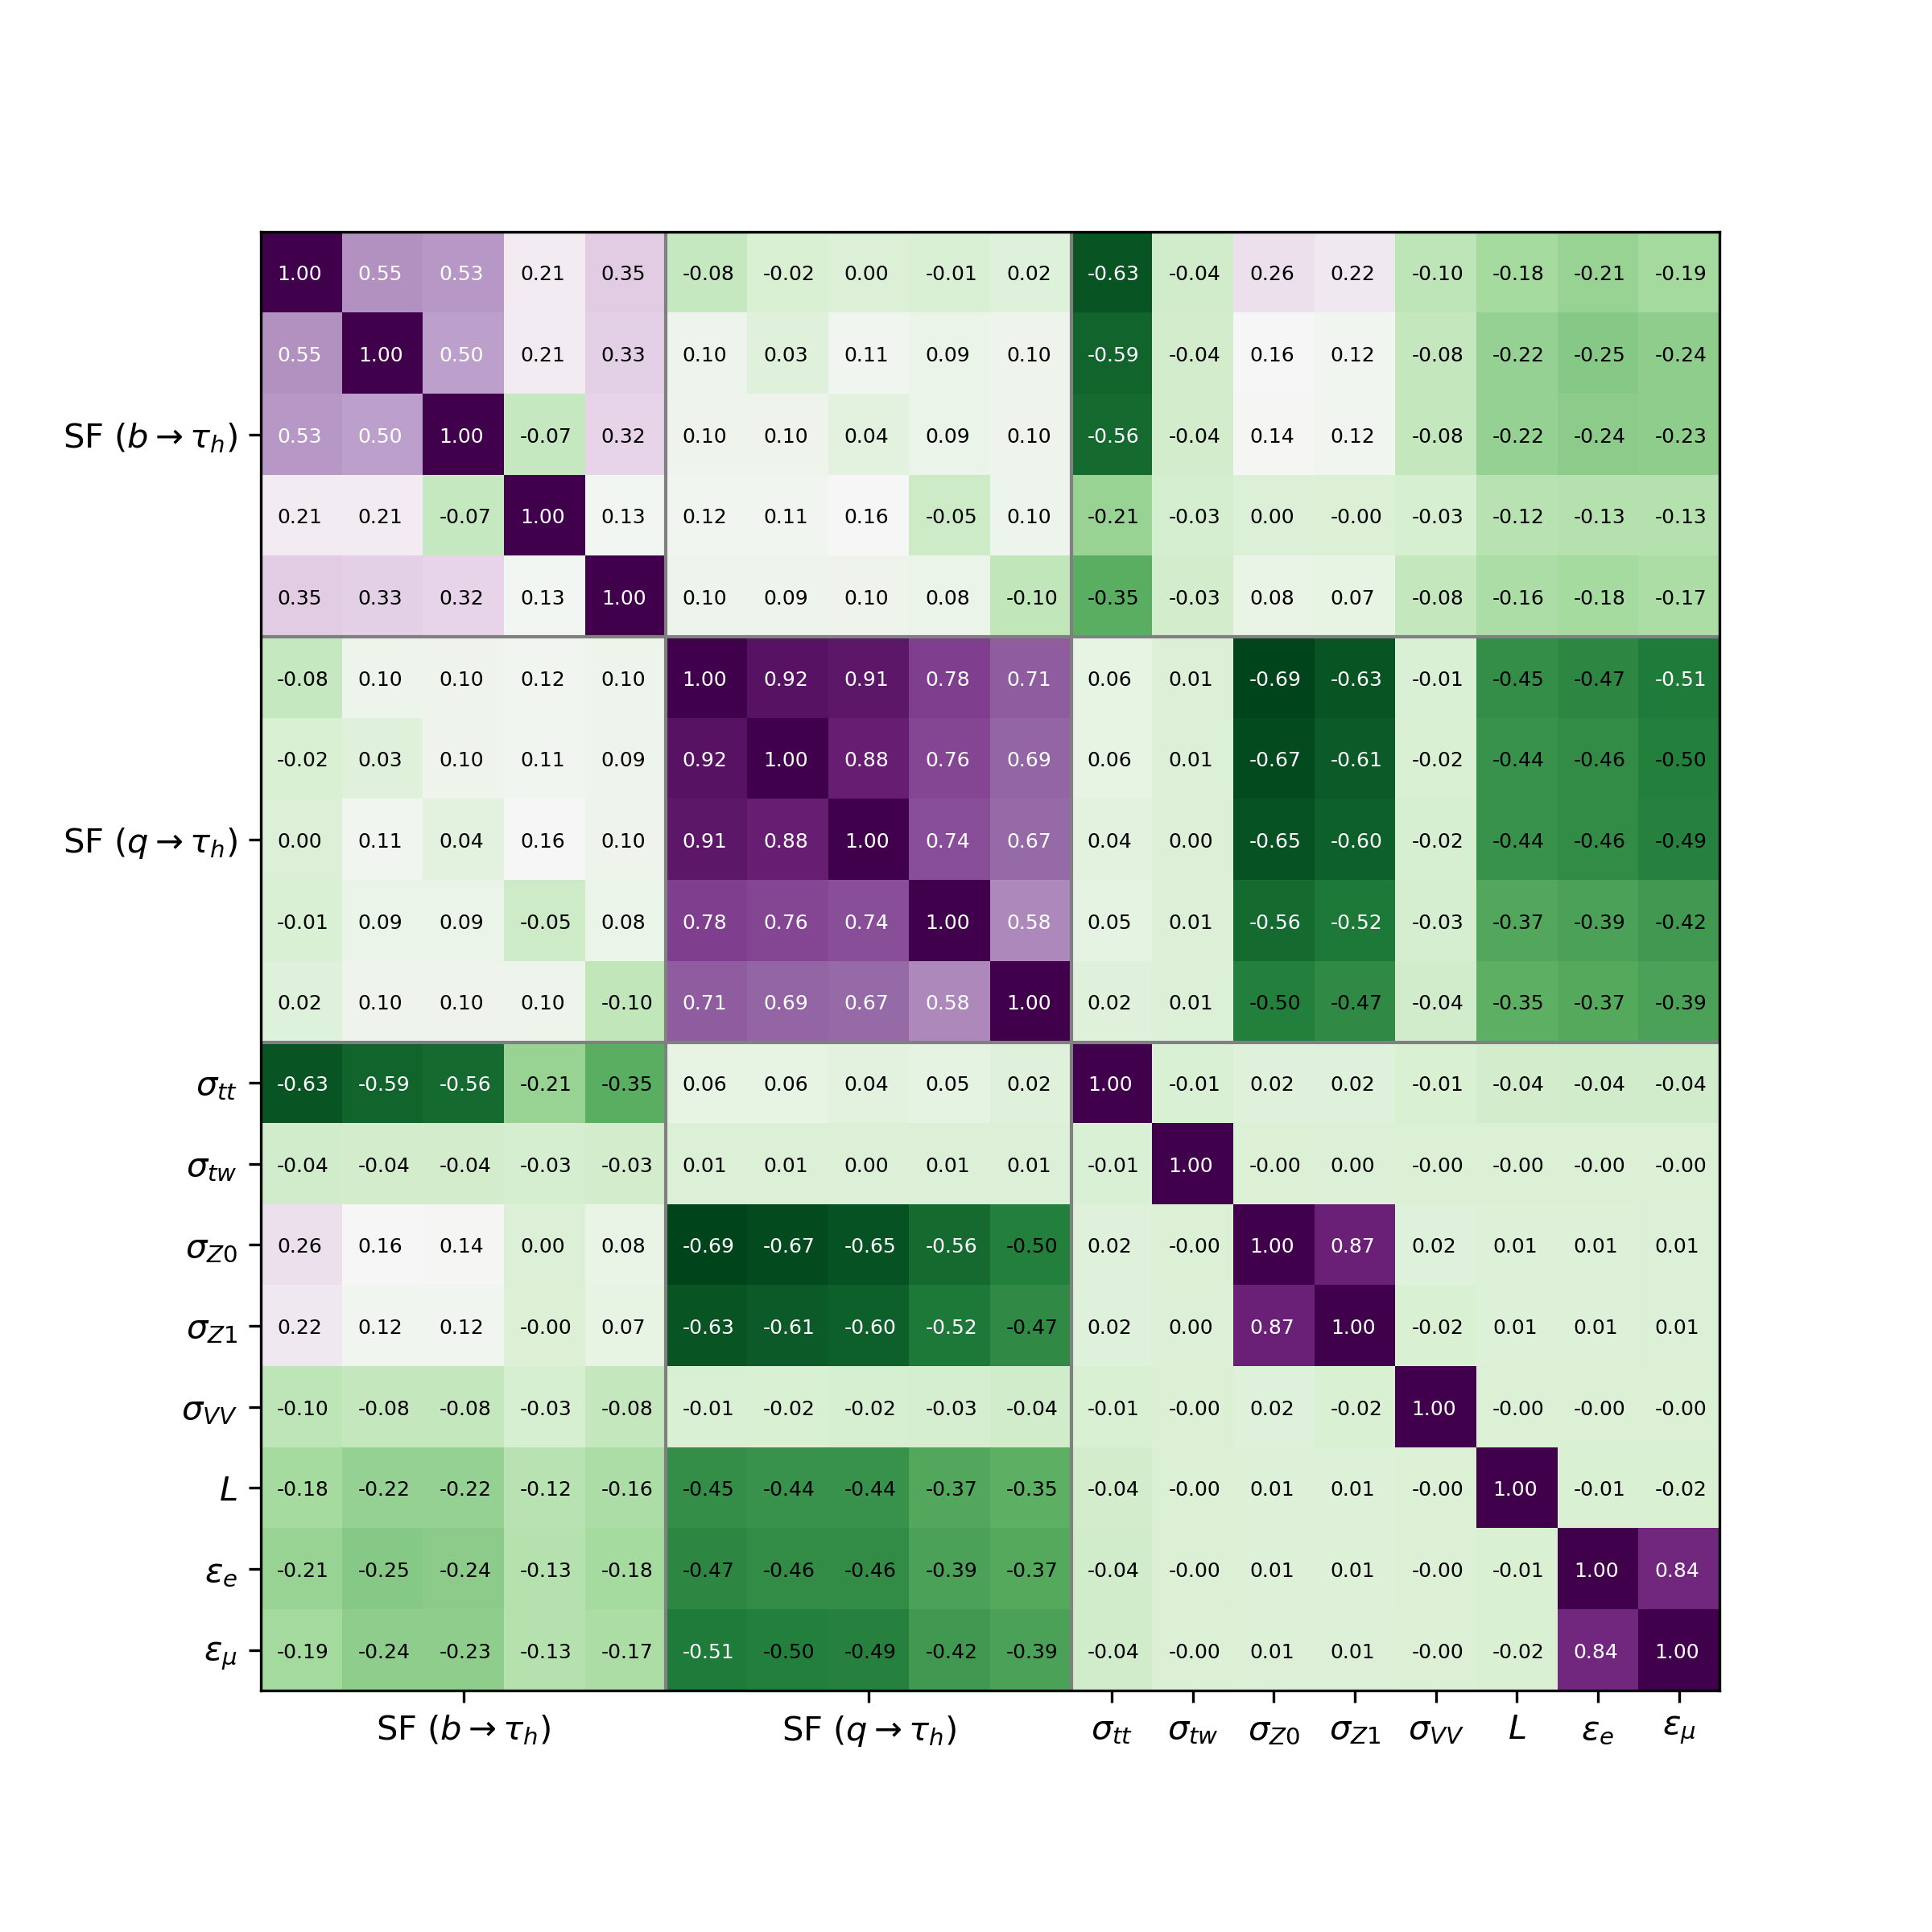
\includegraphics[width=0.49\textwidth]{chapters/Appendix/sectionJetToTauh/figures/corr2_lltauTight_splitJetFlavor.png}
    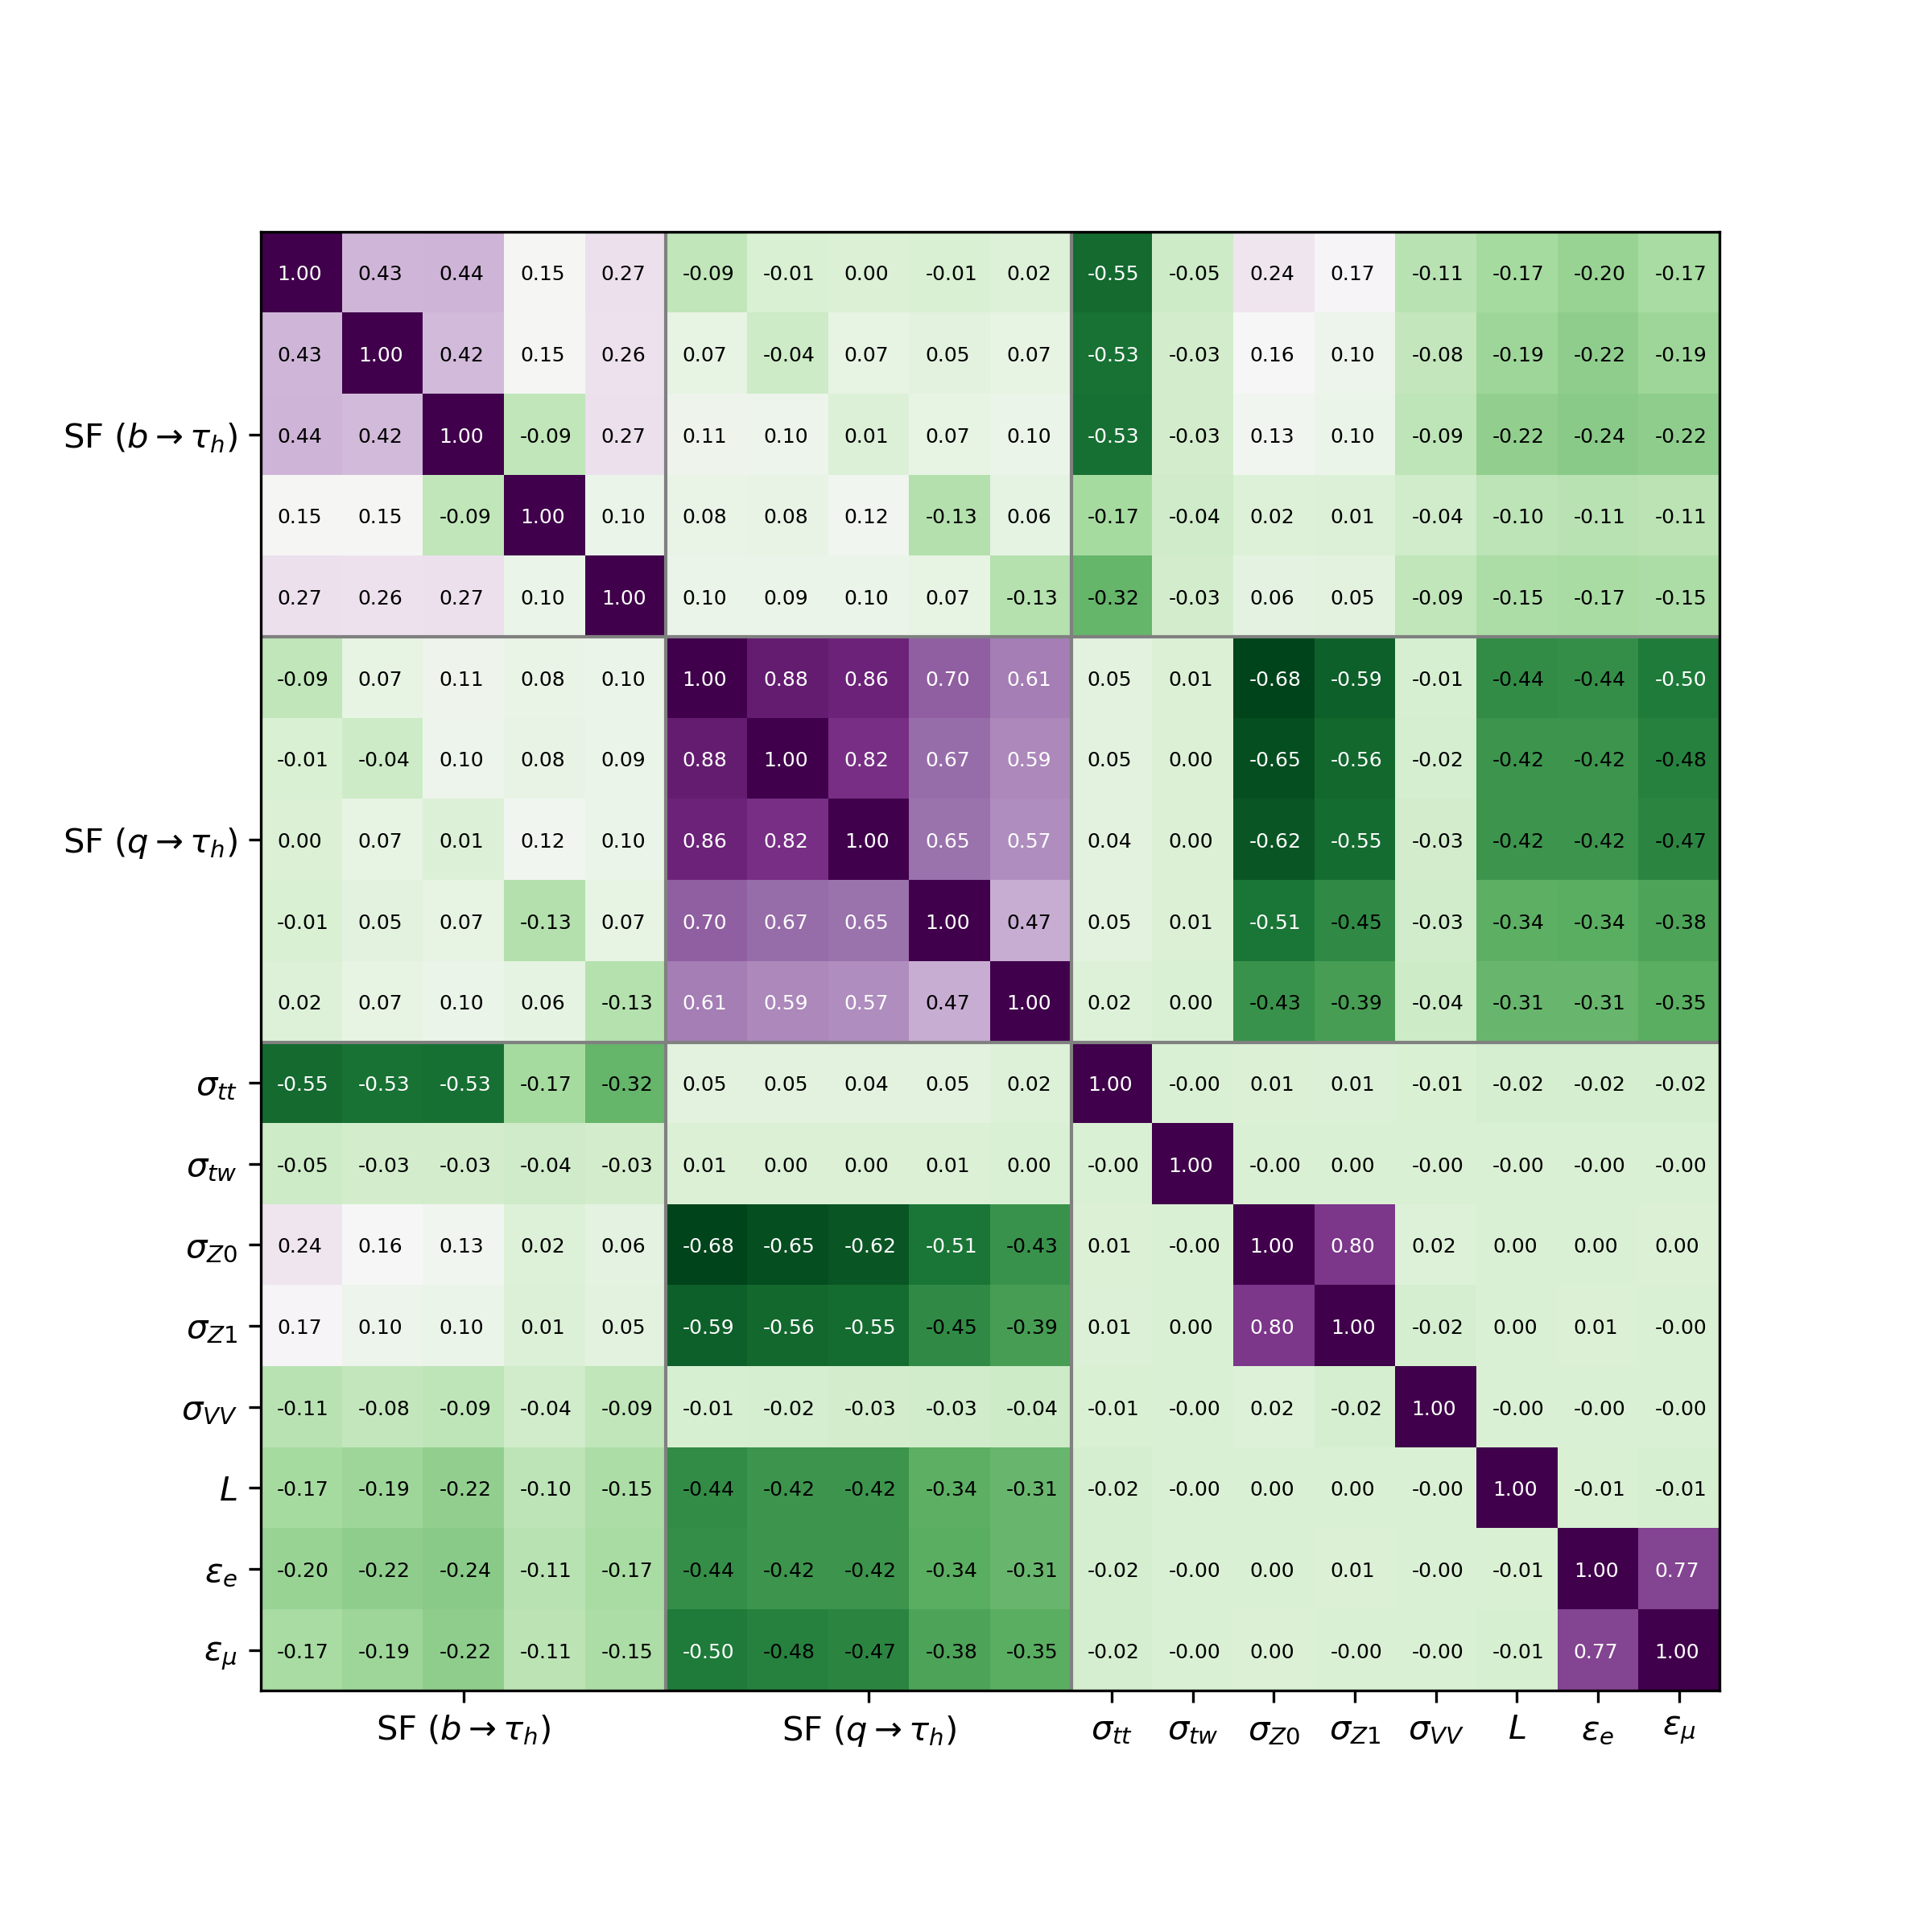
\includegraphics[width=0.49\textwidth]{chapters/Appendix/sectionJetToTauh/figures/corr2_lltauVTight_splitJetFlavor.png}
    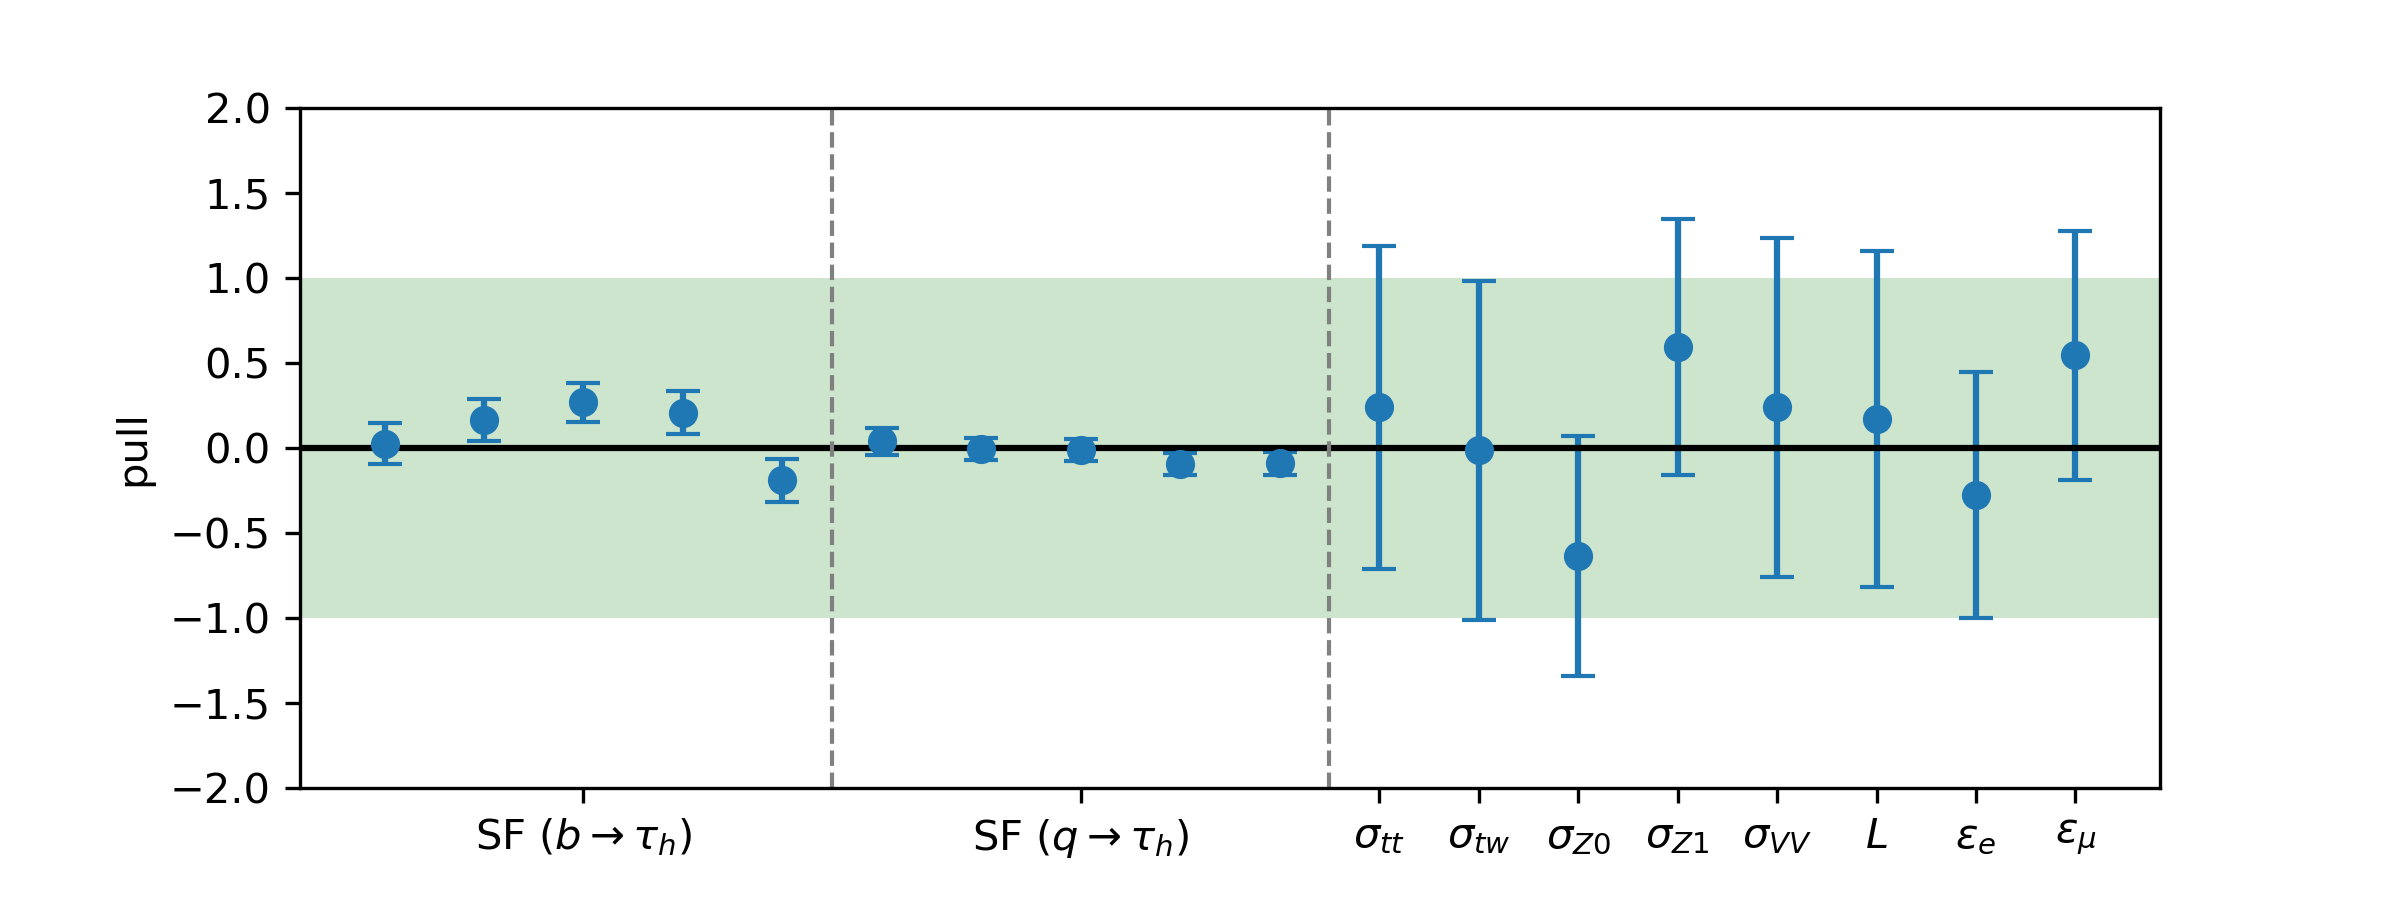
\includegraphics[width=0.49\textwidth]{chapters/Appendix/sectionJetToTauh/figures/pull2_lltauTight_splitJetFlavor.png}
    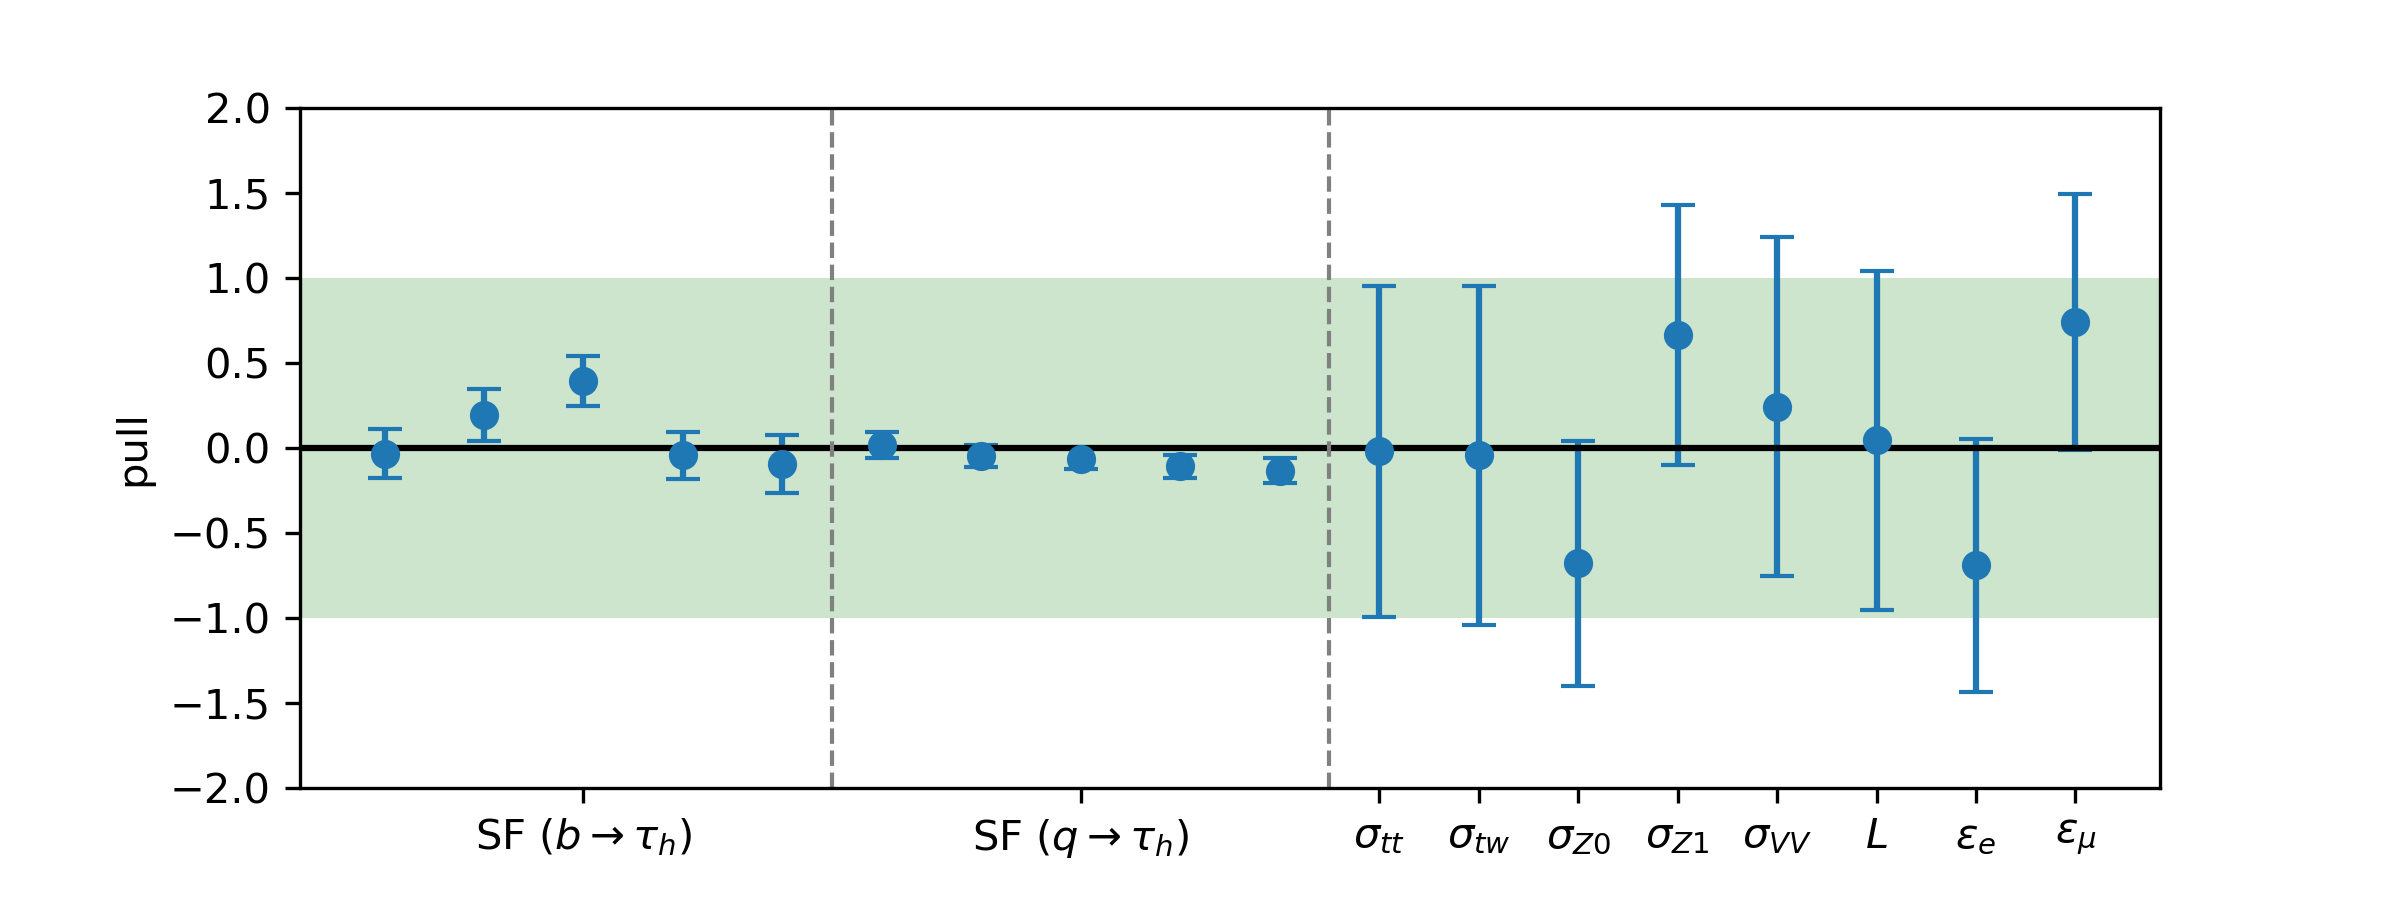
\includegraphics[width=0.49\textwidth]{chapters/Appendix/sectionJetToTauh/figures/pull2_lltauVTight_splitJetFlavor.png}
    \caption{The correlation coefficients and pull of fitting parameters}
    \label{fig:appendix:fakeTauId:fitparam}
\end{figure}

\begin{figure}
    \centering
    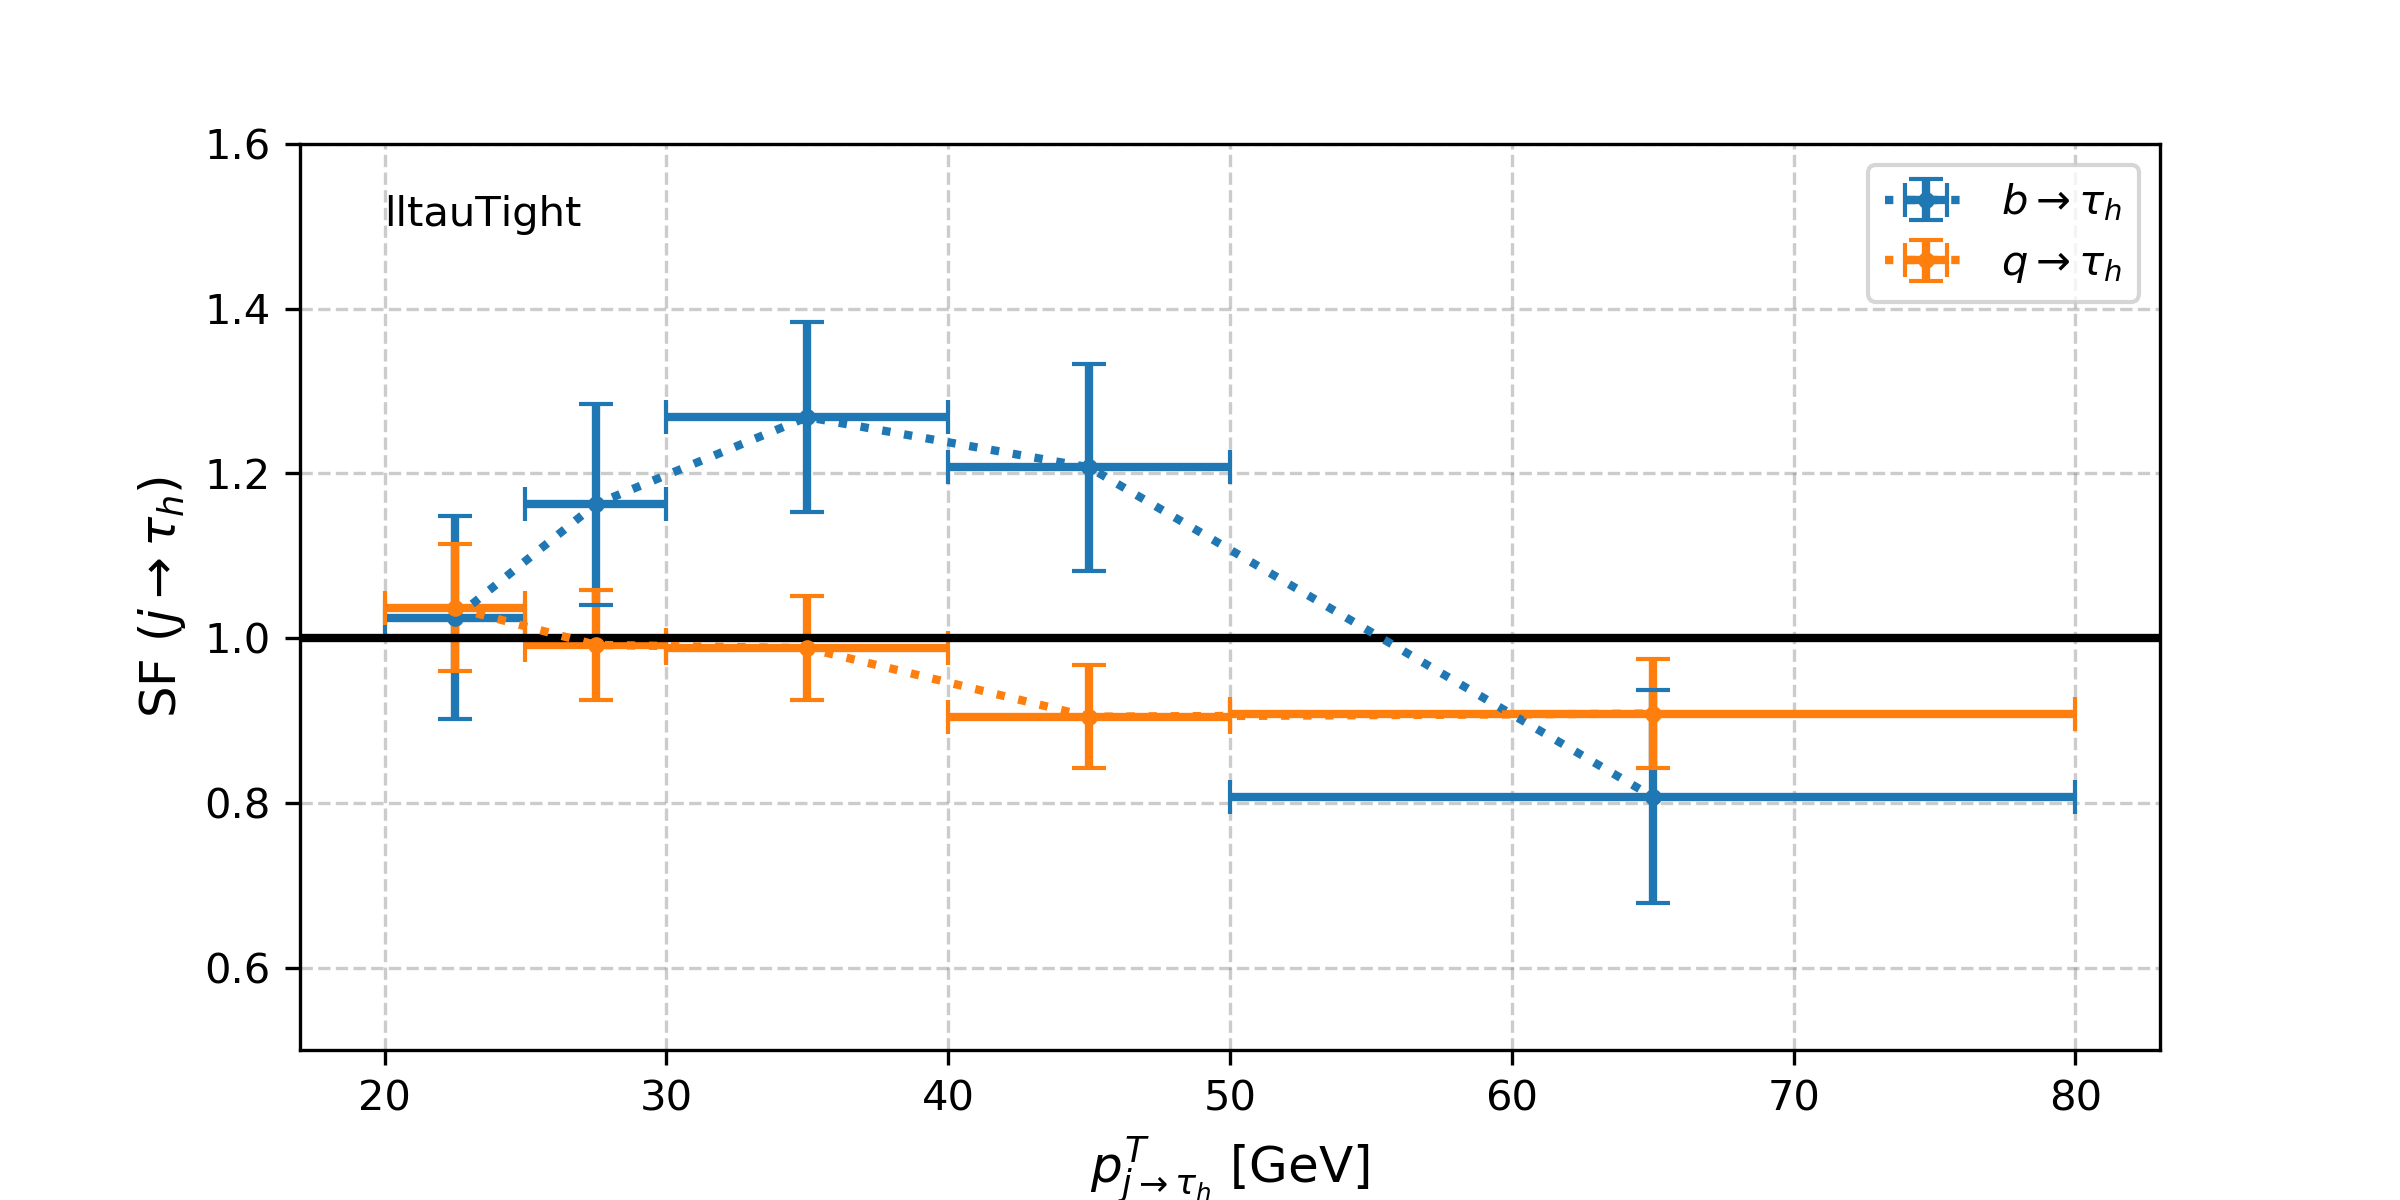
\includegraphics[width=0.49\textwidth]{chapters/Appendix/sectionJetToTauh/figures/fit2_ptflavor2_lltauTight.png}
    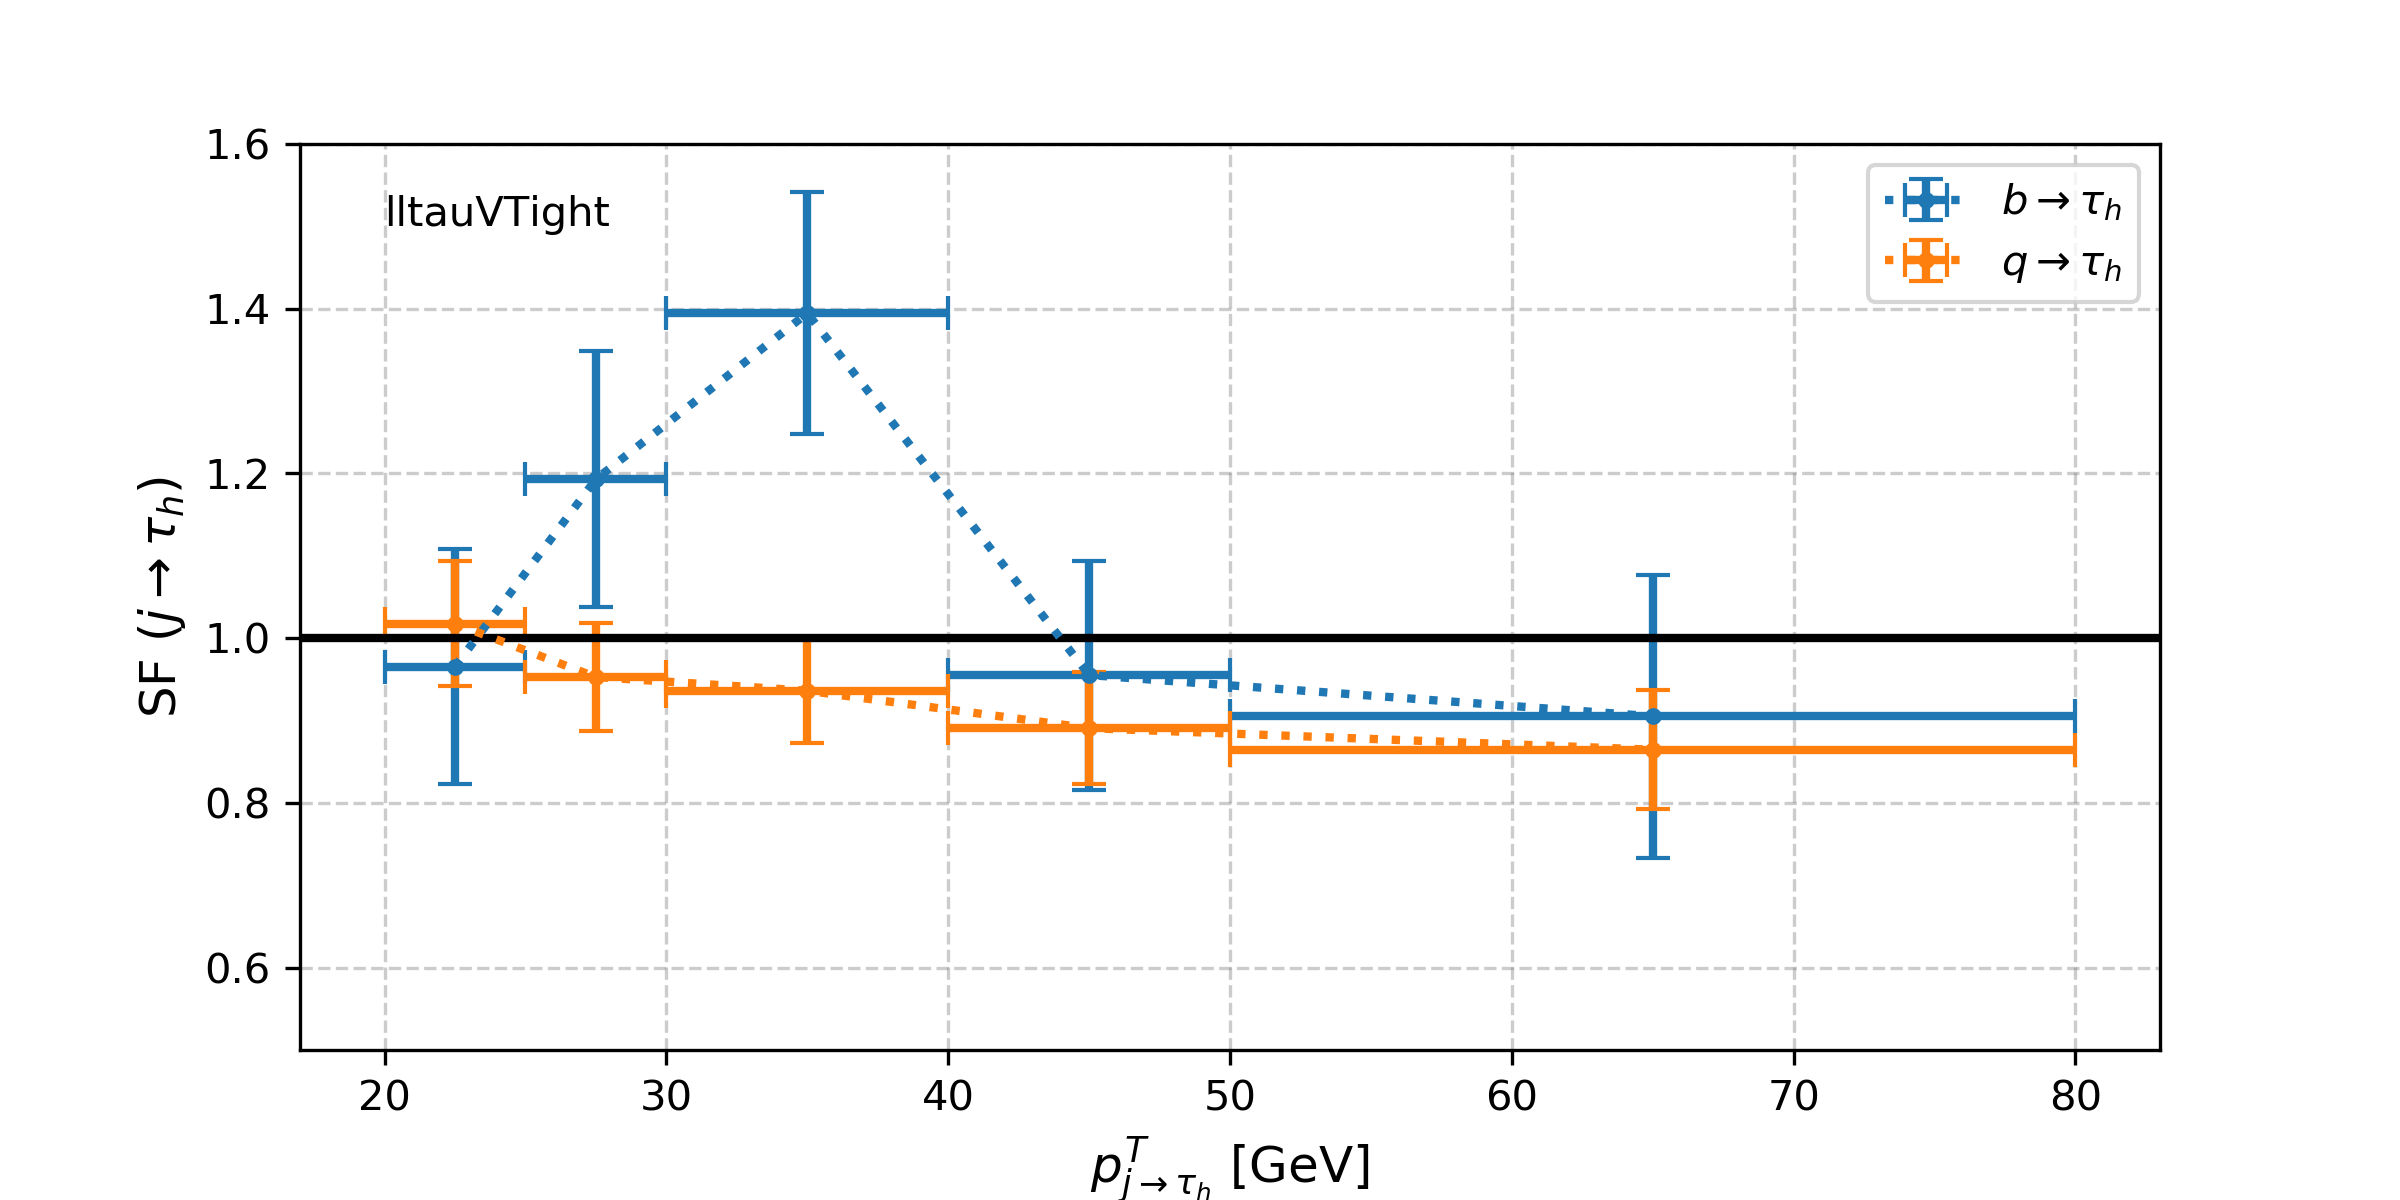
\includegraphics[width=0.49\textwidth]{chapters/Appendix/sectionJetToTauh/figures/fit2_ptflavor2_lltauVTight.png}
    \caption{SF}
    \label{fig:appendix:fakeTauId:fit}
\end{figure}

\begin{table}[h]
    \setlength{\tabcolsep}{6pt} % Default value: 6pt
    \renewcommand{\arraystretch}{1.5} % Default value: 1
    \begin{tabular}{c|ccccc}
    \hline
    $p^T_{\tau_h}$ [GeV]  & 20-25         & 25-30         & 30-40         & 40-50         & 50-80         \\
    \hline
    $SF(b\to Tight \cdot \tau_h)$  & $1.02\pm0.12$ & $1.16\pm0.12$ & $1.27\pm0.11$ & $1.21\pm0.13$ & $0.81\pm0.13$ \\
    $SF(q\to Tight \cdot \tau_h)$  & $1.04\pm0.08$ & $0.99\pm0.07$ & $0.99\pm0.06$ & $0.90\pm0.06$ & $0.91\pm0.07$ \\
    \hline
    $SF(b\to VTight \cdot\tau_h)$ & $0.97\pm0.14$ & $1.19\pm0.16$ & $1.39\pm0.15$ & $0.96\pm0.14$ & $0.91\pm0.17$ \\
    $SF(q\to VTight \cdot\tau_h)$ & $1.02\pm0.08$ & $0.95\pm0.07$ & $0.94\pm0.06$ & $0.89\pm0.07$ & $0.86\pm0.07$ \\
    \hline
    \end{tabular}
    \caption{ $SF (j\to \tau_h)$ for Tight and VTight tau MVA}
\end{table}

\FloatBarrier